\chapter{A complete methodology for the implementation of XFEM inclusive models}
\label{sec:a_complete_methodology_for_the_implementation_of_XFEM_inclusive_models}

% -----------------------------------------------------------------------------
% Abstract.

This document was written in 2012 as an internal implementation manual for future developers of our code, the Finite Element Multi-Disciplinary Optimization Code (femdoc).

This report offers a background into the eXtended Finite Element Method as a tool to solve the shortcomings of the classical Finite Element Method. An example of such is the numerical solution to problems with different material topologies (i.e. discontinuities). The XFEM uses level set functions to track the location of these discontinuities. The report also provides algorithms for locating these discontinuities and subsequently dividing the domain into sub-domains capable of integration. This report ultimately expounds upon how to effectively apply the local enrichment functions that the XFEM standard approximation requires at the nodes where the discontinuities occur.

The reader may skip this section, as it focuses on the algorithmic implementation of the framework and most of its content is intended for software developers.

% -----------------------------------------------------------------------------
% Chapters.

% XFEM: Background.
\chapter{Introduction}
\label{sec:introduction}

The goal of this thesis proposal is to introduce a unified topology optimization framework that uses the \textbf{L}evel \textbf{S}et \textbf{M}ethod (LSM) to describe the design geometry and the e\textbf{X}tended \textbf{F}inite \textbf{E}lement \textbf{M}ethod (XFEM) to solve the governing equations and measure the performance of the design. The framework will be referred to as the LSM-XFEM optimization method.

Topology optimization approaches (see Sections \ref{sec:optimization} and \ref{sec:intro_topology_optimization}) seek the optimal geometry and/or material layout of a body within a given design domain. Popular schemes, such as density methods (Section \ref{sec:density_topology_approaches}), have been widely applied to topology optimization of different physics, such as structures, fluid dynamics, etc. In structural topology optimization, the density method works by transforming the structural optimization problem into a standard nonlinear program where the design variables are coefficients of the governing equation. These design variables are introduced as the material density of the finite elements. Density approaches cannot describe the physics at the phase interface accurately without extensive mesh refinement. This may lead to unphysical responses (Section \ref{sec:SIMP_discussion}). Therefore, problems that require an accurate description of the boundary conditions at the interface may not be suited for density approaches.  The use of level set methods in topology optimization emerged as an alternative to the density approach. Level set methods (Section \ref{sec:intro_level_set_method}) are able to provide an accurate representation of the layout by dividing the design domain into phase regions, where each region may represent a different physics or a different material, as shown in Figure \ref{fig:level_set_circle_description}.
%
\begin{figure}
	\centering
	\begin{tabularx}{\linewidth}{XX}
		\subfloat[]{
			\label{fig:level_set_circle_func_1}
			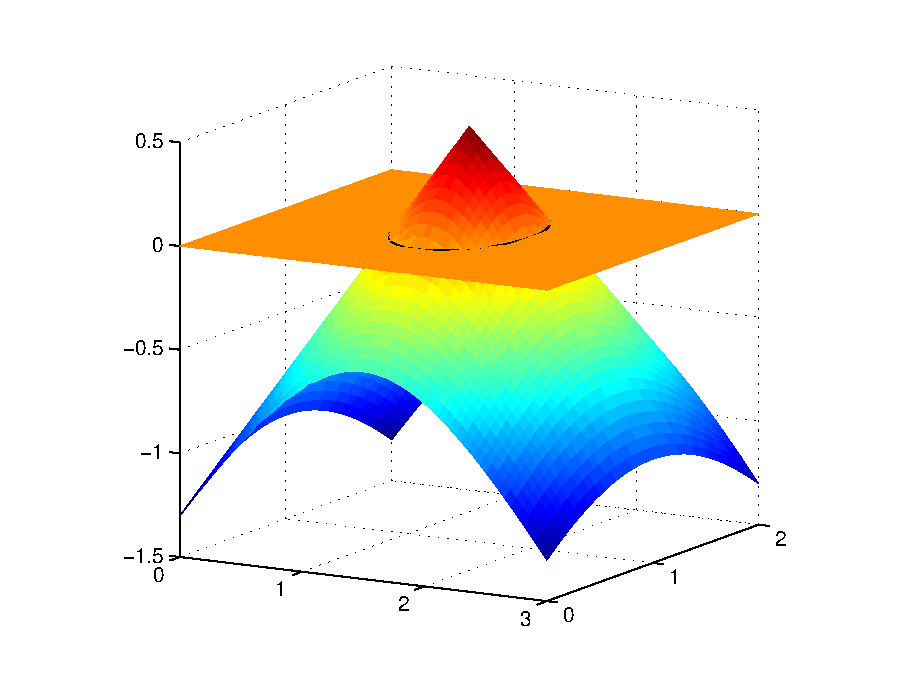
\includegraphics[width=\linewidth]{level_set_circle_func_050.eps}
		} &
		\subfloat[]{
			\label{fig:level_set_circle_domain_1}
			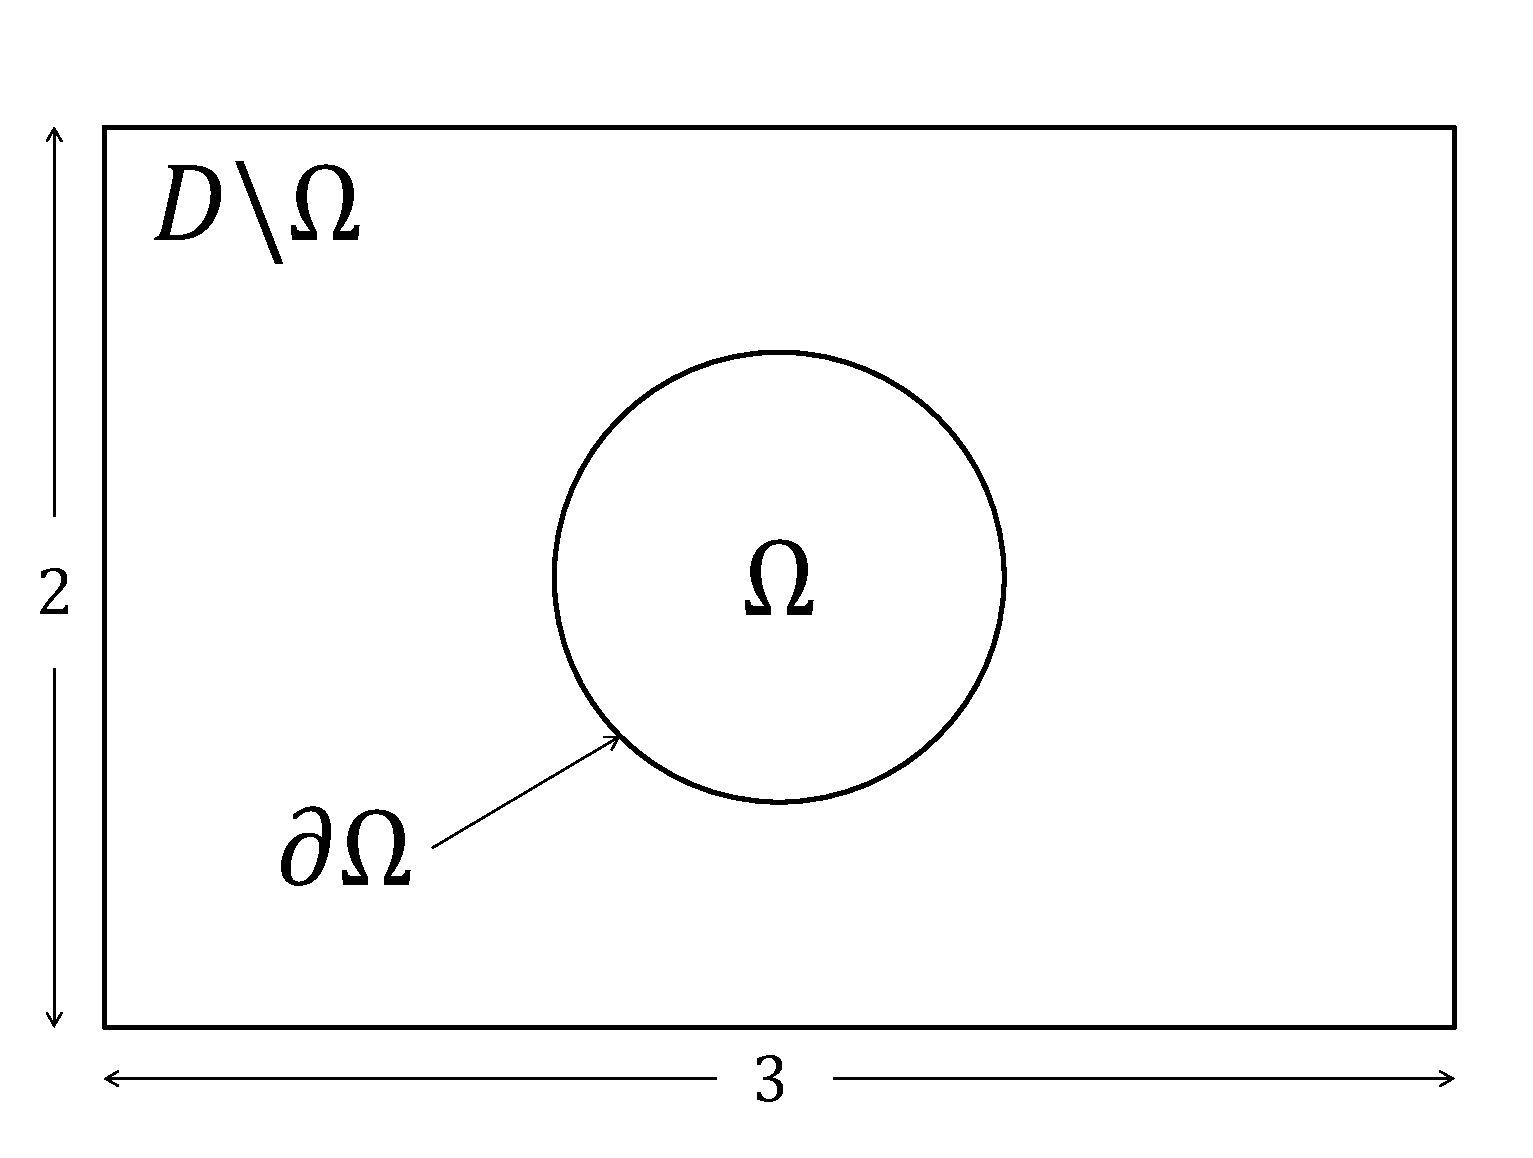
\includegraphics[width=\linewidth]{level_set_circle_domain_050.eps}
		}
	\end{tabularx}
	\caption{The zero level set isolevel of the level set function, $\partial \Omega = \Gamma_{\phi=0}$, in \ref{fig:level_set_circle_func_1} divides the fixed mesh grid into different phase regions in \ref{fig:level_set_circle_domain_1}, where each phase may represent a different material or a different physics.}
	\label{fig:level_set_circle_description}
\end{figure}

To illustrate the differences in the geometry representation between the density and level set methods, consider the ``solid-void'' structural optimization problem presented in Figure \ref{fig:structural_compliance_setup}, where the objective is to minimize the structural compliance by changing the material layout, subject to a maximum volume fraction of 0.5 for the solid phase. The results for both the density and level set approaches are shown in Figure \ref{fig:structural_compliance_comparison}. Notice both designs generate similar truss-like geometries. Figure \ref{fig:structural_compliance_comparison_SIMP} shows how the density method represents the interface between the solid and void materials as intermediate ``grey'' densities, while the level set method in Figure \ref{fig:structural_compliance_comparison_XFEM} describes the geometry by cutting the elements.
%
\begin{figure}[H]
	\centering
	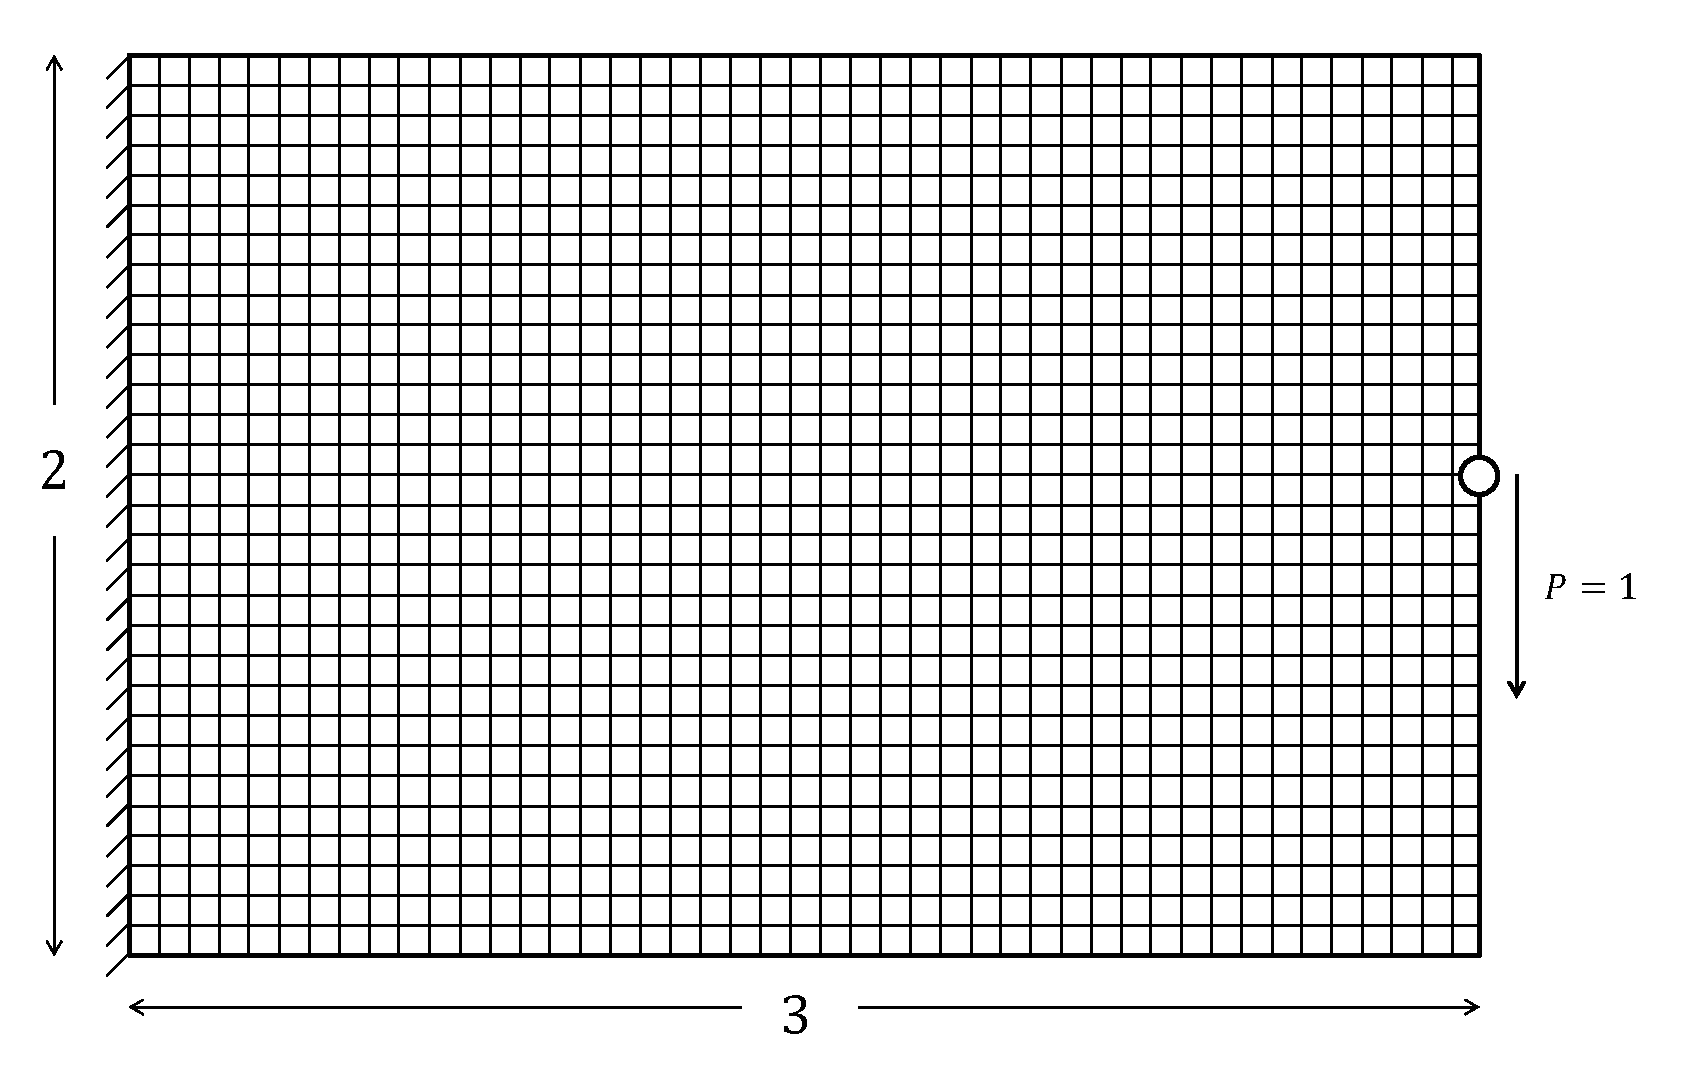
\includegraphics[scale=0.4]{structural_compliance_setup.eps}
	\caption{Setup of a structural topology optimization problem. A mesh of size $3L \times 2L$, with $45 \times 30$ quadrilateral linear elements is anchored to the wall on its left side, and subject to a point load on its right side.}
	\label{fig:structural_compliance_setup}
\end{figure}
%
\begin{figure}[H]
	\centering
	\begin{tabularx}{0.75\linewidth}{X}
		\subfloat[Density method.]{
			\label{fig:structural_compliance_comparison_SIMP}
			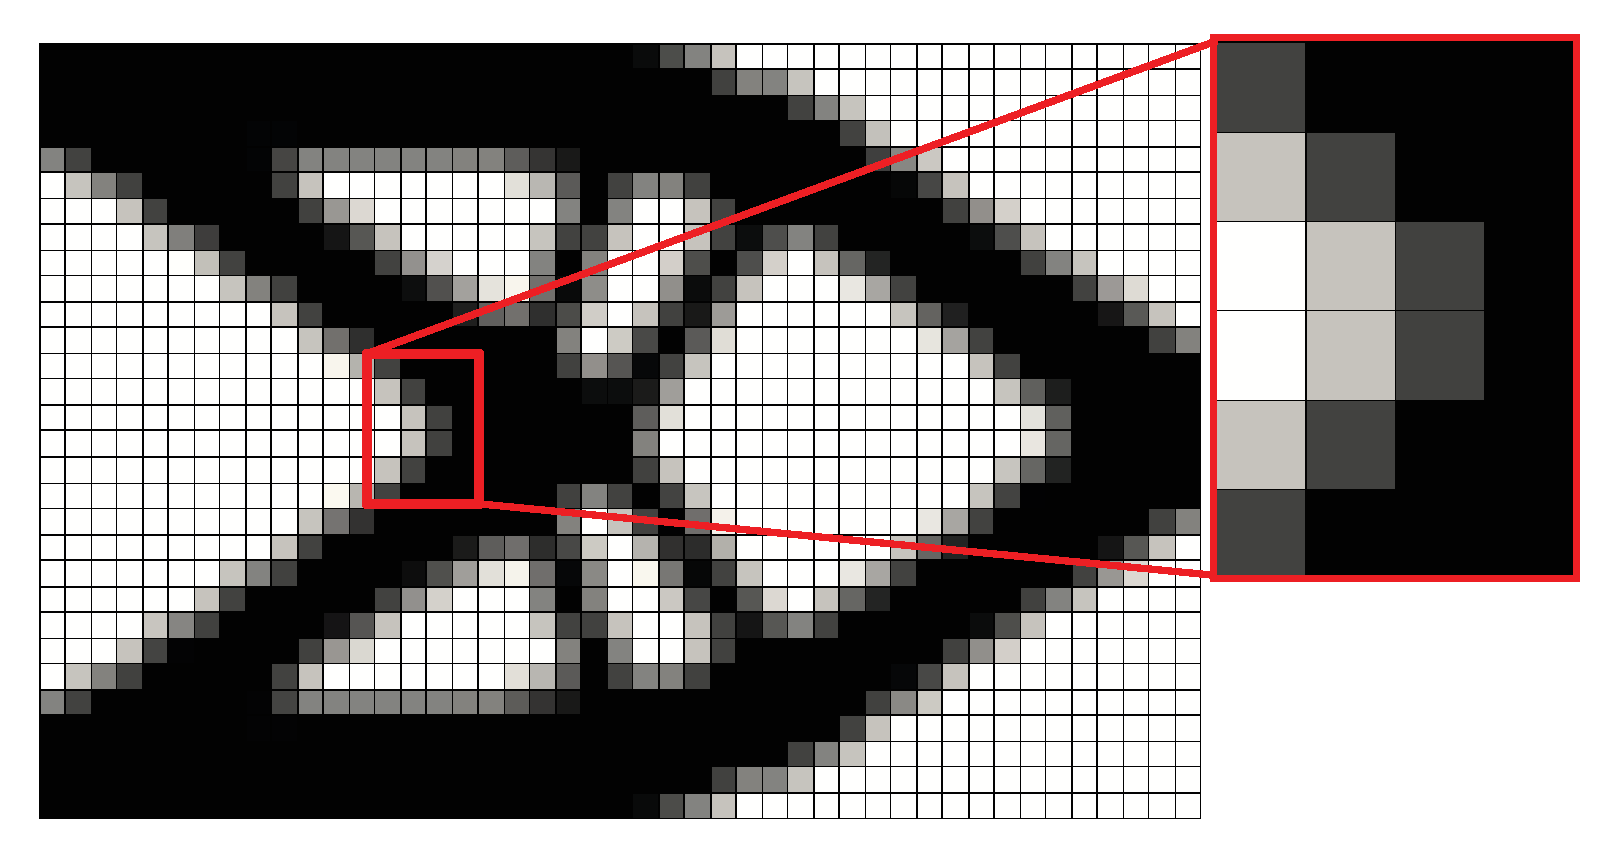
\includegraphics[width=\linewidth]{structural_compliance_comparison_SIMP.eps}
		} \\
		\subfloat[Level set method.]{
			\label{fig:structural_compliance_comparison_XFEM}
			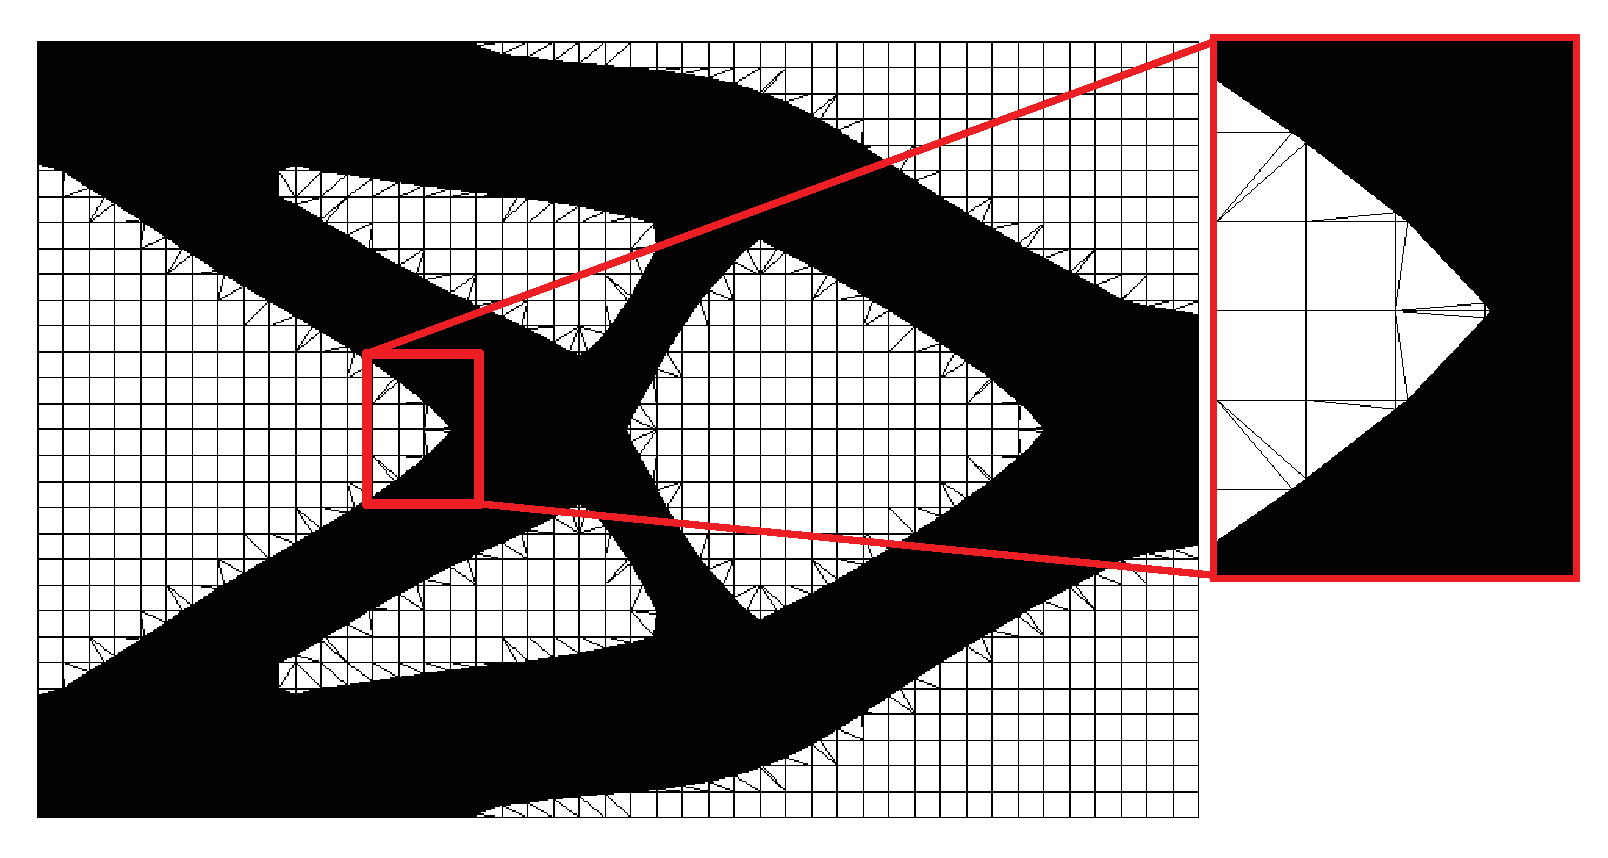
\includegraphics[width=\linewidth]{structural_compliance_comparison_XFEM.eps}
		}
	\end{tabularx}
	\caption{Comparison of the geometry representation of the density and level set methods for a ``solid-void'' structural topology optimization problem.}
	\label{fig:structural_compliance_comparison}
\end{figure}

In the level set method, the material properties of the structural finite elements are interpolated between the void and solid phases, proportional to the volumes of the individual phases. This approach is called Ersatz material interpolation and it is very similar to the interpolation used in density methods. Therefore, it leads to similar issues with regard to enforcing boundary conditions and predicting the physical response along the boundary. The process is illustrated in Figure \ref{fig:ersatz_interpolation}.
%
\begin{figure}[H]
	\centering
	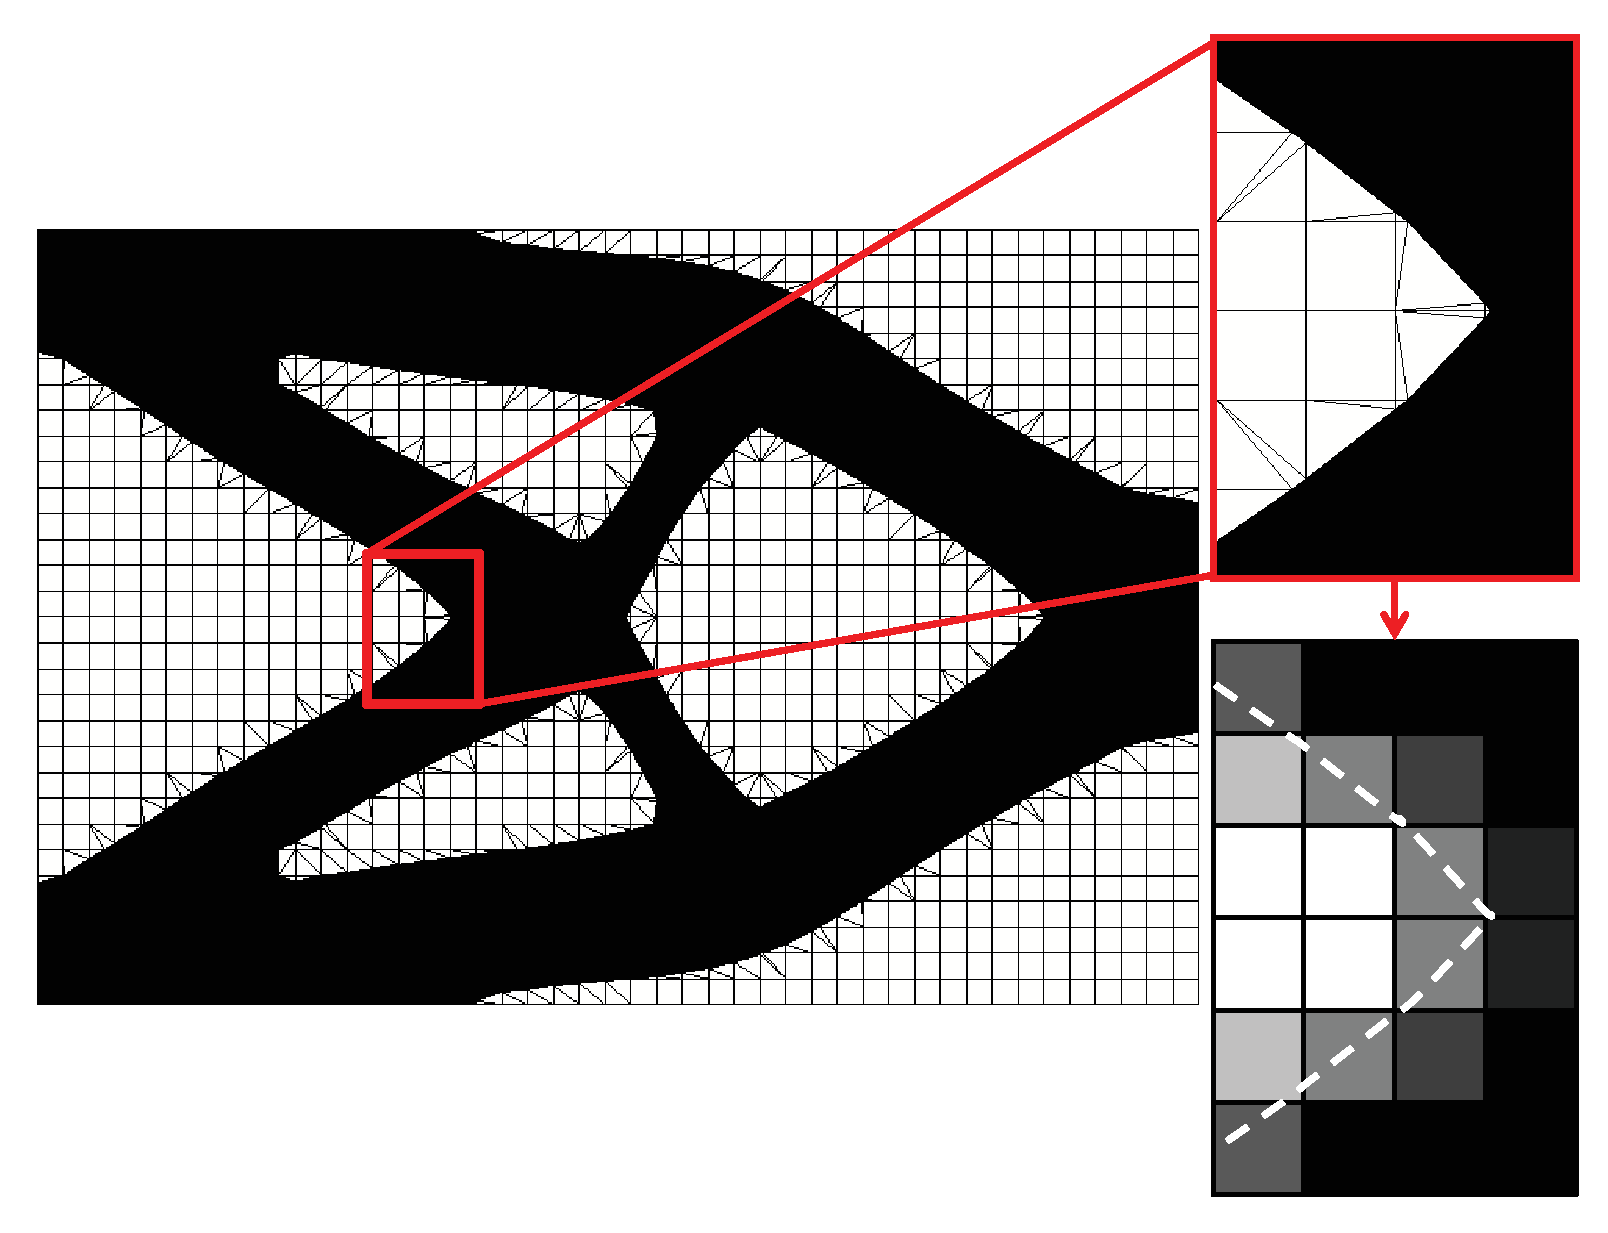
\includegraphics[scale=0.4]{ersatz_interpolation.eps}
	\caption{In an Ersatz material interpolation approach, the material properties of each finite element are interpolated proportional to the volumes of the solid and void phases.}
	\label{fig:ersatz_interpolation}
\end{figure}

An alternative to the Ersatz interpolation is to repeatedly generate new meshes that align with the geometry of the zero level set isolevel, as shown in Figure \ref{fig:remeshing_interpolation}. However, generating an entirely new body fitted
mesh typically suffers from robustness and efficiency, particularly for three dimensional problems. It was also shown by \citep{SMR:00} and \citep{WKG:06} that this method affects the convergence of the optimization process.
%
\begin{figure}[H]
	\centering
	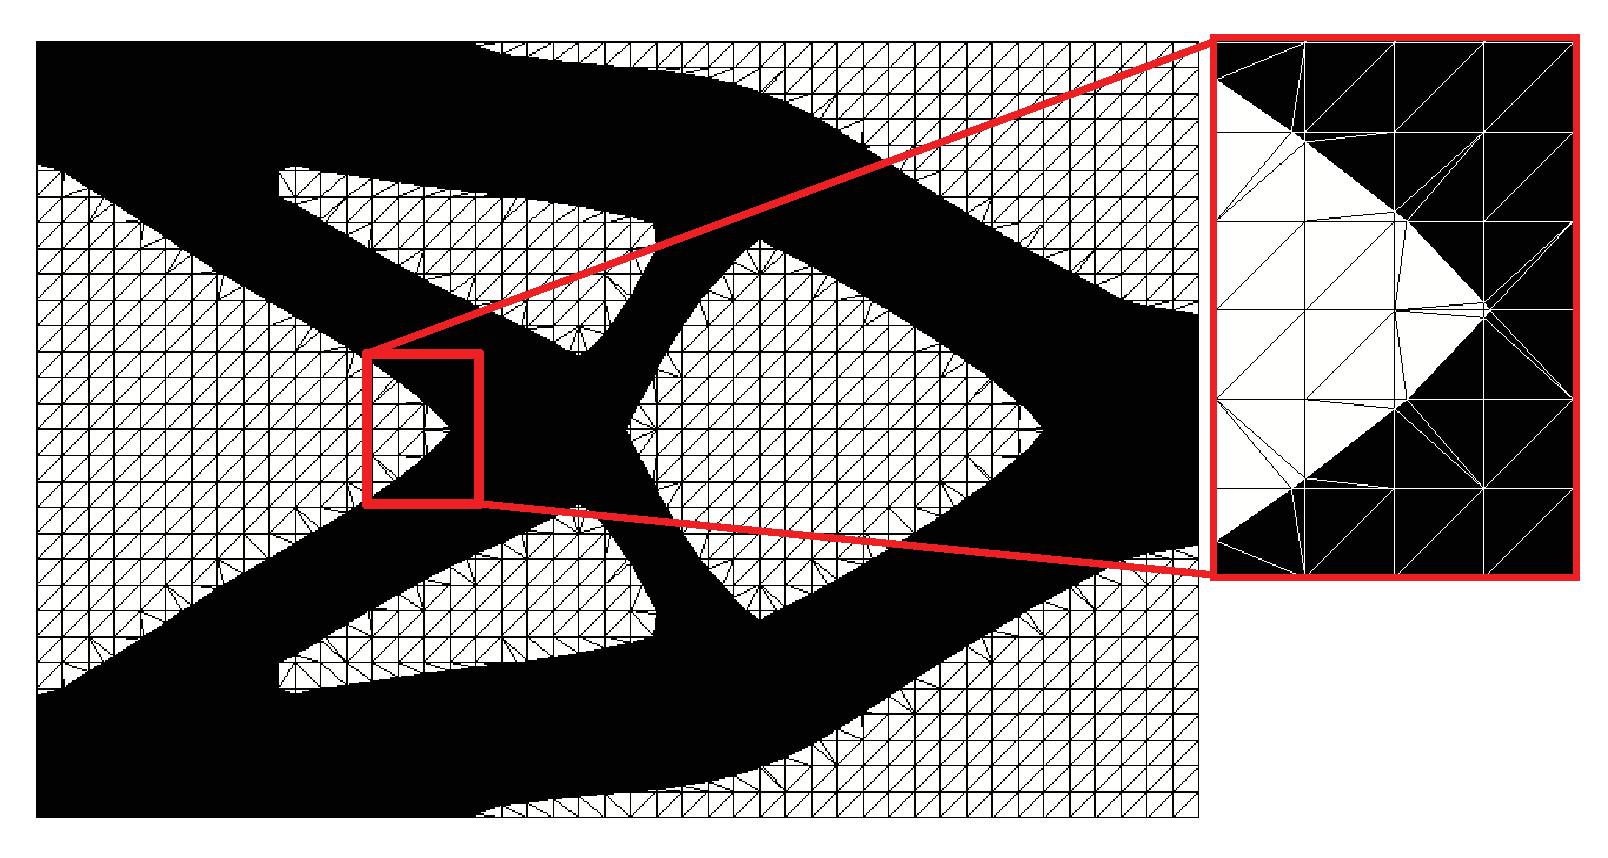
\includegraphics[scale=0.4]{structural_compliance_comparison_remeshing.eps}
	\caption{Remeshing the design domain such that elements align with the zero level set isolevel is an alternative to the Ersatz material interpolation approach.}
	\label{fig:remeshing_interpolation}
\end{figure}

Another approach is used by the XFEM (Section \ref{sec:intro_xfem}). The XFEM is an immersed boundary technique that works on fixed grids, and decomposes the cut elements into subdomains and interfaces that it uses for integration, as shown in Figure \ref{fig:XFEM_interpolation}.
%
\begin{figure}[H]
	\centering
	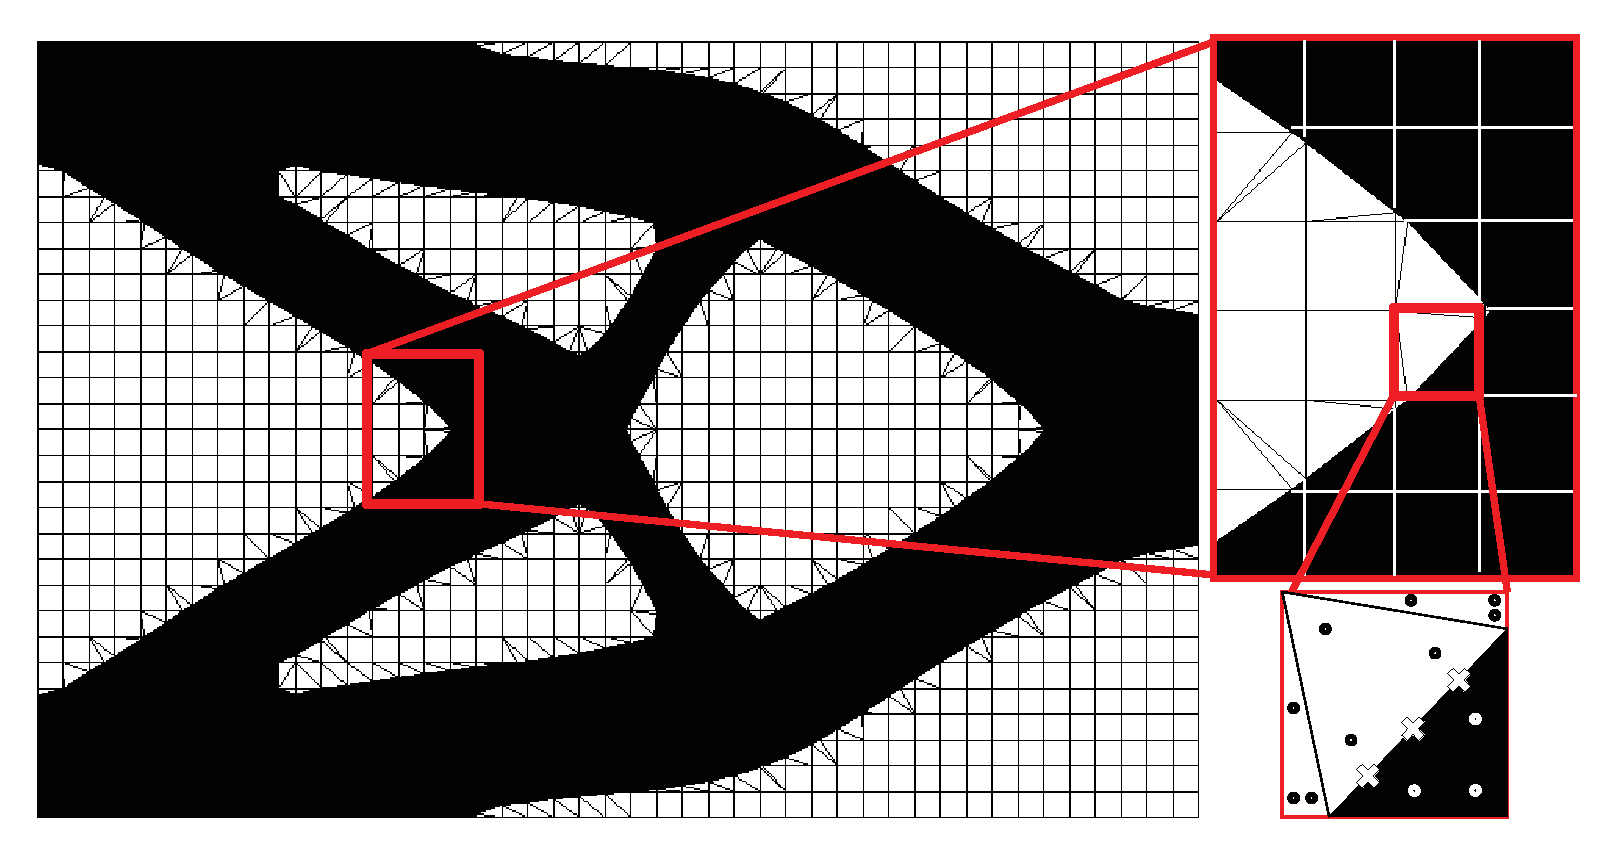
\includegraphics[scale=0.4]{XFEM_interpolation.eps}
	\caption{In the XFEM, the elements cut by the zero level set isolevel are divided into subdomains and interfaces for integration. Circles represent the abscissae for the subdomains, while crosses represent the abscissae for the interface integration.}
	\label{fig:XFEM_interpolation}
\end{figure}

The XFEM enriches the finite element solution space allowing for discontinuities (see Sections \ref{sec:discretization} and \ref{sec:computational-considerations} for details). In this thesis proposal, we will use a Heaviside enrichment strategy, which allows for solution fields with discontinuities $C^{-1}$.

As the topology of the level set function changes, it will occur that a phase subdomain is small enough to cause numerical instabilities in the system, and not lead to convergence. Several approaches have been studied in the literature to try and ameliorate this issue. \citep{LMD+:13} introduced a preconditioner that scales the solution space proportional to the areas of the subdomains. \citep{BH:12,SW:14,SRG+:14} used a ghost penalty formulation to smooth the gradients of the solution at the facets of the cut elements. Both approaches presented favorable results for two dimensional diffusion and incompressible Navier-Stokes flow problems.

Perimeter or curvature measures can be computed at the level set interface using the XFEM. These measures can be introduced into the optimization problem in order to provide a global shape control feature, and prevent the appearance of small floating particles \citep{MM:13}.

This thesis proposal will analyze the characteristics of the proposed LSM-XFEM method as follows:

\begin{enumerate}
	\item \citep{MM:13} studied the XFEM decomposition of the cut elements into subdomains, and the application of multiple enrichment levels in two dimensional problems. Our first hypothesis is that the same approach used by \citep{MM:13} can be extended to three dimensions. Section \ref{sec:a_complete_methodology_for_the_implementation_of_XFEM_inclusive_models} studies the algorithmic details of the approach, and the robustness of the method to describe complex three dimensional geometries using the level set method.

	\item The next question is whether the method can accurately describe the physics at the phase interface without extensive mesh refinement. If so, does it provide an advantage over the interface description provided by the density methods? There are several approaches to approximate the solution at the interface of the level set field, as described in Section \ref{sec:intro_xfem}. We will study the application of stabilized Lagrange multipliers in Section \ref{sec:density_and_level_set_XFEM_schemes_for_topology_optimization_of_3D_structures}, and of the Nitsche method in Section \ref{sec:level_set_XFEM_topology_optimization_of_3D_navier_stokes_and_scalar_transport_problems}.

	\item If the framework can describe complex geometries generated by a level set field, as well as accurately represent the physics at the phase interface, how does it fare overall against density approaches? Section \ref{sec:density_and_level_set_XFEM_schemes_for_topology_optimization_of_3D_structures} applies the framework to three dimensional structural problems, and provides a comprehensive comparison against density methods. The objective is to study convergence rates of the optimization problems, shape control of the optimized geometries, postprocessing capabilities of the methods to generate manufacturable designs, and the effects of providing different initial designs to the optimization process. The hypothesis is that the framework provides a better description of the geometry and material distribution than density methods, and therefore requires coarser meshes which leads to faster computations. Furthermore, it provides the capability to extract surface meshes directly from the level set function and manufacture the designs using three dimensional printing. This feature would be promising for rapid-prototyping.

	\item  In section \ref{sec:preconditioner}, we will expand the scaling preconditioning scheme to structural problems. The preconditioner was previously studied for two dimensional heat conduction problems. The scaling should ameliorate the effects that small intersection regions cause to the solution. In section \ref{sec:level_set_XFEM_topology_optimization_of_3D_navier_stokes_and_scalar_transport_problems}, we will study an alternate approach, the face-oriented ghost-penalty, and its effects on incompressible Navier-Stokes flows. This penalty formulation has been studied in the literature for diffusion and incompressible Navier-Stokes problems, and our hypothesis is that it can be applied in our optimization framework to ensure convergence for three dimensional problems.

	\item Once we can ensure convergence of the solution, the framework should be able to solve a broad range of design engineering problems. In this thesis proposal, we will study structural, incompressible Navier-Stokes flow, and scalar transport problems. These physics will help understand the characteristics, and the capability of the method to be applied to real-world engineering problems. Structural problems are studied in Section \ref{sec:density_and_level_set_XFEM_schemes_for_topology_optimization_of_3D_structures}. Incompressible Navier-Stokes and scalar transport problems are studied in \ref{sec:level_set_XFEM_topology_optimization_of_3D_navier_stokes_and_scalar_transport_problems}.

	\item Controlling the shape of the optimized geometry is important in manufacturing. The effects of using a smoothing filter for the level set field (see Section \ref{sec:intro_level_set_method}) will be studied in Section \ref{sec:feature-size-control}. This filter will also be compared against the density filter (see Section \ref{sec:smoothing_filter}) as a way of controlling the minimum feature size. Regularization techniques applied to the level set interface, such as measuring the curvature and perimeter, may cause different optimized geometries to emerge. The use of these measures and its effects on the finalized design will be studied in Section \ref{sec:topology_optimization_approaches_for_the_curvature_minimization_of_level_set_isocontours}.
\end{enumerate}

The studies proposed above will help us understand the characteristics and capabilities of the framework. The final step is to use this knowledge to study the method in the context of a real-world problem that requires the modeling of a three dimensional incompressible Navier-Stokes flow with a scalar transport field in Section \ref{sec:modeling_of_multiple_scalar_transport_fields_for_an_atomic_layer_deposition_machine}.

The specific objectives of this thesis proposal are then:
\begin{inparaenum}[(i)]
	\item To generate a robust LSM-XFEM topology optimization scheme;
	\item To compare the LSM-XFEM optimization scheme with traditional homogenization methods, such as SIMP, and study the advantages and disadvantages of our formulation;
	\item and to explore the characteristics of the methodology through cases studies in selected applications.
\end{inparaenum}

The layout of this thesis proposal is as follows: Section \ref{sec:introduction} presented the motivation and goals of the study, Section \ref{sec:background} presents an overview of the concepts required to understand this work, Section \ref{sec:a_complete_methodology_for_the_implementation_of_XFEM_inclusive_models} presents the algorithm to implement an XFEM framework in software, Section \ref{sec:density_and_level_set_XFEM_schemes_for_topology_optimization_of_3D_structures} presents the application of the methodology in structural problems, and compares the results to density approaches, Section \ref{sec:level_set_XFEM_topology_optimization_of_3D_navier_stokes_and_scalar_transport_problems} presents the application of the method to incompressible Navier-Stokes flows and scalar transport problems, Section \ref{sec:topology_optimization_approaches_for_the_curvature_minimization_of_level_set_isocontours} studies regularization techniques to improve the manufacturing of the design, Section \ref{sec:modeling_of_multiple_scalar_transport_fields_for_an_atomic_layer_deposition_machine} uses the methodology for a real-world design engineering problem. Finally, Sections \ref{sec:remaining_work} and \ref{sec:main_conclusions} show the remaining work and conclusions of this thesis proposal.

% -----------------------------------------------------------------------------

\chapter{Background}
\label{sec:background}

This chapter presents a brief overview on topology optimization, the level set method, and finite element methods. The information presented in this chapter is sufficient such that the reader can understand the framework in which the thesis is developed, but it is not comprehensive. References are provided for the reader who wishes to see more details on the topics.

% -----------------------------------------------------------------------------

\section{Optimization}
\label{sec:optimization}

An optimization problem is a problem in which you seek to find the best solution from the set of all feasible solutions. There are two categories of optimization problems, and their classification depends on whether the problem variables are continuous or discrete. In this work, we will focus on optimization problems with continuous variables. An optimization problem with discrete variables is known as a combinatorial optimization problem, and the reader is directed to \citep{NW:88} for a review.

The standard form for an optimization problem with continuous variables is:
%
\begin{equation}
\label{eq:optimization_standard_form}
	\begin{aligned}
		&\min_{\mathbf{s}} \mathcal{F}(\mathbf{s}, \mathbf{u}(\mathbf{s})), \\
		&\text{s.t.\,}
		\begin{cases}
			\mathbf{s}, & \text{subject to design constraints}  \ \mathcal{G}_j \leq 0 \text{,}\\
			\mathbf{u}, & \text{solves} \ W= 0 \ \text{for a given $\mathbf{s}$,}
		\end{cases}
	\end{aligned}
\end{equation}
%
where the goal is to minimize some objective functional $\mathcal{F}$ with respect to the vector of design variables $\mathbf{s}$. The design variables are subject to the $j$-th design constraint $\mathcal{G}_j$, which are enforced as an inequality problem. In general, the objective and constraints depend on the optimization variables, $\mathbf{s}$, and the state variables, $\mathbf{u}$. These state variables, $\mathbf{u}$, satisfy the weak form of the equilibrium equation $W$, which is enforced as an equality constraint. By convention, Equation \ref{eq:optimization_standard_form} defines a minimization problem. Maximization problems are handled by placing a negative sign on the objective functional $\mathcal{F}$.

% -----------------------------------------------------------------------------
% Optimization algorithms

There are several optimization algorithms available to update the design variables. For structural optimization problems with non-trivial and multiple constraints, the Method of Moving Asymptotes (MMA) \citep{Svanberg:87}, and its globally convergent counterpart, the Globally Convergent Method of Moving Asymptotes (GCMMA) \citep{Svanberg:02} have become the algorithms of choice. The work of this document will focus on the GCMMA algorithm. For a reference on more advanced mathematical tools, such as thr Sequential Quadratic Programming (SQP), the Sparse Nonlinear OPTimizer (SNOPT) \citep{GMS:02}, or the Interior Point OPTimizer \citep{WBL:06}, the reader is referred to the work of \citep{SM:13}.

% -----------------------------------------------------------------------------
% Design sensititivies

Gradients of the objective functional and design constraints with respect to the design variables are required by the mathematical algorithms specified above. The sensitivities for the optimization problems presented in this document will be computed using the adjoint method \citep{GP:08,YSL:02}.

In the following sections, we will delve into the approaches available to solve the optimization problem.

% -----------------------------------------------------------------------------

\section{Topology optimization}
\label{sec:intro_topology_optimization}

Topology optimization is a type of optimization problem in which you seek the optimal geometry and/or material layout of a body within a given design domain $D$. For example, mathematically we can formulate the following generic topology optimization problem: 
%
\begin{equation}
\label{eq:topology_optimization_generic}
		\min_{\mathbf{s}} \int_{\Omega} f \left( \mathbf{s(\mathbf{x})} \right) d{\Omega}
\end{equation}
%
which, analogous to Equation \ref{eq:optimization_standard_form} is subject to design constraints and equilibrium equations. The goal of the optimization problem is to minimize some objective functional $\int_{\Omega} f \left( \mathbf{s(\mathbf{x})} \right) d{\Omega}$ over the design domain with respect to the design variables $\mathbf{s(\mathbf{x})}$, where $\Omega$ represents the shape of the design. The optimization problem will set the design variables as ``on'' or ``off'' in order to minimize the design objective, while satisfying the design constraints. We can represent a design variable at a point $i$ as ``on'' by setting $s_{i}=1.0$, and ``off'' by $s_{i}=0.0$. A quick example is described in Figures \ref{fig:structural_compliance_setup} and \ref{fig:structural_compliance_example}. Figure \ref{fig:structural_compliance_setup} shows the setup for a topology optimization problem with an objective of minimal compliance and subject to a maximum volume fraction of $0.5$ for the solid phase. Figure \ref{fig:structural_compliance_example} shows the changes in the design, where the design variables at the elements are represented as ``on'' (black) or ``off'' (white) or in-between (grey).
%
\begin{figure}
	\centering
	\begin{tabularx}{\linewidth}{XX}
		\subfloat[Step 0.]{
			\label{fig:structural_compliance_0}
			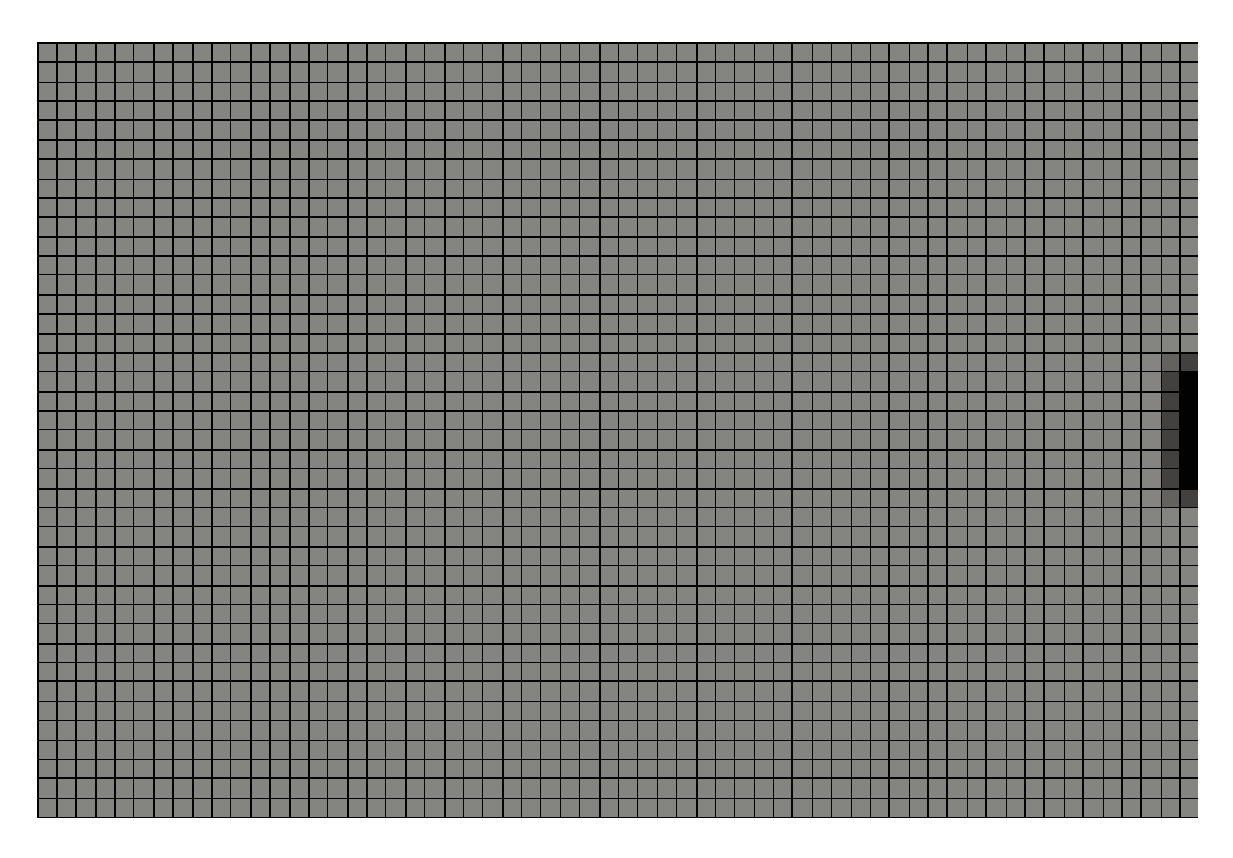
\includegraphics[width=\linewidth]{structural_compliance_0.eps}
		} &
		\subfloat[Step 5.]{
			\label{fig:structural_compliance_5}
			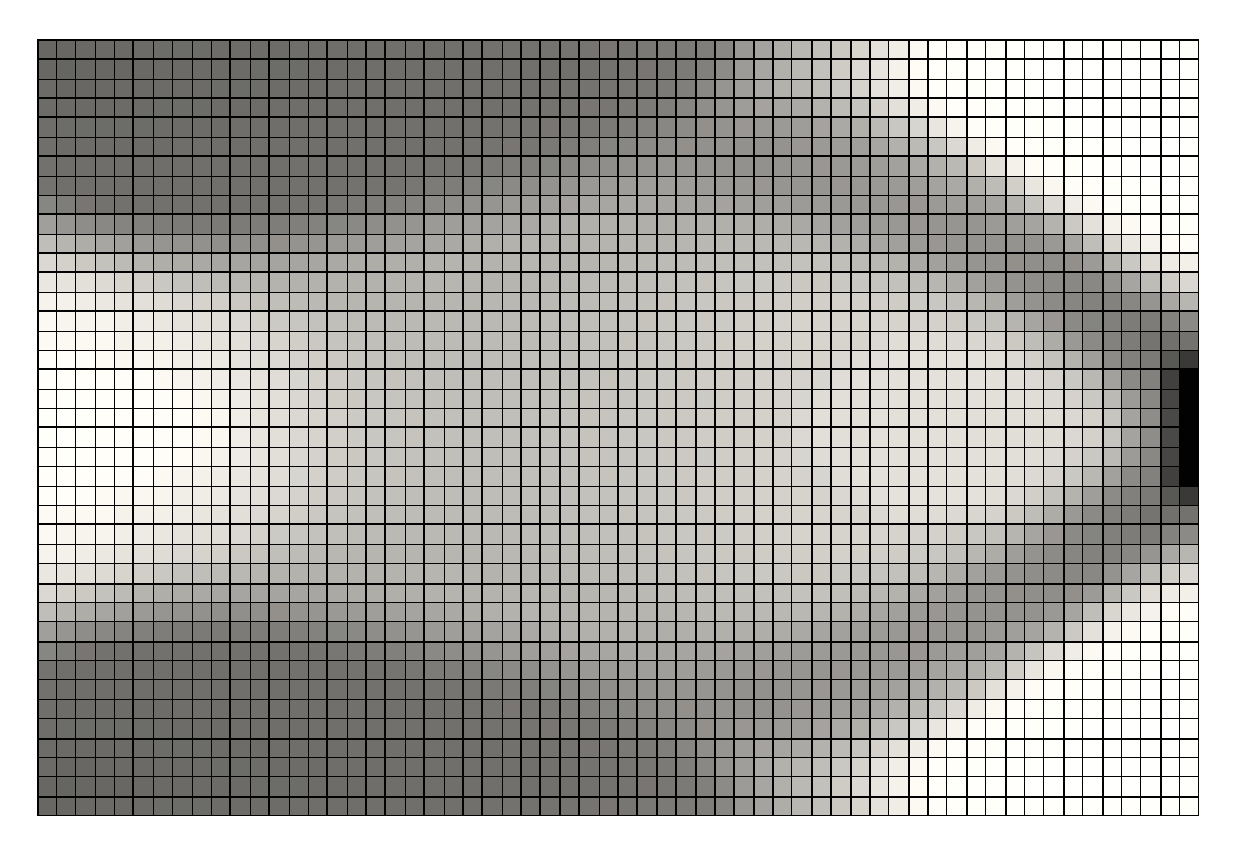
\includegraphics[width=\linewidth]{structural_compliance_5.eps}
		} \\
		\subfloat[Step 10.]{
			\label{fig:structural_compliance_10}
			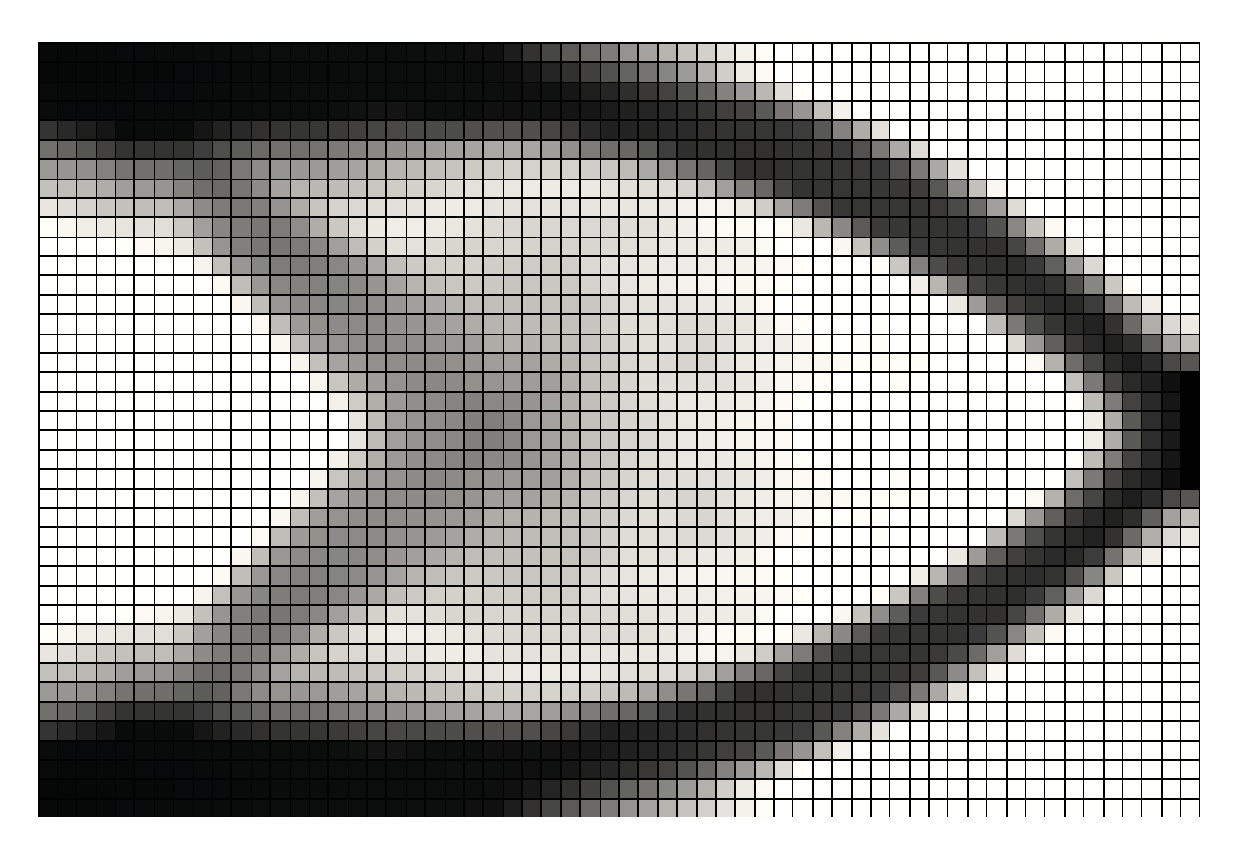
\includegraphics[width=\linewidth]{structural_compliance_10.eps}
		} &
		\subfloat[Step 15.]{
			\label{fig:structural_compliance_15}
			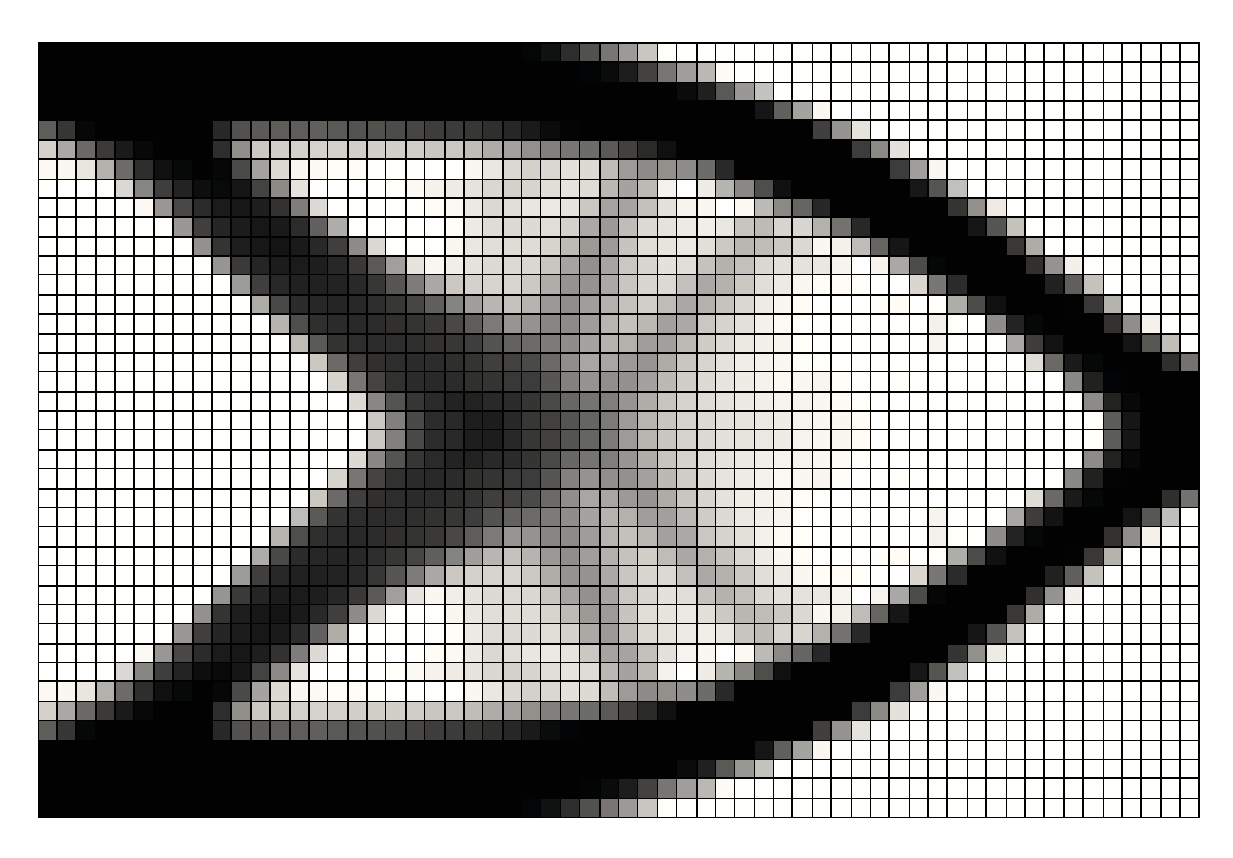
\includegraphics[width=\linewidth]{structural_compliance_15.eps}
		} \\
		\subfloat[Step 25.]{
			\label{fig:structural_compliance_25}
			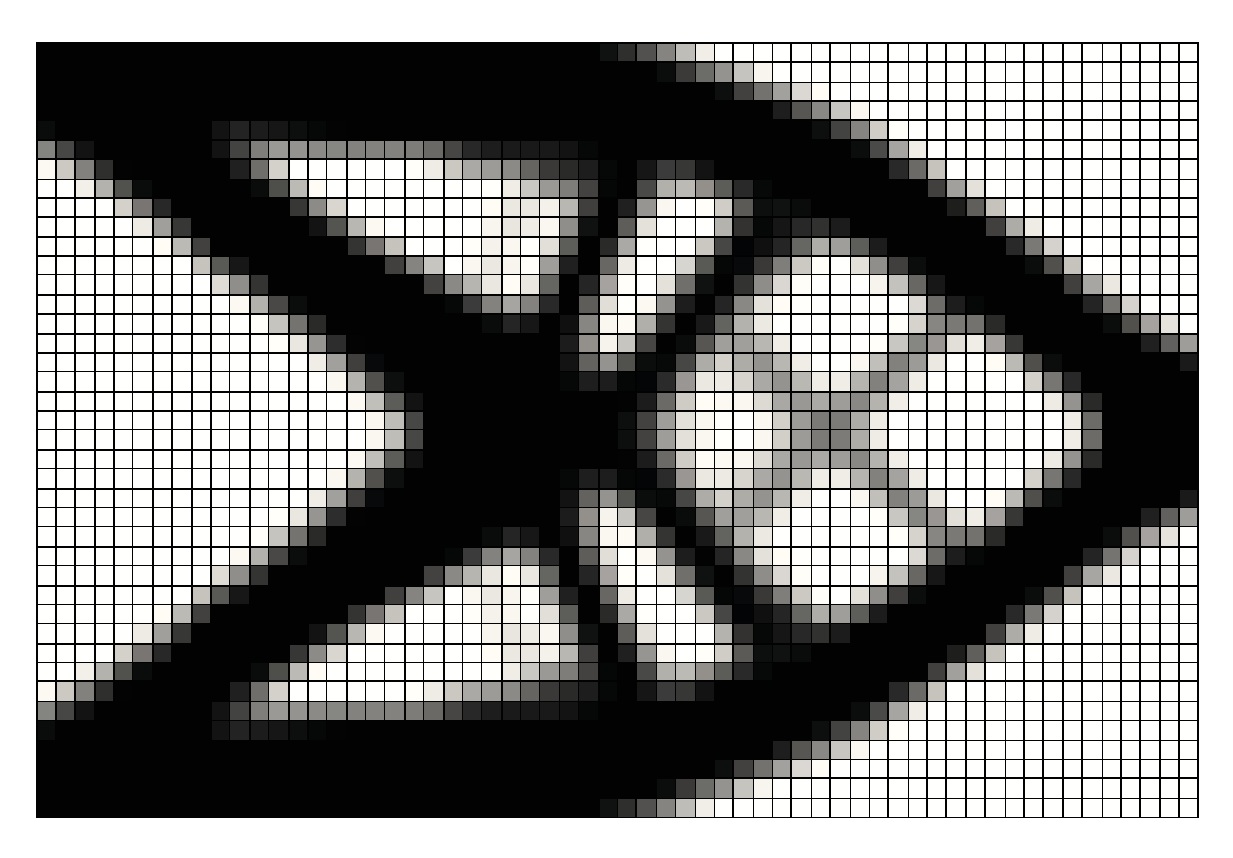
\includegraphics[width=\linewidth]{structural_compliance_25.eps}
		} &
		\subfloat[Step 50.]{
			\label{fig:structural_compliance_50}
			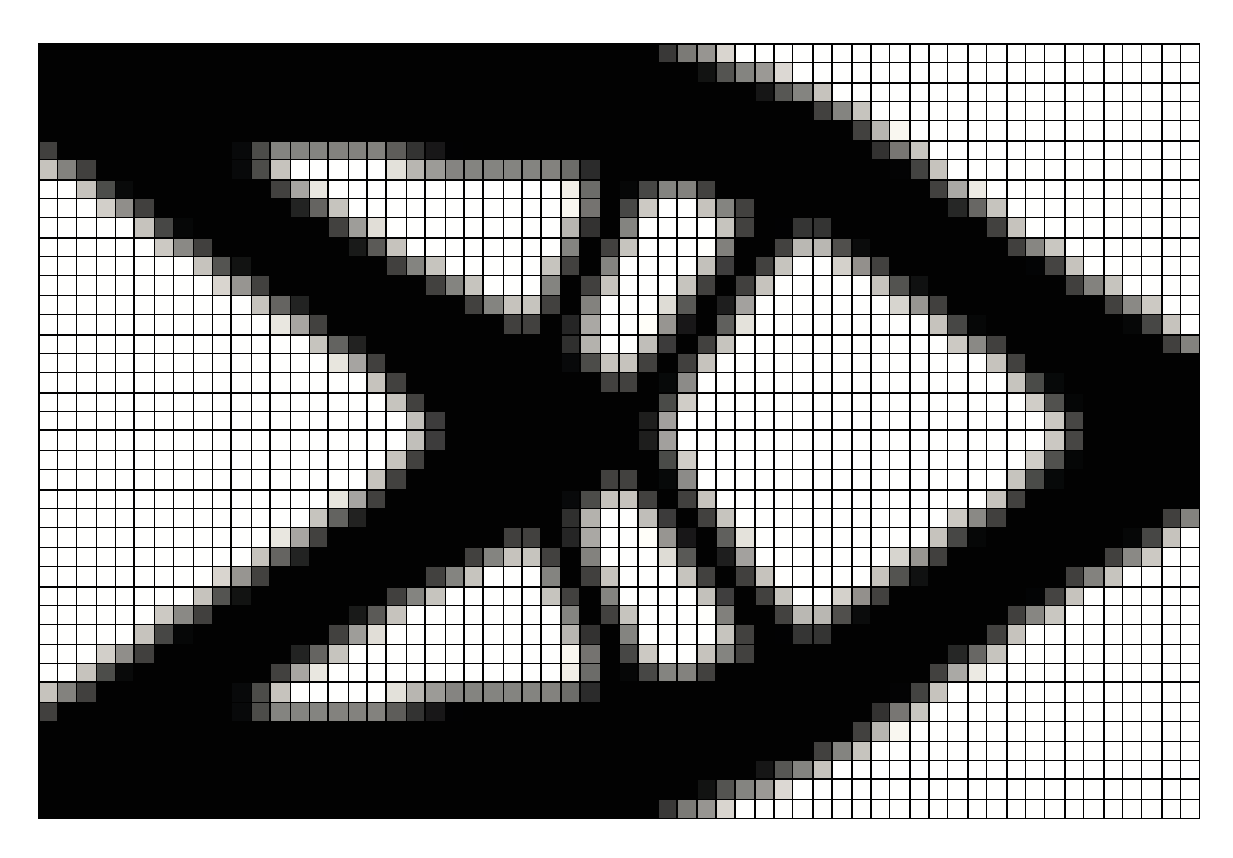
\includegraphics[width=\linewidth]{structural_compliance_50.eps}
		} \\
	\end{tabularx}
	\caption{Progression of the optimization process. Objective is to minimize compliance subject to a maximum volume fraction of 0.5 for the solid phase.}
	\label{fig:structural_compliance_example}
\end{figure}

Topology optimization provides the ability to create designs that are not always intuitive, or to improve on existing designs. Topology optimization methods were initially developed to create conceptual designs in the early stage of the design process \citep{BS:03,Rozvany:09}. It is interesting to note that the earliest recorded paper on topology optimization dates back to 1904, with the work of Australian inventor Michell in the derivation of optimality criteria for least-weight layout of trusses \citep{Michell:04}. And while topology optimization focused for decades on structural design, it has recently found its application in a wide range of physical disciplines \citep{BLO+:05} including acoustics \citep{FAN+:04}, wave propagation \citep{Frenzel:04}, electromagnetics \citep{LGD:09,SHW+:08} and optics \citep{BHF+:04,KOY:05}. For a more detailed review on topology optimization, please refer to \citep{BS:03,EO:01}.

% \footnote{\label{fn:topopt_app}
% At this point, the author recommends you take out your iPhone and iPad and download the best (and ahem... only) structural topology optimization application in the market, TopOpt, from the DTU Mechanical Engineering department. Use this as an exercise to reinforce the concepts explained in this paragraph. Start the application and define a structural problem adding boundary conditions and loads. Before you start the optimization process, try and think of what a good design would be for the problem at hand. Do this for several problems, and compare your intuition to the results of the optimization application. You may realize how helpful topology optimization can be for creating structures with the optimal design.}

% -----------------------------------------------------------------------------
% \subsection{Structural topology optimization}

Structural topology optimization, specifically topology optimization of continuum structures, is in its mathematical nature one of the most challenging optimization problems \citep{BS:03}. However, in 1988, \citep{BK:88} introduced their seminal paper on the homogenization method. In this method, the design domain is assumed to be formed by a material with micro-scale voids, and the topology optimization problem seeks the optimal porosity of the porous medium in order to minimize the objective functional. Due to its effectiveness and simplicity, homogenization-based methods found a lot of applications in structural design, and quickly became the main approach in structural topology optimization \citep{Bendsoe:89}. The homogenization method works by transforming the structural optimization problem into a standard nonlinear program where the design variables are coefficients of the underlying governing equation, and therefore is capable of producing internal holes in the design domain without \textit{a priori} knowledge of them.

% -----------------------------------------------------------------------------

\section{Density topology approaches}
\label{sec:density_topology_approaches}

In 1989, \citet{Bendsoe:89,ZR:91} introduced the most popular of homogenization methods, the ``solid isotropic material with penalization'' (SIMP). In SIMP, the design variables represent the artificial densities, $\rho\left(\mathbf{x}\right)$, of a group of elements in a fixed finite element grid (our design domain $D$) and their material properties are parameterized in terms of a set of material interpolation functions such that intermediate properties are penalized. The typical approach is to assume a value of $\rho=1.0$ represents solid material, while $\rho=0.0$ represents void.

% -----------------------------------------------------------------------------

\subsection{Smoothing filter}
\label{sec:smoothing_filter}

An additional numerical scheme is necessary to smear out numerical instabilities. This is referred to as the filtering method \citep{Sigmund:01a,Sigmund:01b}. For example, in structural topology optimization, the density, rather than being equal to a single variable, can be computed from a linear smoothing filter as follows:

\begin{equation}
	\label{eq:smoothing_filter_SIMP}
	\tilde{\rho}\left(\mathbf{s}\right)=\frac{\sum_{i=1}^{E}w_{i}s_{i}}{\sum_{i=1}^{E}w_{i}}
\end{equation}

with

\begin{equation}
	\label{eq:weight_SIMP}
	w_{i}=\max \left( 0, r_{\rho} - \Vert \mathbf{x}_i - \mathbf{x} \Vert \right)
\end{equation}

where $s_{i}$ is equivalent to an artificial density $\rho$ at a point $\mathbf{x}_{i}$, $\mathbf{x}_{i}$ is the location of the node at which the design variable $i$ is defined, $\tilde{\rho}\left(\mathbf{s}\right)$ is the density at a point $\mathbf{x}$,  $w_{i}$ is the factor of point $\mathbf{x}$ with respect to the design variable $i$, $r_{\rho}$ is the filter radius, and $E$ is the number of elements in the design domain.

The filter in Equation \ref{eq:smoothing_filter_SIMP} prevents the formation of features smaller than $r_{\rho}$, and serves as a minimum feature size control. However, this comes at the cost of forming intermediate densities along the material interface. Methods for smearing out intermediate densities have been proposed by \citep{FJP:05,Sigmund:07,SS:01a}. \citep{GPB:04} proposed a density projection method to reduce the volume occupied by material with intermediate densities. This projection is based on a smoothed Heaviside function and applied to the densities as follows:
%
\begin{equation}
\label{eq:heaviside_density}
		\hat{\rho}\left(\tilde{\rho}\right) = 1-e^{-\beta\tilde{\rho}}+\tilde{\rho}e^{-\beta}
\end{equation}
%
where $\hat{\rho}$ is the projected density, and the parameter $\beta \ge 0$ controls the crispness of the projection. Notice that for $\beta=0$ we recover the original density $\hat{\rho}=\tilde{\rho}$. As we increase $\beta$, more and more intermediate densities are penalized towards the value of 1.0, as shown in Figure \ref{fig:density_heaviside}. Note, however, that if the objective and/or constraints of the optimization problem find the intermediate densities to be benefitial, the optimization algorithm will ignore the effects of this projection scheme. The reader is referred to \citep{GPB:04,GAH:11,Sigmund:07,XCC:10,WLS:11} for more details on projection schemes.
%
\begin{figure}
	\centering
	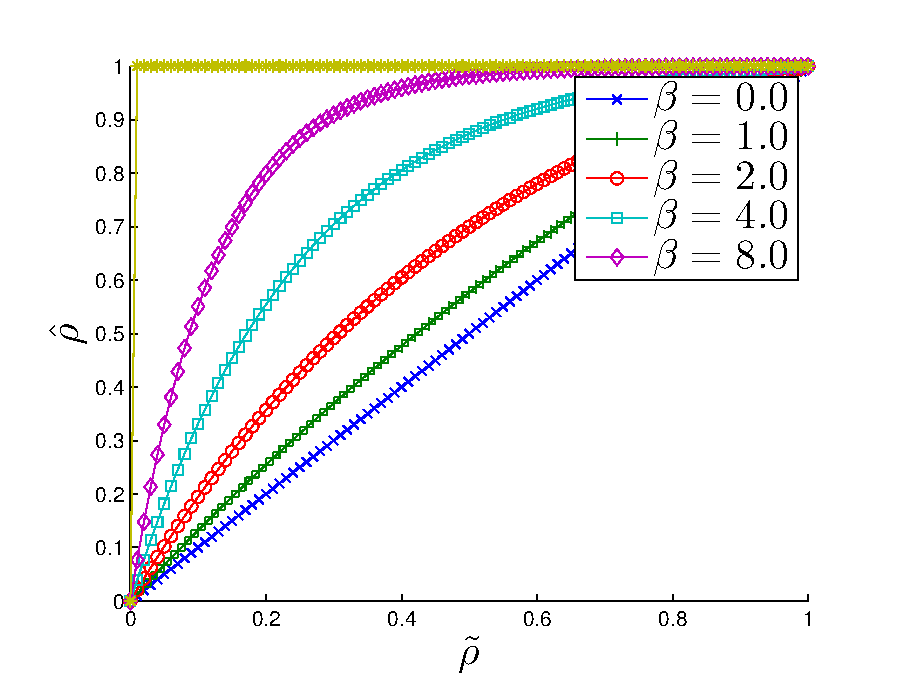
\includegraphics[scale=0.75]{density_heaviside.eps}
	\caption{The density Heaviside projection for various magnitudes of $\beta$.}
	\label{fig:density_heaviside}
\end{figure}
%
In structural topology optimization, it is important to model the relation between density and stiffness. SIMP models the stiffness proportional to the density in the power $p$, where $p > 1$ \citep{BS:99}, in order to guarantee a well-posed optimization problem \citep{BS:99}. The structural stiffness for a ``solid-void'' problem can then be formulated as:
%
\begin{equation}
\label{eq:structural_stiffness}
		E\left(\mathbf{x}\right) = \hat{\rho} ^ p E_{0}
\end{equation}
%
where $E_{0}$ is the initial structural stiffness of the material. Typically, the parameter $p$ is set to 1, and then increased as the optimization progresses \citep{RZS:94}; this is the so-called continuation method \citep{SP:98}. It was shown that if one uses $p > 3$, we recover a black-and-white binary-like material distribution \citep{BS:03}. That is why the density approach has been referred to as a \textit{pixelated} geometric model.

% -----------------------------------------------------------------------------
% Multimaterial SIMP
% \subsection{Multimaterial SIMP}

The SIMP method can be expanded to model a multi-material optimization problem. For example, applying a ``rule of mixture'', we can model a two-phase material in structural topology optimization by modifying Equation \ref{eq:structural_stiffness} as:

\begin{equation}
	\label{eq:two_phase_stiffness}
	E\left(x\right) = \hat{\rho} ^ p E_{A} + \left( 1 - \hat{\rho} ^ p \right) E_{B}
\end{equation}

where $E_{A}$ represents the stiffness of material ``A'', and $E_{B}$ represents the stiffness of material ``B''. Notice that if we model the material phase ``B'' as void, and set $E_{B}=0$ we recover the original equation from \ref{eq:structural_stiffness}. This method uses a single design variable field to model up to two different materials.

For a three-phase or more material optimization problem, we require an extended power law interpolation with multiple design variable fields (i.e. $\mathbf{s}_{1}$, $\mathbf{s}_{2}$, etc.), as shown in \citep{WW:04c,PS:14}. In general, the SIMP method requires $\left( n - 1 \right)$ design variable fields for $n$ distinct material phases \citep{WW:04c}.

% -----------------------------------------------------------------------------

\subsection{Density methods applied to fluid dynamics}
\label{sec:intro_density_fluid_dynamics}

Several applications require finding the optimal geometries of systems to improve the performance of internal and external flows \citep{Maute:14}. Adopting the concept of density methods, \citep{BP:03} extended the methodology to fluid related problems. They modeled the influence of a wall or body in the fluid flow by representing it as a body force in the incompressible Navier-Stokes equations as:
%
\begin{equation}
	\label{eq:navier_stokes}
	\rho^{f} \left( \frac{\partial v_{i}}{\partial t} + v_{j} \frac{\partial v_{i}}{\partial x_{j}} \right) = \frac{\partial}{\partial x_{j}} \left( -p \delta_{ij} + \mu^{f} \left( \frac{\partial v_{j}}{\partial x_{i}} + \frac{\partial v_{i}}{\partial x_{j}} \right) \right) + f_{i}
\end{equation}
%
\begin{equation}
	\label{eq:divergence_stokes}
	\frac{\partial v_{i}}{\partial x_{i}} = 0
\end{equation}
%
where $\rho^{f}$ is the fluid density, $v_{i}$ is the velocity along the spatial dimension $i$, $p$ is the fluid mechanical pressure, $\mu^{f}$ is the fluid dynamic viscosity, and $f_{i}$ is the force exerted by the porous media:
%
\begin{equation}
	\label{eq:brinkman_force}
	f_{i} = - \alpha v_{i}
\end{equation}
%
This methodology is referred to as the Brinkman penalization. Similar to structural topology optimization problems, we set the design variables, $\mathbf{s}$, to represent the fluid fraction at a point of the design domain, and set $\mathbf{s}=\gamma=\gamma \left( \mathbf{x} \right)$, where $\left( 0 \le \gamma \le 1 \right)$. Typically, $\gamma = 1$ represents the fluid domain, and $\gamma=0$ represents the solid domain.

The coefficient $\alpha$ can be interpolated from the design variables as:
%
\begin{equation}
	\label{eq:alpha_linear}
	\alpha = \alpha_{max} \gamma
\end{equation}
%
The parameter $\alpha_{max}$ should be large enough such that the term $\mathbf{f}$ in Equation \ref{eq:navier_stokes} sufficiently penalizes the flow to $\mathbf{u}=0$. \citep{KMK:12} set $\alpha_{max}$ to:
%
\begin{equation}
	\label{eq:alpha_max}
	\alpha_{max} = \left( 1 + \frac{1}{Re} \right) \chi
\end{equation}
%
where $Re$ is the Reynolds number, and $\chi$ is set to a very large value, i.e. $10^4$.

However, this linear interpolation causes large gradients in the fluid flow, which cause numerical issues and may lead to the optimization problem converging to a local minimum. \citep{BP:03} introduced a convex interpolation:
%
\begin{equation}
	\label{eq:alpha_interpolation}
	\alpha \left( \mathbf{x} \right) = \alpha \left( \gamma \left( \mathbf{x} \right) \right) = \alpha_{max} + \gamma \left( \alpha_{min} - \alpha_{max} \right) \frac{1 + \alpha_{p}}{\gamma + \alpha_{p}}
\end{equation}
%
Figure \ref{fig:alpha_convex} shows the influence of the perimeter $\alpha_{p}$. In general, we want to choose $\alpha_{p}$ to be as low as possible, but high enough to prevent intermediate porosities from showing up in the optimization process. In the work of \citep{KM:11}, $\alpha_{p}$ was chosen to be 0.01 with favorable results. $\alpha_{min}$ is set to zero, such that at its minimum, $\alpha=0$ recovers the original Navier-Stokes equations.
%
\begin{figure}
	\centering
	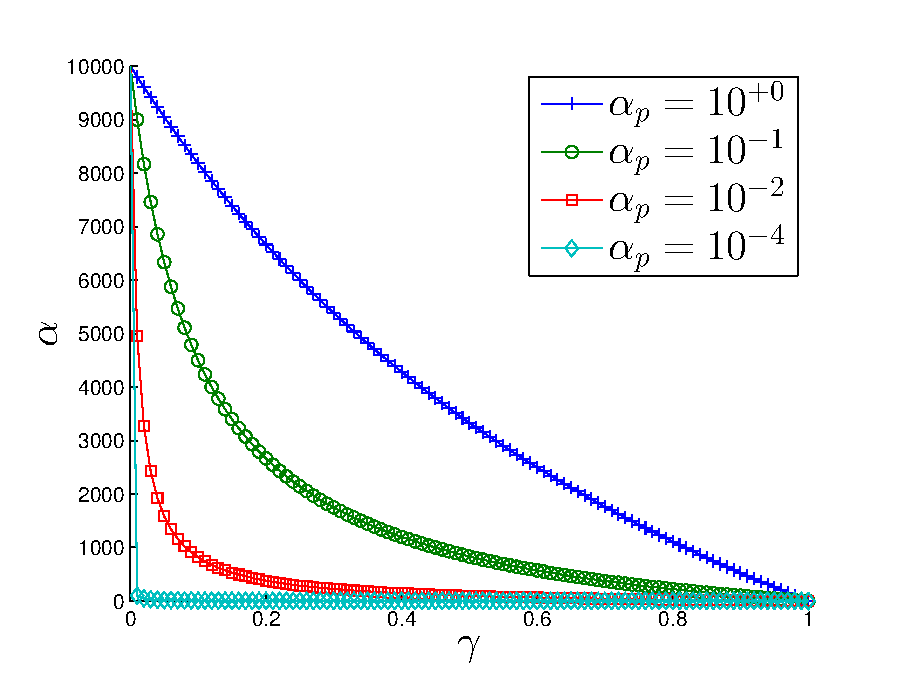
\includegraphics[scale=0.75]{alpha_convex.eps}
	\caption{Influence of the interpolation penalty $\alpha_{p}$.}
	\label{fig:alpha_convex}
\end{figure}
%
For more details on topology optimization of Stokes and Navier-Stokes flows, the reader is referred to \citep{Maute:14}.

% -----------------------------------------------------------------------------

\subsection{Discussion of the SIMP approach}
\label{sec:SIMP_discussion}

The concept of relating some artificial densities to the stiffness in structural problems can be expanded to other physics disciplines. The SIMP method can be used the describe material properties in thermal conductivity, magnetic permeability, porosity, etc.; and therefore, it found its way to a wide range of applications. The method requires a relatively small amount of iterations in order for the optimization problem to converge to an optimal design (at least for ``solid-void'' problems). SIMP has this capability because it operates on the entire design domain and not only on the boundaries; therefore, it does not suffer from localization effects. The approach is also suitable for a wide combination of design constraints, multiple load conditions, and extremely large (often 3D) systems. The educational article by \citet{Sigmund:01b} detailing a 99-line SIMP-code implemented in Matlab, as well as his web-based topology optimization program \citep{TS:01}\footnote{The software is now available on iOS phones and tablets.} played an important role in the acceptance of the SIMP method in both the academic and industry communities. Virtually all industrial optimization software uses the SIMP method as their optimization method of choice due to its ease of implementation.

% -----------------------------------------------------------------------------
% What are the disadvantages?

The SIMP method typically describes the interface between the different material domains either by using intermediate densities or by discrete material distributions, which may lead to jagged boundaries. In both cases, the representation of the interface is not precise, and therefore, the enforcement of boundary conditions at the interface is hindered. This may result in non-physical responses, such as premature yielding \citep{MSR:98} in structural mechanics, fluid flow penetrating solid material in low Reynolds number flow \citep{KPM:11}, and scalar fields diffusing through solid material at low P\'{e}clet number flow \citep{MPY+:12}. This issue can be mitigated by representing the material interface more accurately either by mesh refinement or adaptive re-meshing \citep{MR:95,MR:97}. However, for problems that require an accurate geometrical description of the interface, such as stresses in elasticity, boundary layer problems in fluids and skin-depth issues in electromagnetics, SIMP (and other material interpolation methods) will fail due to the jagged edges obscuring the physics \citep{ES:11,YNK+:11}.

Using material interpolation to address multi-material optimization problems is not a physics-based technique, and has been shown to violate the Hashin-Shtrikman bounds for low values of $\rho$ and large values of $p$ \citep{HS:62}. Furthermore, modeling multiple material phases can become complicated \citep{YA:01} and lead to slow convergence due to the larger number of iterations, as shown in \citep{VM:14}.

% -----------------------------------------------------------------------------
% Level set method

\section{Level set method}
\label{sec:intro_level_set_method}

The level set method applied to topology optimization arose as a technique capable of overcoming some of the shortcomings of the density approach. The main advantage of the method is that it allows for the description of complex geometries and the variation of the shape and topology of our design without introducing intermediate materials. A level set approach is a \textit{region-based} model with explicit boundaries, in contrast to the \textit{pixelated} model of the density method \citep{WW:04c}.

The level set method was first used to implicitly represent a structural boundary by \citep{OS:88}. Since then, it has been applied extensively in the field of imaging and computer visions \citep{OP:03}. The level set method eventually found its way to topology optimization, as the technique is well suited for the task: level set functions can form holes, split into multiple pieces, or merge with other level set functions \citep{WW:04c,AJT:02,OS:88}. 

The basic idea behind using the level set method to represent a shape boundary $\Gamma = \partial \Omega$ is to express a curve or surface as the zero level set of a higher dimensional implicit function $\phi$, as shown in Figures \ref{fig:level_set_circle_func_025}, \ref{fig:level_set_circle_func_050}, and \ref{fig:level_set_circle_func_075}, such that:
%
\begin{equation}
	\centering
	\label{eq:isolevel}
	\Gamma = \lbrace \mathbf{x} : \phi\left(\mathbf{x}\right) = 0 \rbrace
\end{equation}
%
Then we can divide the design domain into phase regions as:
%
\begin{equation}
	\centering
	\label{eq:level_set_regions}
	\begin{split}
		\phi\left(\mathbf{x}\right) > 0 & \quad \forall \mathbf{x} \in \Omega \backslash \partial \Omega \text{ (inside the region)} \\
		\phi\left(\mathbf{x}\right) = 0 & \quad \forall \mathbf{x} \in \partial \Omega \text{ (on the boundary)} \\
		\phi\left(\mathbf{x}\right) < 0 & \quad \forall \mathbf{x} \in D \backslash \Omega \text{ (outside the region)}
	\end{split}
\end{equation}
%
where $D$ represents the design domain, either bounded or unbounded, and contains all possible admissible shapes of $\Omega$, as shown in Figures \ref{fig:level_set_circle_domain_025}, \ref{fig:level_set_circle_domain_050}, and \ref{fig:level_set_circle_domain_075}. Each phase region may represent a different material \citep{AJT:02,WW:04c,OS:01,SW:00} or a different physics \citep{LCB:06,GW:08}. In the work of this thesis, the level set method is discretized with a finite element mesh.
%
\begin{figure}
	\centering
	\begin{tabularx}{\linewidth}{XX}
		\subfloat[]{
			\label{fig:level_set_circle_domain_025}
			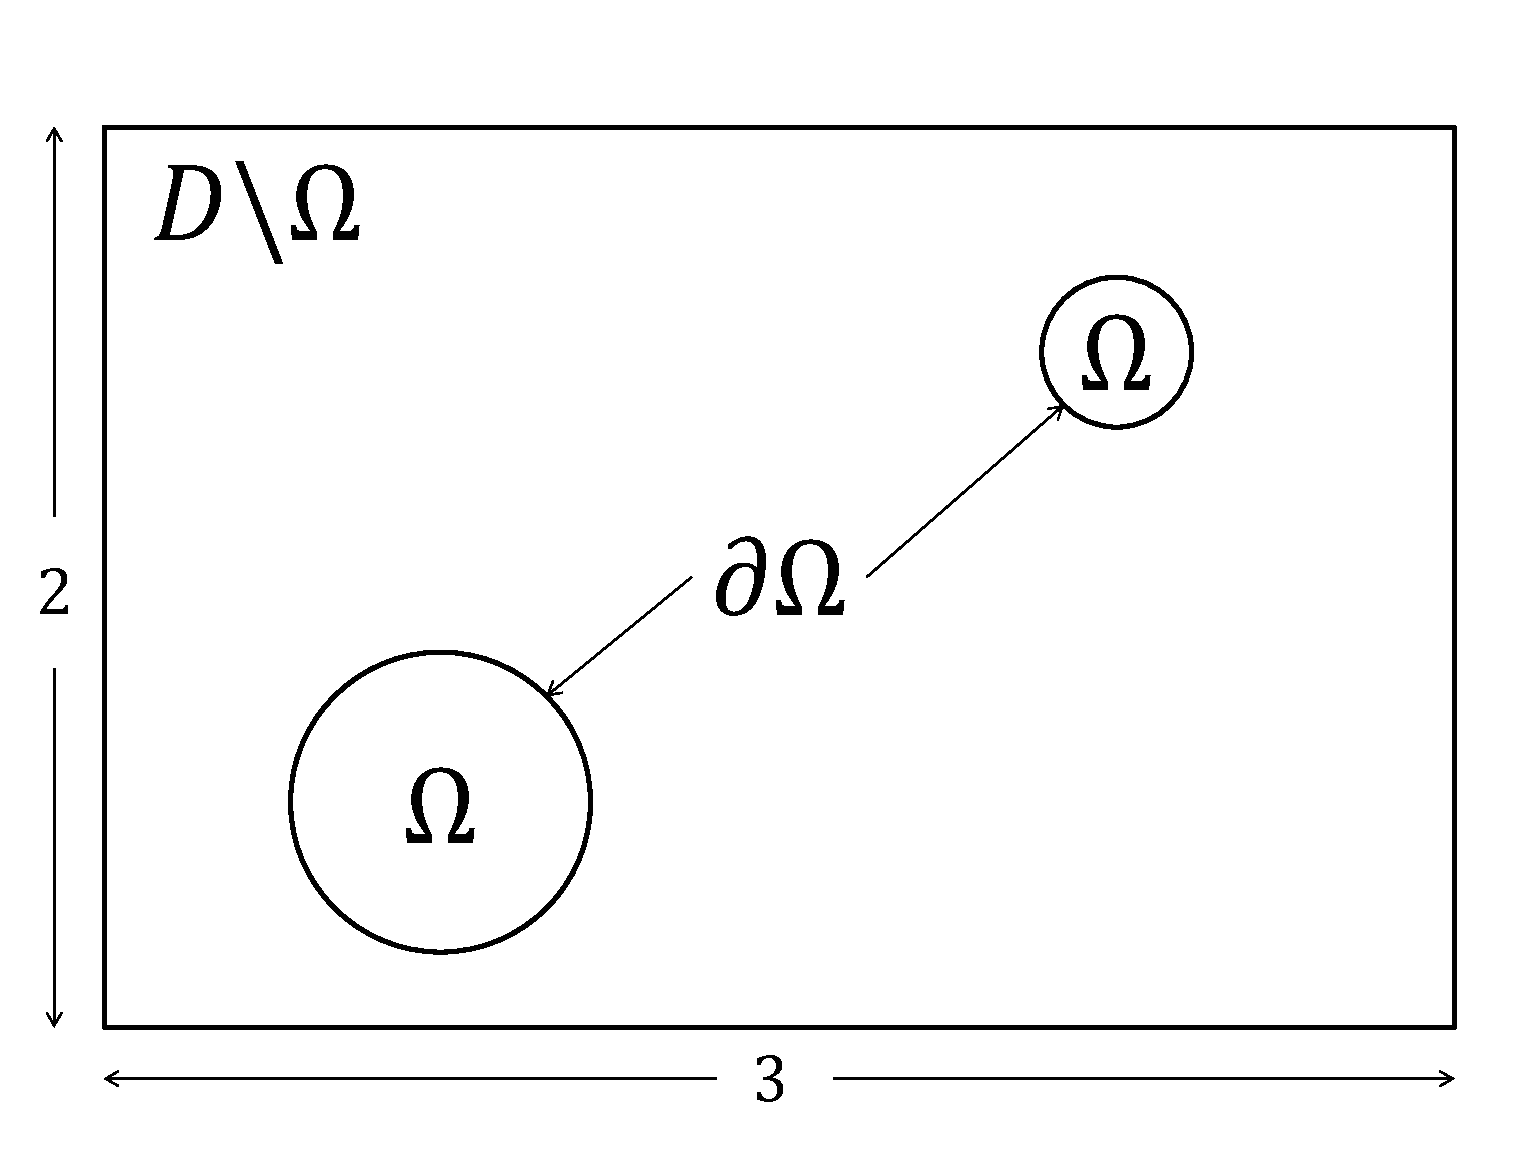
\includegraphics[width=\linewidth]{level_set_circles_1.eps}
		} &
		\subfloat[]{
			\label{fig:level_set_circle_func_025}
			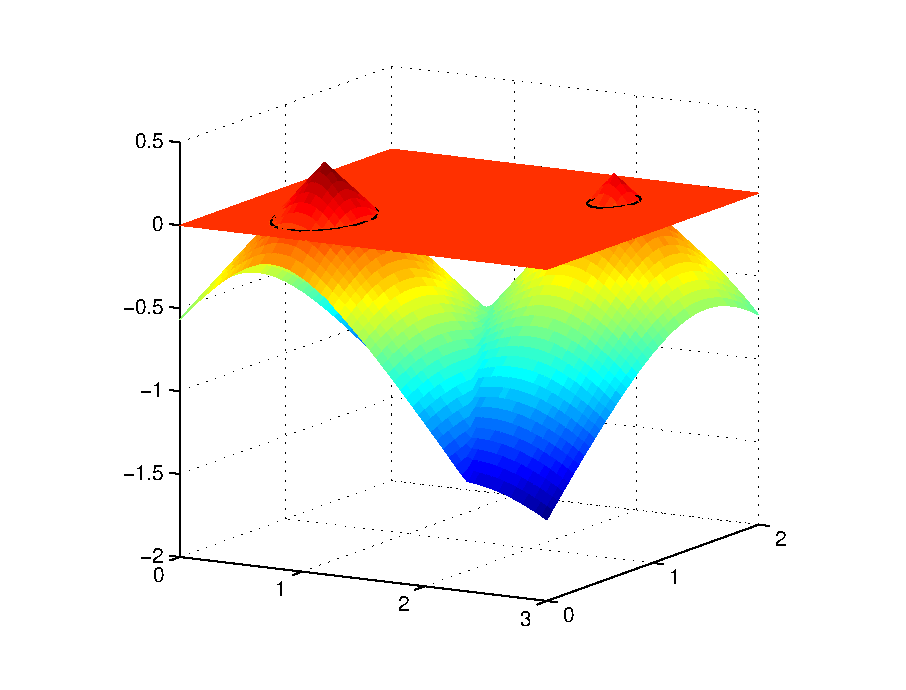
\includegraphics[width=\linewidth]{level_set_function_circles_1.eps}
		} \\
		\subfloat[]{
			\label{fig:level_set_circle_domain_050}
			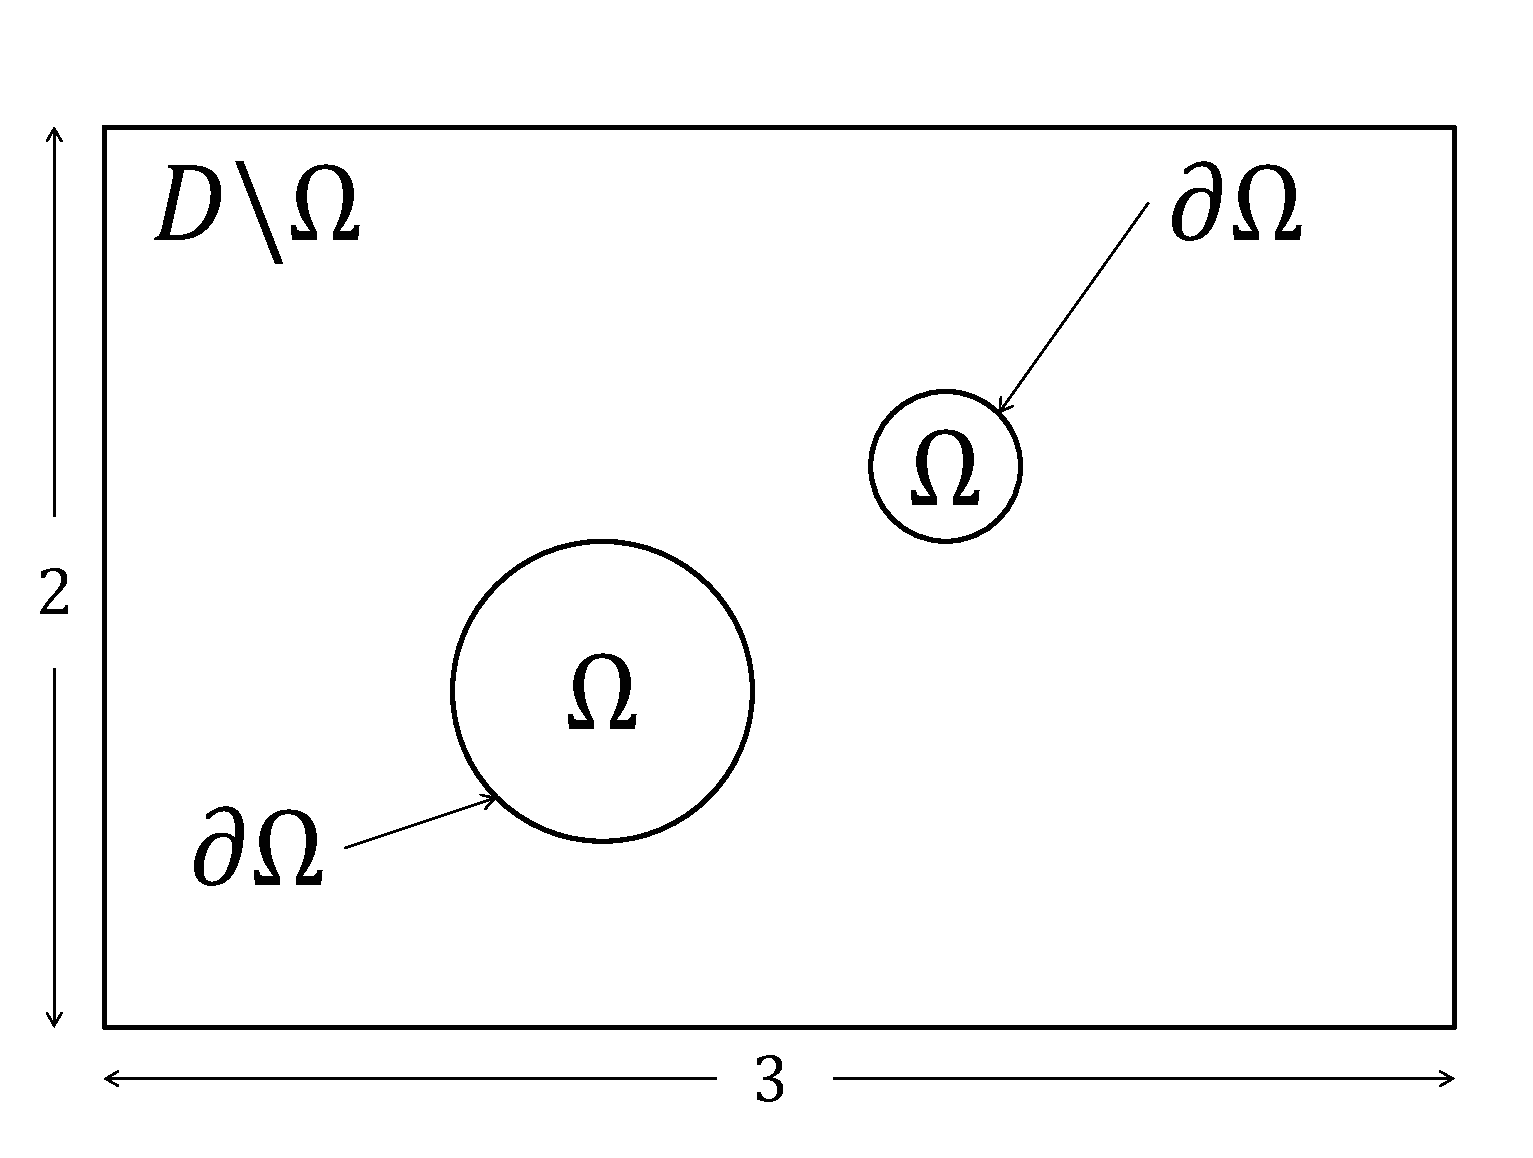
\includegraphics[width=\linewidth]{level_set_circles_2.eps}
		} &
		\subfloat[]{
			\label{fig:level_set_circle_func_050}
			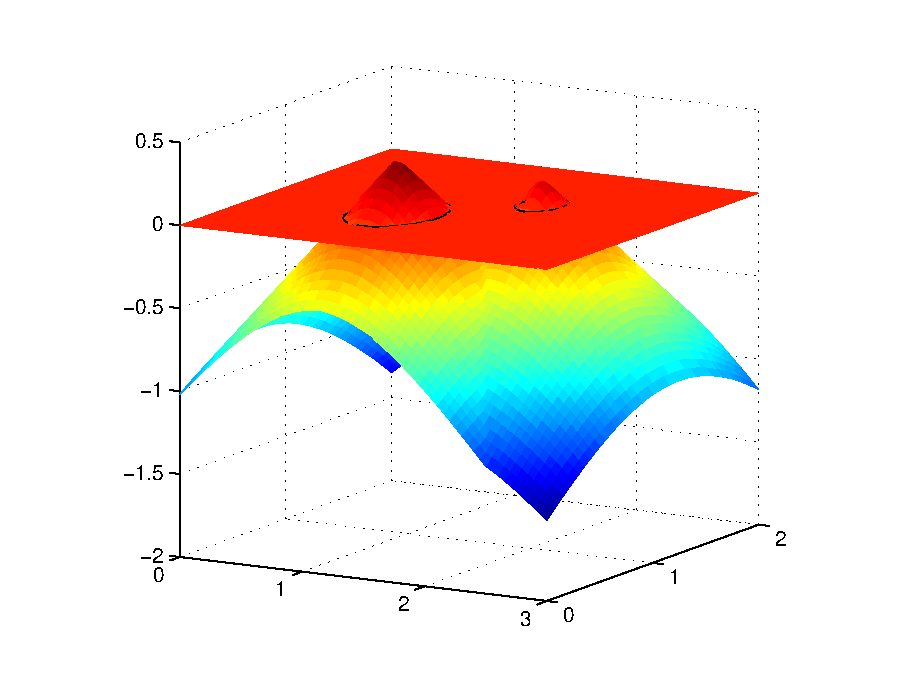
\includegraphics[width=\linewidth]{level_set_function_circles_2.eps}
		} \\
		\subfloat[]{
			\label{fig:level_set_circle_domain_075}
			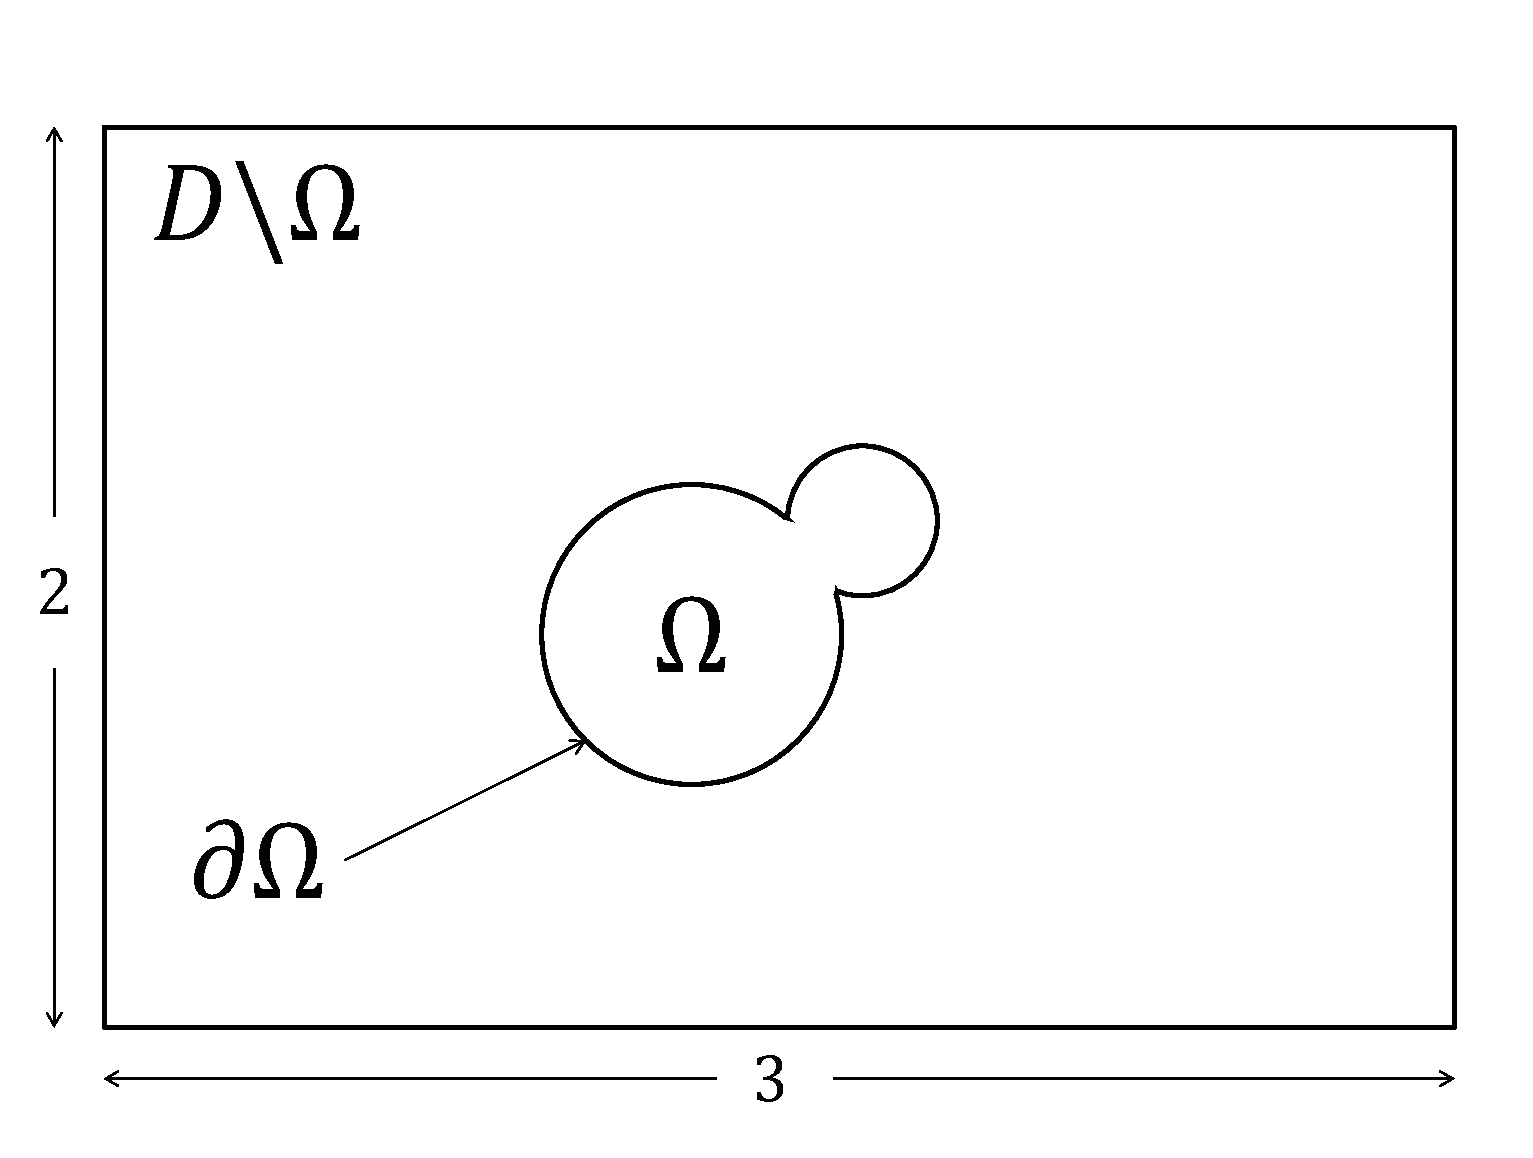
\includegraphics[width=\linewidth]{level_set_circles_3.eps}
		} &
		\subfloat[]{
			\label{fig:level_set_circle_func_075}
			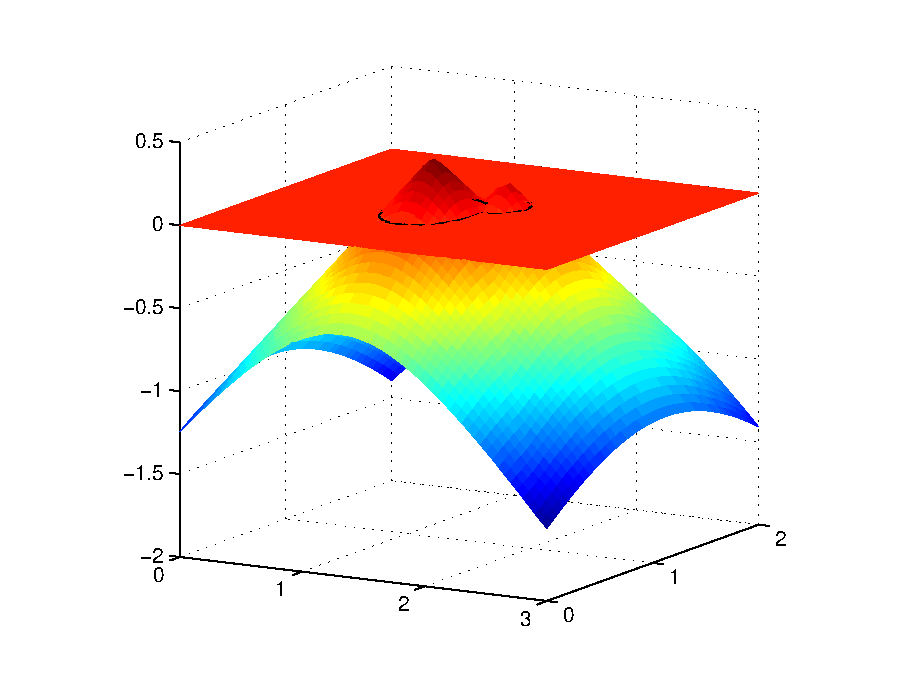
\includegraphics[width=\linewidth]{level_set_function_circles_3.eps}
		} \\
	\end{tabularx}
	\caption{Level set description of two circular inclusions with radii $0.667$ and $0.333$, respectively, moving towards each other. Level set functions can be used to describe complex topologies in a fixed mesh.}
	\label{fig:level_set_description}
\end{figure}

Multiple level set functions can be used to model more than two phase regions \ref{eq:level_set_regions}. As with the level set method itself, the use of multiple level set functions originated in image processing \citep{VC:02}. This so-called ``color'' level set method requires $m$ level set functions to model $n = 2^m$ different phase regions. For a reference on the method, the reader is referred to \citep{WW:04c,WW:05}.

The material distribution in the design domain can be determined from the phase region of the level set field. Several methods exists to describe this distribution. Density based level set methods describe the phase regions by either using element-wise constant material fractions or by mapping the level set field directly to a point \citep{YYK+:15}. These techniques are denoted as Ersatz material approaches (see Figure \ref{fig:ersatz_interpolation}) \citep{WWG:03,AJ+:05}, and while they ease the computational complexity, they lead to modeling errors. In this work, we will triangulate the element cut by the zero level set isolevel, and then perform our operations on the subdomains and on the interface (see Figure \ref{fig:XFEM_interpolation}) \citep{MM:13,VM:14}. This methodology will avoid the need to approximate material properties such as in density methods.

Regularization techniques are used in a level set optimization problem to control the geometry of the design. Among these techniques are perimeter or curvature minimization \citep{MKM+:11,YIN+:10,DLK:12}. The advantage of the level set method is that we possess a crisp definition of the phase interface, and therefore can integrate over the shape boundary $\Gamma_{\phi=0}$. These techniques will be studied in Section \ref{sec:topology_optimization_approaches_for_the_curvature_minimization_of_level_set_isocontours}.

% -----------------------------------------------------------------------------
% Topology optimization with the level set method

\subsection{Topology optimization with the level set method}

The topology of the level set field is modified by update schemes that use the sensitivities of the design variables. Several approaches exist, such as the Hamilton-Jacobi equation \citep{YNY+:10}. This work will focus on a mathematical programming approach, where the nodal values of the discrete level set field are defined as functions of the optimization design variables. Like in the filtering method of density approaches, we will define a linear filter
%
\begin{equation}
	\label{eq:smoothing_filter_XFEM}
	\phi\left(\mathbf{s}\right)=\frac{\sum_{i=1}^{N}w_{i}s_{i}}{\sum_{i=1}^{N}w_{i}}
\end{equation}

with

\begin{equation}
	\label{eq:weight_XFEM}
	w_{i}=\max \left( 0, r_{\phi} - \Vert \mathbf{x}_i - \mathbf{x} \Vert \right)
\end{equation}
%
where $\phi\left(\mathbf{s}\right)$ is the level set function at a point $\mathbf{x}$, $\mathbf{x}_{i}$ is the location of the node at which the design variable $i$ is defined, $w_{i}$ is the factor of point $\mathbf{x}$ with respect to the design variable $i$, $r_{\phi}$ is the filter radius, and $N$ is the number of nodes in the design domain. However, unlike the filter in the density approaches, this filter cannot control the minimum feature size, as discussed in Section \ref{sec:feature-size-control}.

The reader is referred to \citep{DML+:13,GP:13} for a more detailed overview of the level set method and topology optimization approaches.

% -----------------------------------------------------------------------------
% Extended finite element method

\section{Extended finite element method}
\label{sec:intro_xfem}

The extended finite element method (XFEM) is an immersed boundary technique that works on fixed meshes. The XFEM was built upon the concept of partition of unity developed by \citep{NME:NME86}, and it was originally used to model crack propagation \citep{BB:99}. Due to its ability to approximate discontinuous solutions, the method has been applied in a variety of discontinuous partial differential equations, such as multimaterial structural mechanics \citep{WW:04c,VM:14}, fluid-structure interaction \citep{GW:08}, and multi-phase flows \citep{CB:03}. The method has also been applied to shape optimization by \citep{DMJ+:06,MMF+:05,MD:07}, and to topology optimization by \citep{HMM:13,LWW:12,WWX:10,MKM+:11,MM:14,VM:14}.

The XFEM decomposes the cut elements into subdomains and interfaces that it uses to integrate the weak form of the governing equations. Figure \ref{fig:triangulation_2D} illustrates this by showing the possible decompositions of a two dimensional finite element based on its nodal level set values.
%
\begin{figure}
	\centering
	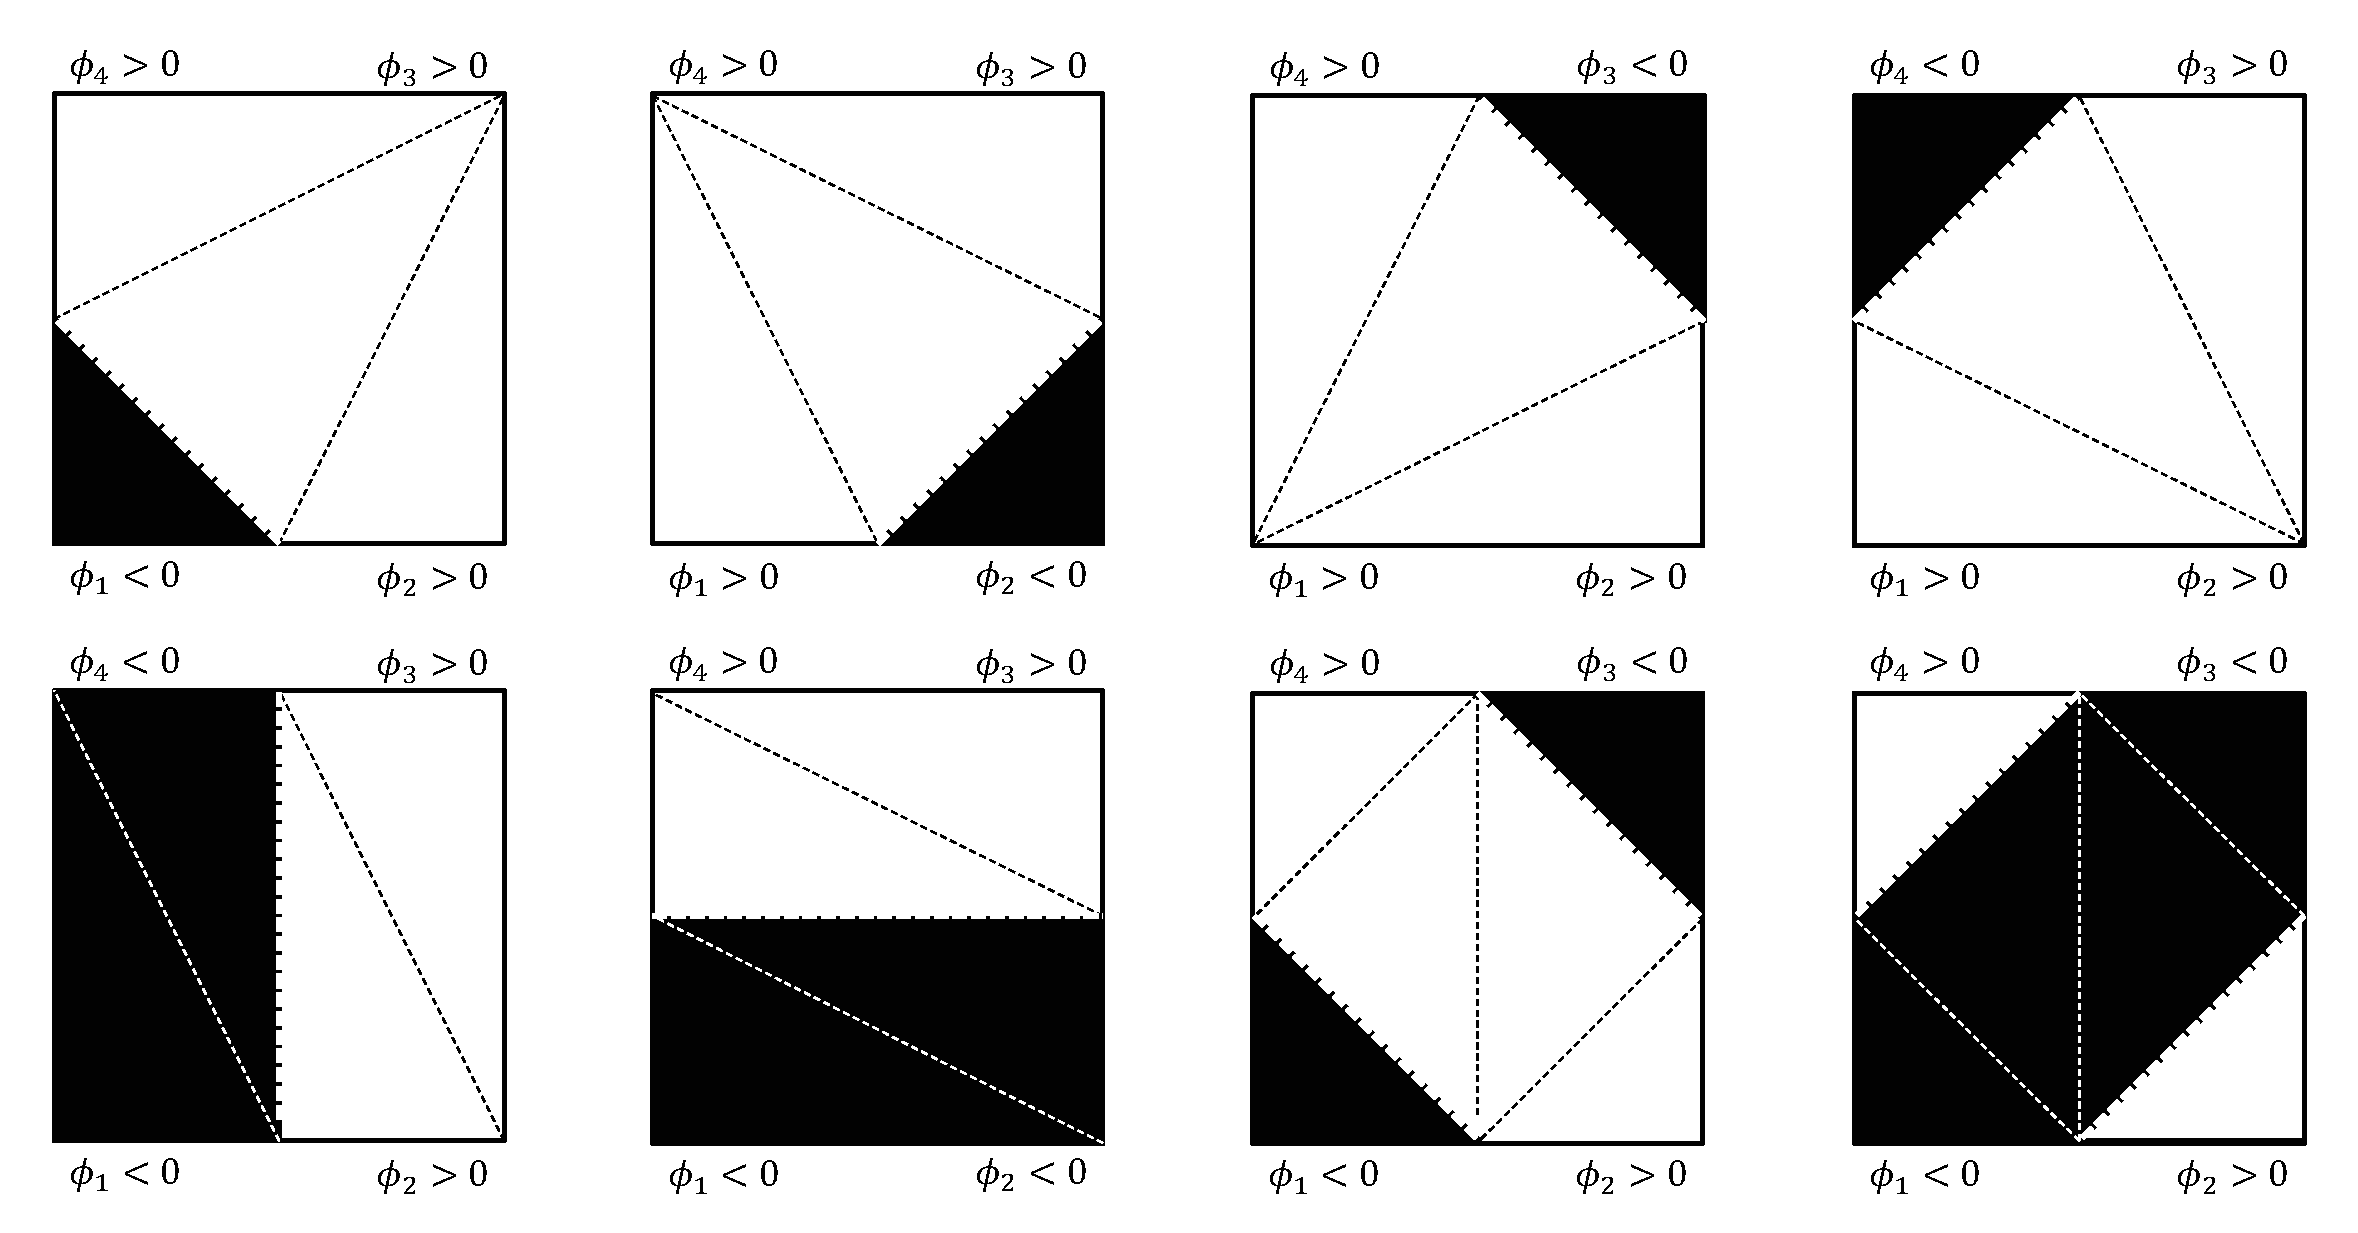
\includegraphics[width=\linewidth]{intersections_2D.eps}
	\caption{A two dimensional finite element has eight possible decompositions based on the nodal level set values.}
	\label{fig:triangulation_2D}
\end{figure}

The XFEM can model discontinuities in the solution field by augmenting the standard finite element function space with additional degrees-of-freedom, denoted ``enriched degrees-of-freedom''. To illustrate this with a quick example, consider an XFEM model that consists of a two dimensional mesh with four linear elements. The level-set distribution in Figure \ref{fig:intro_structural_model} leads to the intersection pattern shown in Figure \ref{fig:intro_physical_model}. The nodes on the left are clamped, and the right edge is subject to a constant pressure load. The node at the center of the mesh in Figure \ref{fig:intro_physical_model} will use different degrees-of-freedom to interpolate the different subdomains, and avoid artificially coupling the disconnected phase regions.
%
\begin{figure}
	\centering
	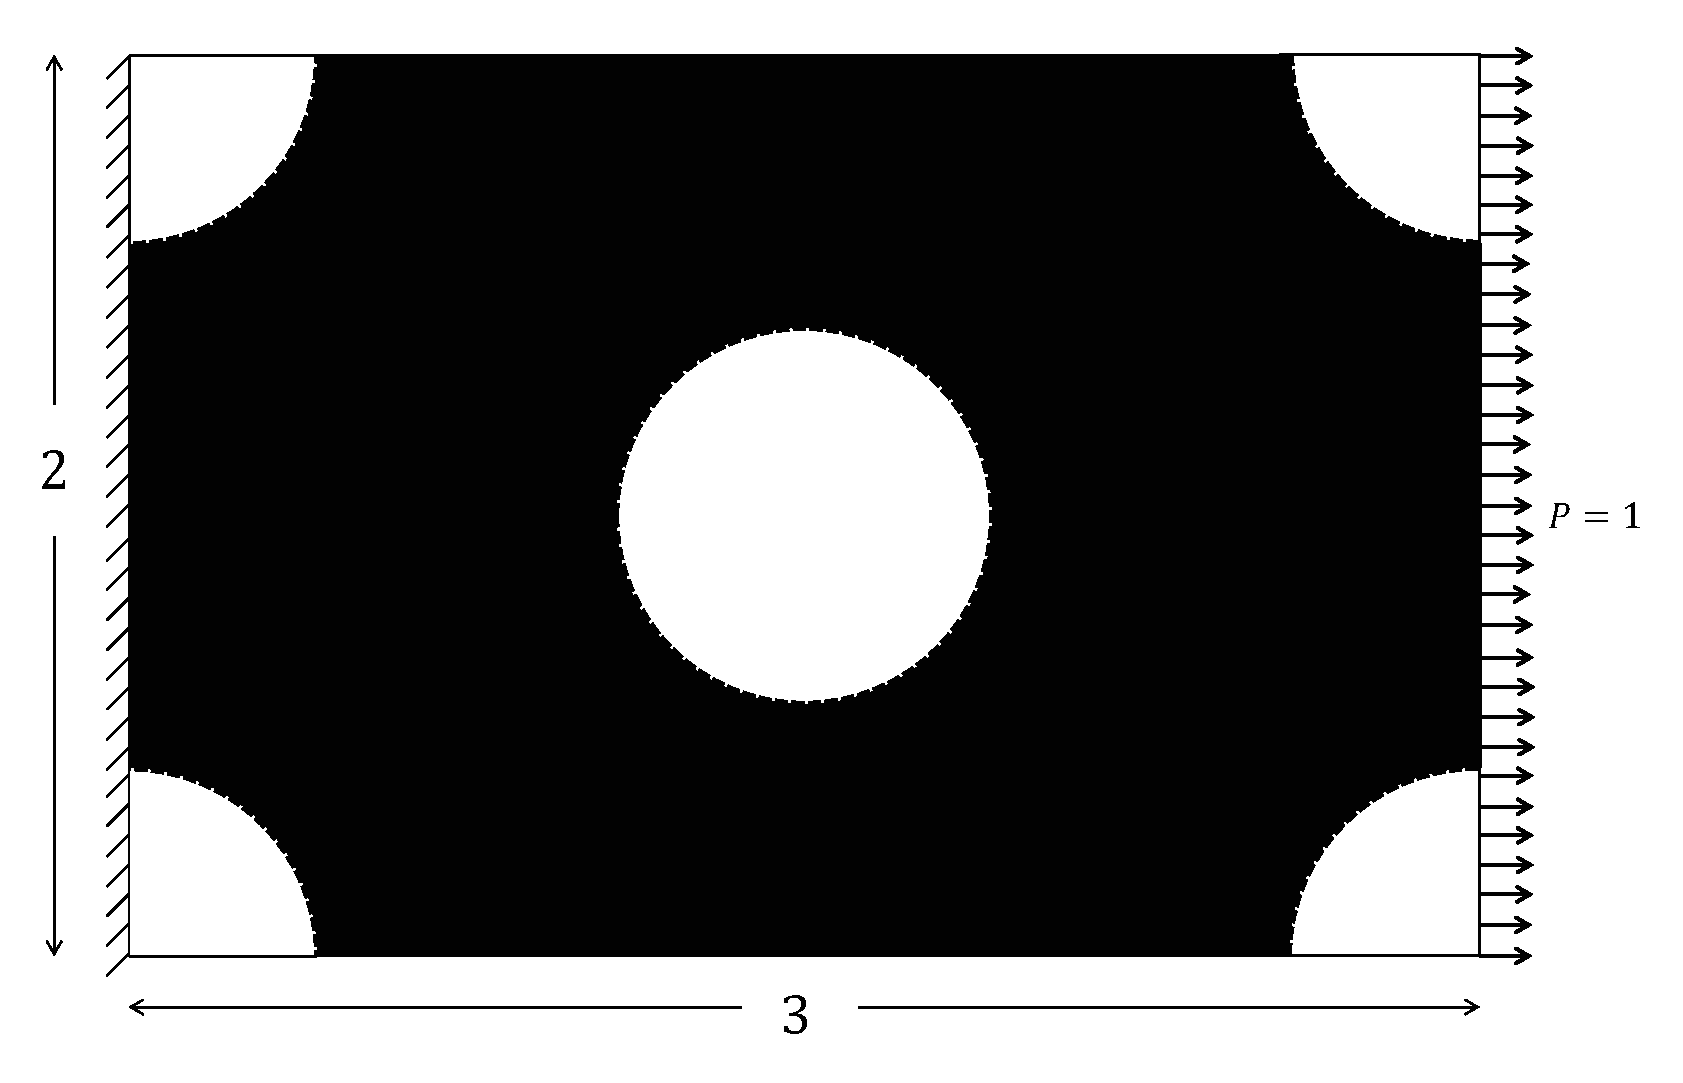
\includegraphics[width=0.75\linewidth]{structural_model.eps}
	\caption[Structural problem setup.]{Structural problem setup. The domain contains multiple level set inclusions.}
	\label{fig:intro_structural_model}
\end{figure}
%
\begin{figure}
	\centering
	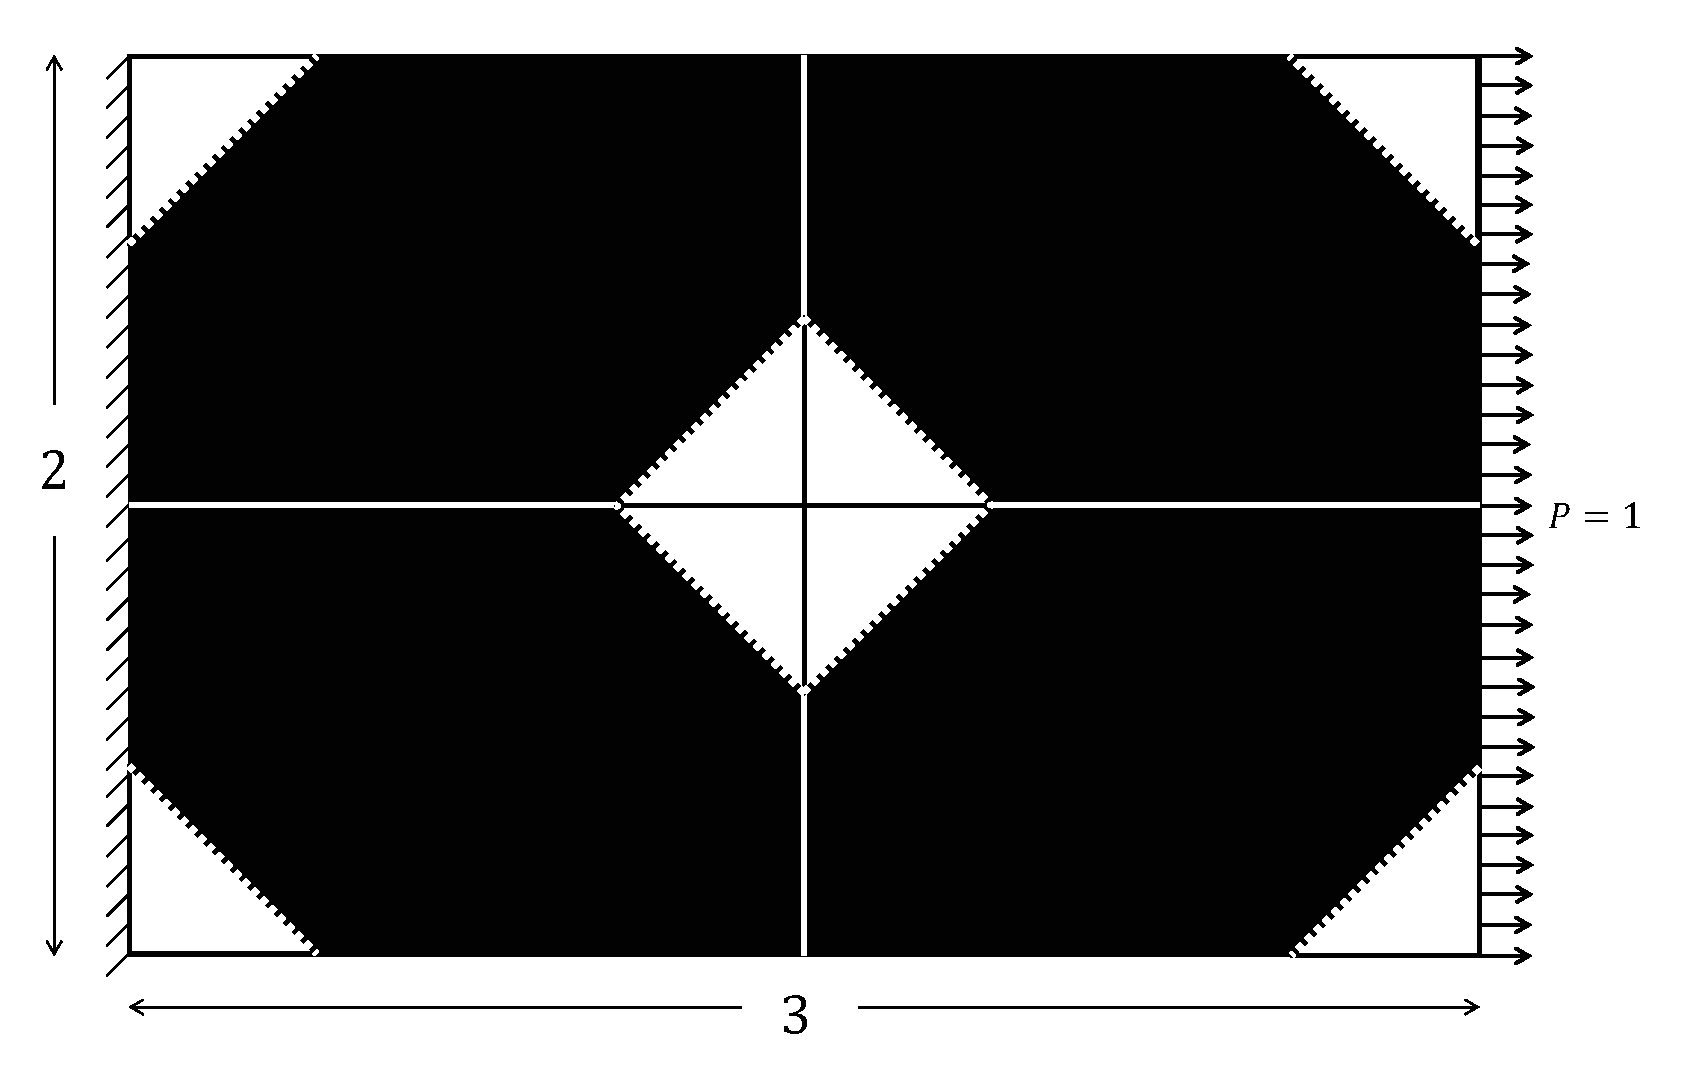
\includegraphics[width=0.75\linewidth]{physical_model.eps}
	\caption[XFEM implementation example physical model]{4-element 2D mesh. Black areas: material phase 1, negative level-set value at the nodes; white areas: material phase 2, positive level-set value.}
	\label{fig:intro_physical_model}
\end{figure}

The solution space is then interpolated using the generalized enrichment formulation of \citep{HH:04}:
%
\begin{equation}
	\mathbf{u}(\mathbf{x}) = \sum \limits^{M}_{m=1} \left( H(-\phi) \sum\limits^{n}_{i=1} \mathbf{N}_i \ \mathbf{u}_{i,m}^A
														 + H( \phi) \sum\limits^{n}_{i=1} \mathbf{N}_i \ \mathbf{u}_{i,m}^B \right)
\end{equation}

where $m$ is the enrichment level, $M$ is the maximum number of enrichment levels used for each phase, $\mathbf{N}$ are the shape functions, $\mathbf{u}^l_{i,m}$ is the vector of degrees-of-freedom values at node $i$ for phase $l=[A,B]$, $\phi$ is the level set value evaluated at $\mathbf{x}$, and $H$ denotes the Heaviside function. This is illustrated in Figure \ref{fig:intro_enrichment_model} for the structural problem of Figure \ref{fig:intro_structural_model}.
%
\begin{figure}[htbp]
	\centering
	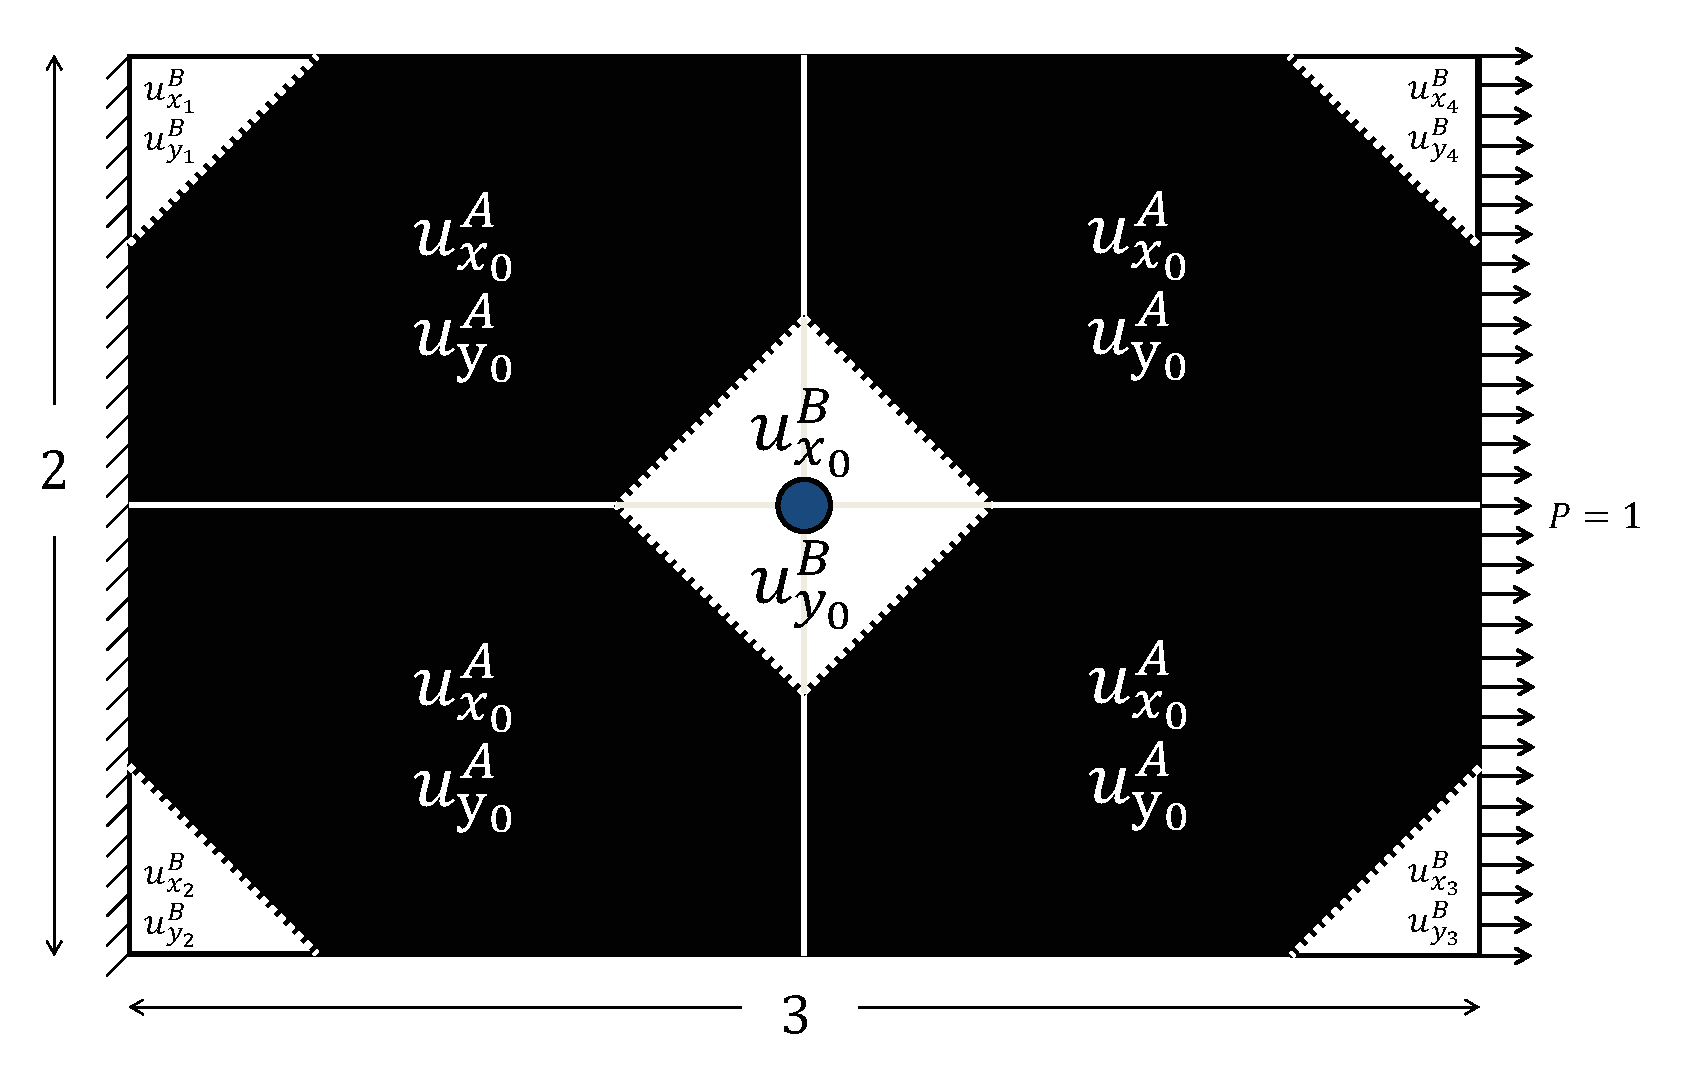
\includegraphics[width=0.9\linewidth]{enrichment_model.eps}
	\caption{The center node, denoted by the color blue, uses different degrees-of-freedom to describe the disconnected phase regions. The subscripts denote the $m$ enrichment level. The maximum number of enrichment levels used for each phase is $M=5$. A value of 0 denotes the original finite element degrees-of-freedom, while other numbers indicate additional ``enriched degrees-of-freedom''. }
	\label{fig:intro_enrichment_model}
\end{figure}

The Heaviside function $H$ depends on the level set function and is defined as follows:
%
\begin{equation}
	H(z) =
		\begin{cases}
			1 & z > 0 \\
			0 & z \le 0
		\end{cases}
\end{equation}

The Heaviside functions ``turns on/off'' the standard finite element interpolations in the particular phases. The approximation allows for discontinuities of the states $\mathbf{u}$ along the phase boundaries. Therefore, the continuity of the solution at the interface between different phase regions must be enforced. Several techniques are available in the literature, such as stabilized Lagrange multipliers (Section \ref{sec:density_and_level_set_XFEM_schemes_for_topology_optimization_of_3D_structures}) \citep{BH:10}, and the Nitsche method (Section \ref{sec:level_set_XFEM_topology_optimization_of_3D_navier_stokes_and_scalar_transport_problems}) \citep{BH:12}. More recent development include the face-oriented ghost penalty (Section \ref{sec:level_set_XFEM_topology_optimization_of_3D_navier_stokes_and_scalar_transport_problems}) by \citep{SW:14,SRG+:14,BH:12}, which aims at smoothing the gradients of the solution between cut elements. All three formulations will be studied and applied to topology optimization in this work.

For more details, refer to Sections \ref{sec:a_complete_methodology_for_the_implementation_of_XFEM_inclusive_models}, \ref{sec:discretization}, and \ref{sec:computational-considerations}. For a review of the XFEM, the user is referred to \citep{FB:10}.

% -----------------------------------------------------------------------------
% Available software

% \section{Available software}

% For the numerical modeling and simulation, we will use our in-house code, the Finite Element Multidisciplinary Optimization Code (FEMDOC). The linear algebra package is provided by Trilinos \citep{Trilinos:03}.

% -----------------------------------------------------------------------------
%
%* What is your work about?
%
%- Topology optimization approach.
%- Using the Level Set Method.
%- eXtended Finite Element Method.
%- LSM describes the geometry of the design.
%- XFEM is used to solve the PDE and measure the performance.
%- Apply methodology for complex work.
%
%* Who should care about your work?
%
%- Topology optimization community. 
%- Alternate method to homogenization methods.
%- Design engineers.
%- Surface mesh ready for three dimensional printing.
%
%* What are the goals of your thesis?
%
%- Develop robust topology optimization approach using the LSM and the XFEM methods.
%- Compare pros and cons against homogenization methods.
%- Apply methodology to real-world problem, such as ALD.
%
%* What is your overarching approach? How will you know you have accomplished your goals?
%
%- Develop methodology for triangulation, enrichment of 3D geometries (methodology section).
%- Test framework with structural problems in three dimensions (structural section).
%- Compare results with SIMP (structural section).
%- Expand to incompressible Navier-Stokes and Stokes flows, and scalar transport (fluids section).
%- Study convergence with respect to the enforcement of boundary conditions to ensure stability and coercivity.
%- Study convergence with respect to intersection configuration.
%- Study shape control and regularization techniques (curvature section).
%- Three dimensional printing (structural, fluids, curvature sections).
%- Apply methodology to ALD problem (ALD section).
%
%* Why should they care about your work?
%
%- Methodology accommodates different physics.
%- Accommodate structural, Navier-Stokes, scalar transport physics.
%- Three dimensional problems.
%- For topology optimization, it is relevant because it provides an alternate method besides homogenization methods.
%- Advantages over SIMP.
%- Explicit description of boundary for correct application of boundary conditions.
%- Regularization techniques allow shape control of the interface.
%- Prevents spurious diffusion, etc.
%- Coarser mesh leads to faster computations.
%
%* Does it enable us to solve new optimization problems or just live with coarser mesh?
%
%- Solve topology optimization problems where physics at interface is crucial.
%- ALD requires measuring temperature distribution correctly. Spurious diffusion does not help the problem.
%- Coarse mesh is good enough to describe physics at the interface.
%- In 3D, efficiency is crucial.
%
%* How is thesis proposal structured?
%
%- What sections present?
%- Mention sections are drafts of papers.
\section{Implementation}
\label{implementation}

%----------------------------------------------------------------------------------------
% Summary

\subsection{Summary}

This document outlines the procedure for building an XFEM model for a given distribution of the level-set function. The XFEM model consists of:
\begin{itemize}
\item Intersection points along elemental edges.
\item XFEM elements sub-divided into cells for integrating the weak form of the governing equations within the individual sub-domains belonging to a particular material phase.
\item Enrichment tables that define the nodal enriched degrees of freedom used to interpolate the solution within a cell.
\item Parallel implementation of building XFEM model.
\end{itemize}

%----------------------------------------------------------------------------------------
% Glossary

\subsection{Glossary}

\noindent
\textbf{computational mesh} -- standard FE mesh that defines the nodal degrees of freedom. \\
\textbf{model} -- physical entity, contains information about the XFEM elements and the level-set functions. \\
\textbf{main phase (phase)} -- phase indicating a particular material phase. \\
\textbf{sub-phase} -- the domain of a main phase can be decomposed into multiple sub-phases. \\
\textbf{intersection point} -- intersection created by the zero level-set curve cutting through an edge. \\
\textbf{point} -- geometrical entity with information about coordinates, connected cells and edges. \\
\textbf{cell} -- geometrical entity, a collection of points, owns a list of edges too. \\
\textbf{edge} -- geometrical entity with information about the points on its ends and its connected cells. \\
\textbf{Delaunay triangulation} -- triangulation of our elements using their corner nodes and intersection points. \\
\textbf{pseudo-element} -- cells created by the triangulation of the regular element. \\
\textbf{nodal cluster} -- set of elements (and their nodes) connected to a node
consistency nodes	nodes shared by multiple elements within nodal cluster. \\

%----------------------------------------------------------------------------------------
% Procedure

\subsection{Procedure overview}

The main steps are:
\begin{enumerate}
\item Build point-to-cells connectivity list (list of cells connected to a point) by looping over all cells; needs to be built only once.
\item Build edge table in mesh (list of the cell edges that stores connectivity to points and cells) by looping over all cells; needs to be built only once.
\item Build table of nodes belonging to a nodal cluster (first-order neighbors of a node; defined as all nodes belonging to elements connected to a node) by looping over all elements for a node using point-to-cell table; needs to be built only once.
\item Build edge intersection points by looping over all edges; points are stored in mesh; however, the coordinates of the intersections are copied to the XFEM element; needs to be built for each instance of a level-set distribution.
\item Delaunay triangulation of each cell based on edge intersection; needs to be built for each instance of a level-set distribution.
\item Build table of phases and sub-phases for each triangle/tetrahedron (pseudo-cells) for each triangulated element; needs to be performed for each instance of level set distribution.
\item Build enrichment table that defines which nodal degrees of freedom are used to interpolate a field within a pseudo-element.
\item Determine which degrees of freedom are used in the model.
\end{enumerate}

%\begin{figure}[htbp]
%	\centering
%	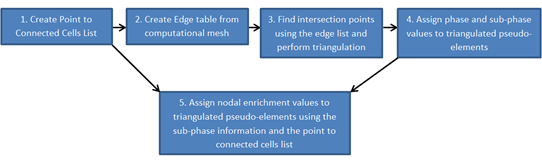
\includegraphics[scale=1]{./img/procedure_overview.png}
%	\caption[XFEM Overall Procedure]{The diagram shows the overall procedure required to implement the XFEM model.}
%	\label{fig:Overall-Procedure}
%\end{figure}

% -----------------------------------------------------------------------------
% XFEM implementation algorithms

\subsection{Implementation algorithms}
\label{sec:implementation}

Consider the following XFEM model which consists of a 4-element mesh in 2D; the nodes on the left are clamped and the right edge is subject to a constant pressure load. The level-set distribution in Figure \ref{fig:structural_model} leads to the intersection pattern shown in Figure \ref{fig:physical_model}. The mesh in Figure \ref{fig:discrete_model} shows the indices of the nodes and the cells.

\begin{figure}[htbp]
	\centering
	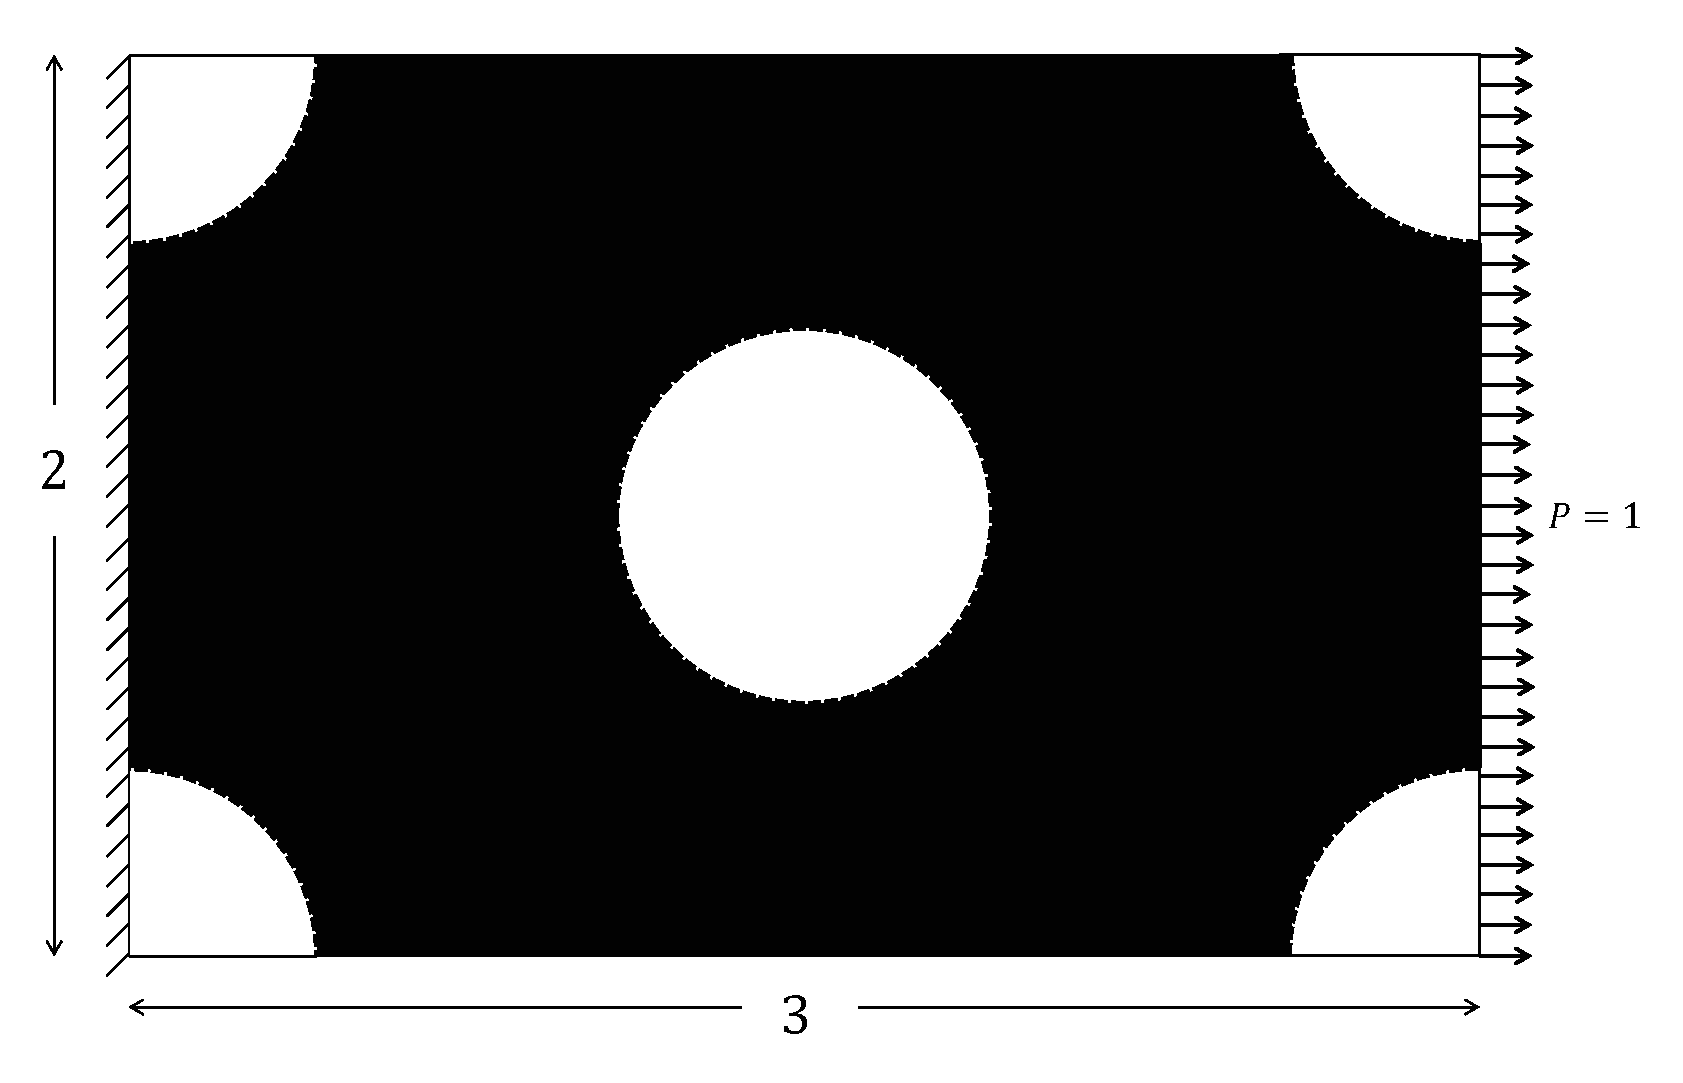
\includegraphics[width=0.75\linewidth]{structural_model.eps}
	\caption[Structural problem setup.]{Structural problem setup. The domain contains multiple level set inclusions.}
	\label{fig:structural_model}
\end{figure}

\begin{figure}[htbp]
	\centering
	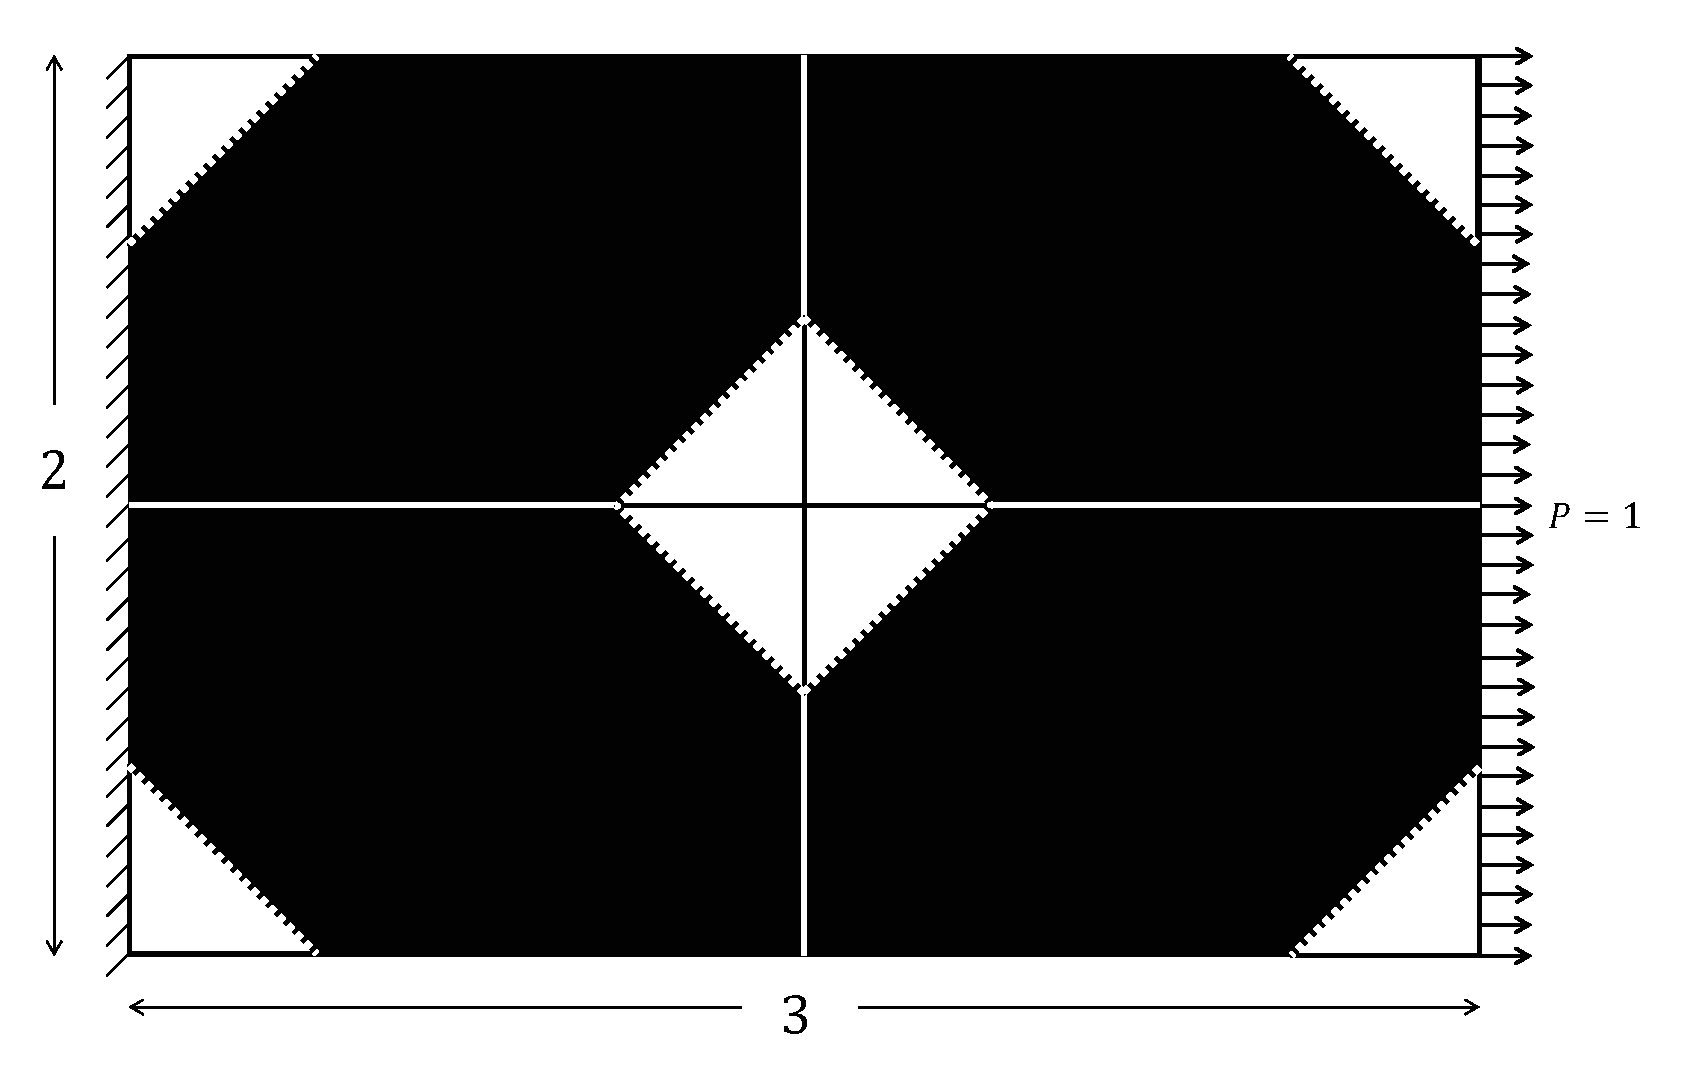
\includegraphics[width=0.75\linewidth]{physical_model.eps}
	\caption[XFEM implementation example physical model]{4-element 2D mesh. Black areas: material phase 1, negative level-set value at the nodes; white areas: material phase 2, positive level-set value.}
	\label{fig:physical_model}
\end{figure}

\begin{figure}[htbp]
	\centering
	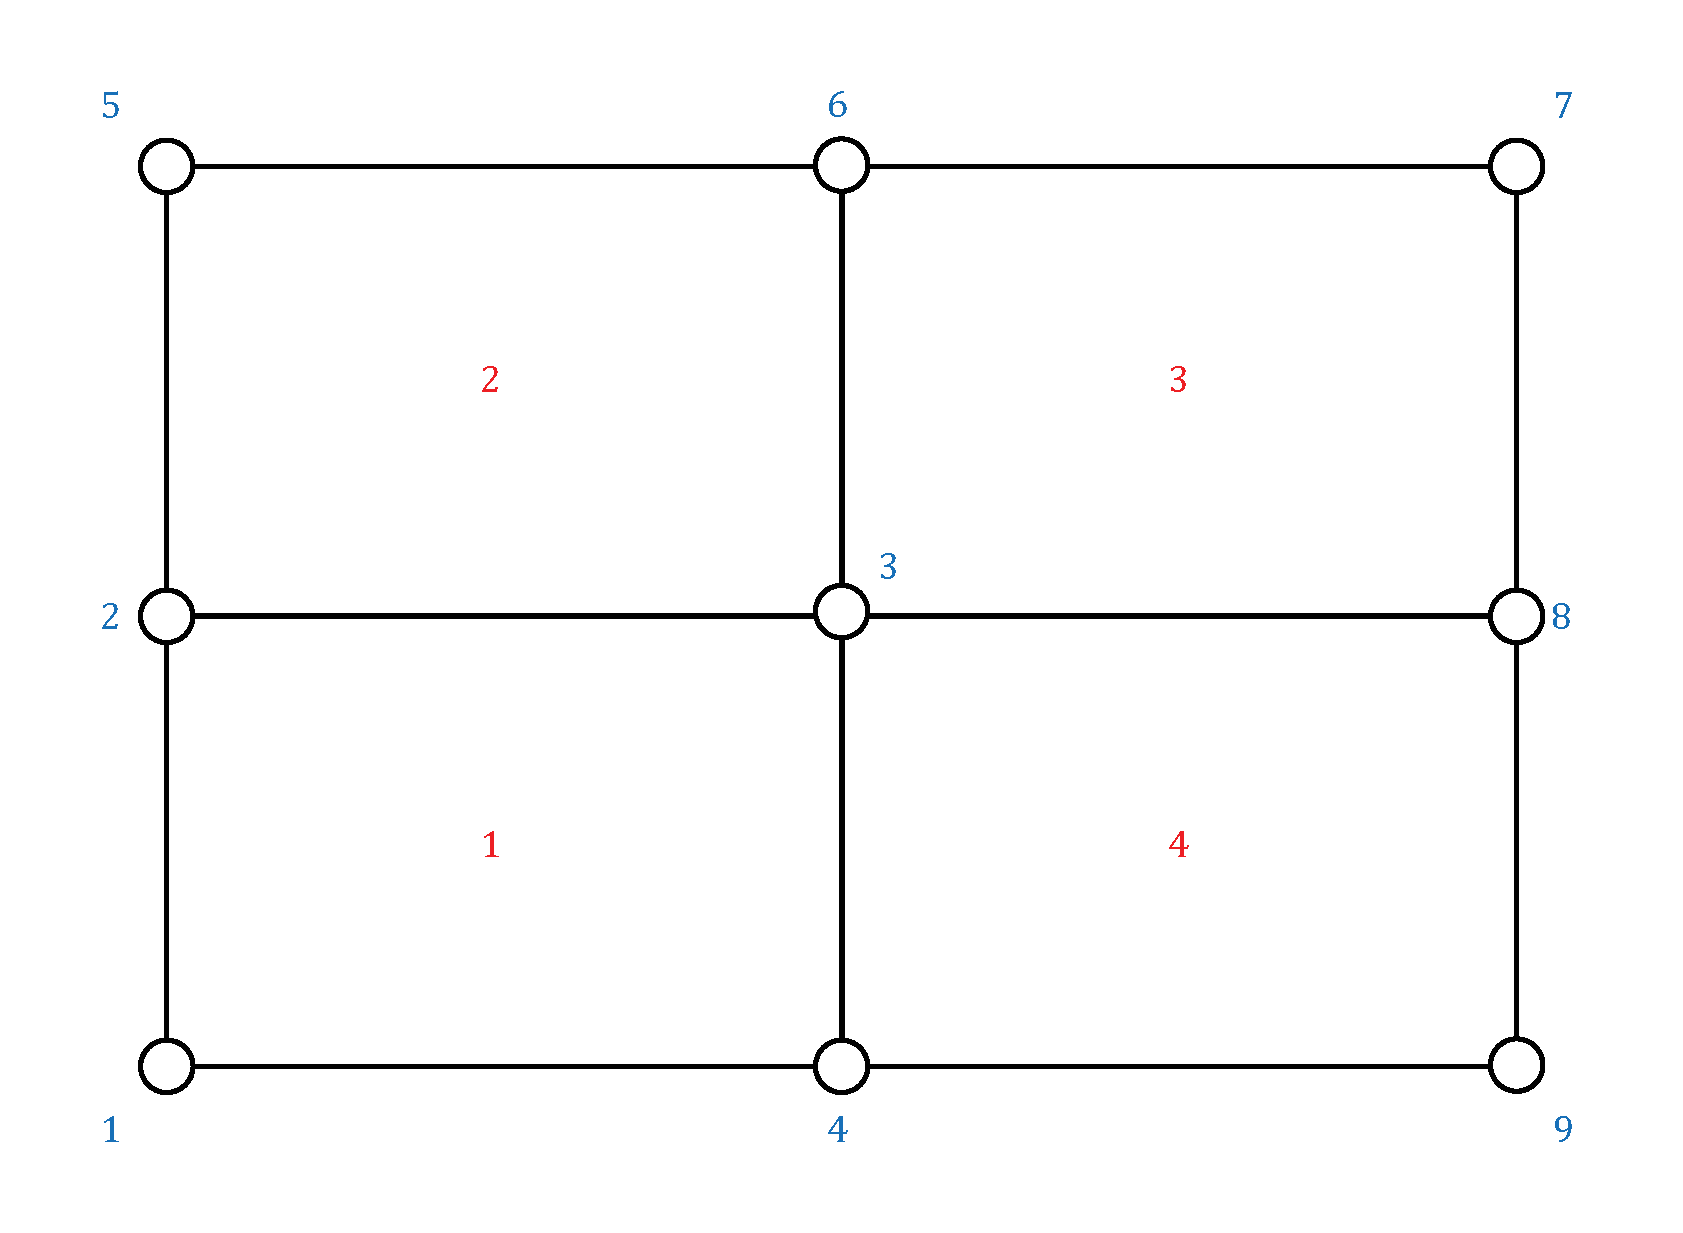
\includegraphics[width=0.75\linewidth]{discrete_model.eps}
	\caption[XFEM implementation example discrete model]{4-element 2D mesh. Red numbers represent the global element identifiers, blue numbers represent the global node identifiers.}
	\label{fig:discrete_model}
\end{figure}

% -----------------------------------------------------------------------------

\subsubsection{Point-to-cells connectivity table}

To build a point-to-cell table for each point in our computational mesh we loop over all base cells in the computational mesh (base cells are all cells that are not side-set cells). For each base cell we loop over all points and store the current cell index with point index. This leads to the point-to-cell connectivity table (see Table \ref{tab:point-to-cell-connectivity-table}):

\begin{table}[htbp]
	\centering
		\begin{tabular}{| l | l | l |}
		\hline
		Point Id & Number of cells connected & Cell Ids \\ \hline
		1 & 1 & 1		\\ \hline
		2 & 2 & 1,2		\\ \hline
		3 & 4 & 1,2,3,4 \\ \hline
		4 & 2 & 1,4 	\\ \hline
		5 & 1 & 2 		\\ \hline
		6 & 2 & 2,3 	\\ \hline
		7 & 1 & 3 		\\ \hline
		8 & 2 & 3,4 	\\ \hline
		9 & 1 & 4   	\\ \hline
		\end{tabular}
	\caption[Point ID to cell IDs connectivity table]{Point ID to cell IDs connectivity table}
	\label{tab:point-to-cell-connectivity-table}
\end{table}

% -----------------------------------------------------------------------------

\subsubsection{Edge table}
\label{sec:edge-computation}
To generate an edge table in our computational mesh we initially loop over all base cells. For each cell, we determine the number of edges and loop over all edges in the cell. For each edge, we check with the current element whether the edge has been created. In case the edge does not exist yet, we store the following edge information:

\begin{itemize}
\item Ids of end point of edge.
\item Ids of cells to which element is connected.
\end{itemize}

We determine the cells which are connected to an edge via the intersection of cells connected to the end points of the edge, using the point-to-cell table. The following edge table is stored with the computational mesh. 

At this point, each global edge knows the point Ids on its ends and the cell Ids of the elements it is connected to. We can use this information to create a map that links the global edge to the local edge index per element. Each element has an internal edge order list pre-built that indicates the order in which its edges are organized. For example, a QUAD4 element will have the following internal edge order list: 0 1, 1 2, 2 3, 3 0. The element also knows the point Ids that it owns (if not directly, point Ids can be obtained through the nodes). Using these two lists, we can compute which point Ids lay in each of the element's internal edges. By matching the point Ids of the global edge to the point Ids of the internal element edges, we can make a map that tells us which internal edge in an element corresponds to a global edge. This list is stored with the edge in the same manner that cell Ids are stored. Cell Ids and internal edge numbers should have a one to one correspondence.

For example, for the 4-element cluster above we would obtain 12 global edges (see Table \ref{tab:edge-table}).

\begin{table}[htbp]
	\centering
		\begin{tabular}{| l | l | l | l |}
		\hline
		Global Edge Id & Point Ids & Cell Ids & Local Edge Num \\ \hline
		1  & 1, 4 & 1   & 0 	\\ \hline
		2  & 3, 4 & 1 4 & 1, 3 	\\ \hline
		3  & 2, 3 & 1 2 & 2, 0 	\\ \hline
		4  & 1, 2 & 1   & 3 	\\ \hline
		5  & 4, 9 & 4   & 0 	\\ \hline
		6  & 8, 9 & 4   & 1 	\\ \hline
		7  & 3, 8 & 3 4 & 0, 2 	\\ \hline
		8  & 2, 5 & 2   & 3 	\\ \hline
		9  & 5, 6 & 2   & 2 	\\ \hline
		10 & 3, 6 & 2 3 & 1, 3	\\ \hline
		11 & 6, 7 & 3   & 2 	\\ \hline
		12 & 7, 8 & 3   & 1 	\\ \hline
		\end{tabular}
	\caption[Edge to points and cells IDs connectivity table]{Edge to points IDs and cells IDs connectivity table}
	\label{tab:edge-table}
\end{table}

The table shows, for example, that the global edge 2 is defined by the point Ids 3 and 4 and is connected to cells with Ids 1 and 4. For cell id 1, it is the local edge 1 (counting from zero CCW starting at the bottom) and for cell id 4 it is local edge 3 (Figure \ref{fig:edge-discretization}).

\begin{figure}[htbp]
	\centering
	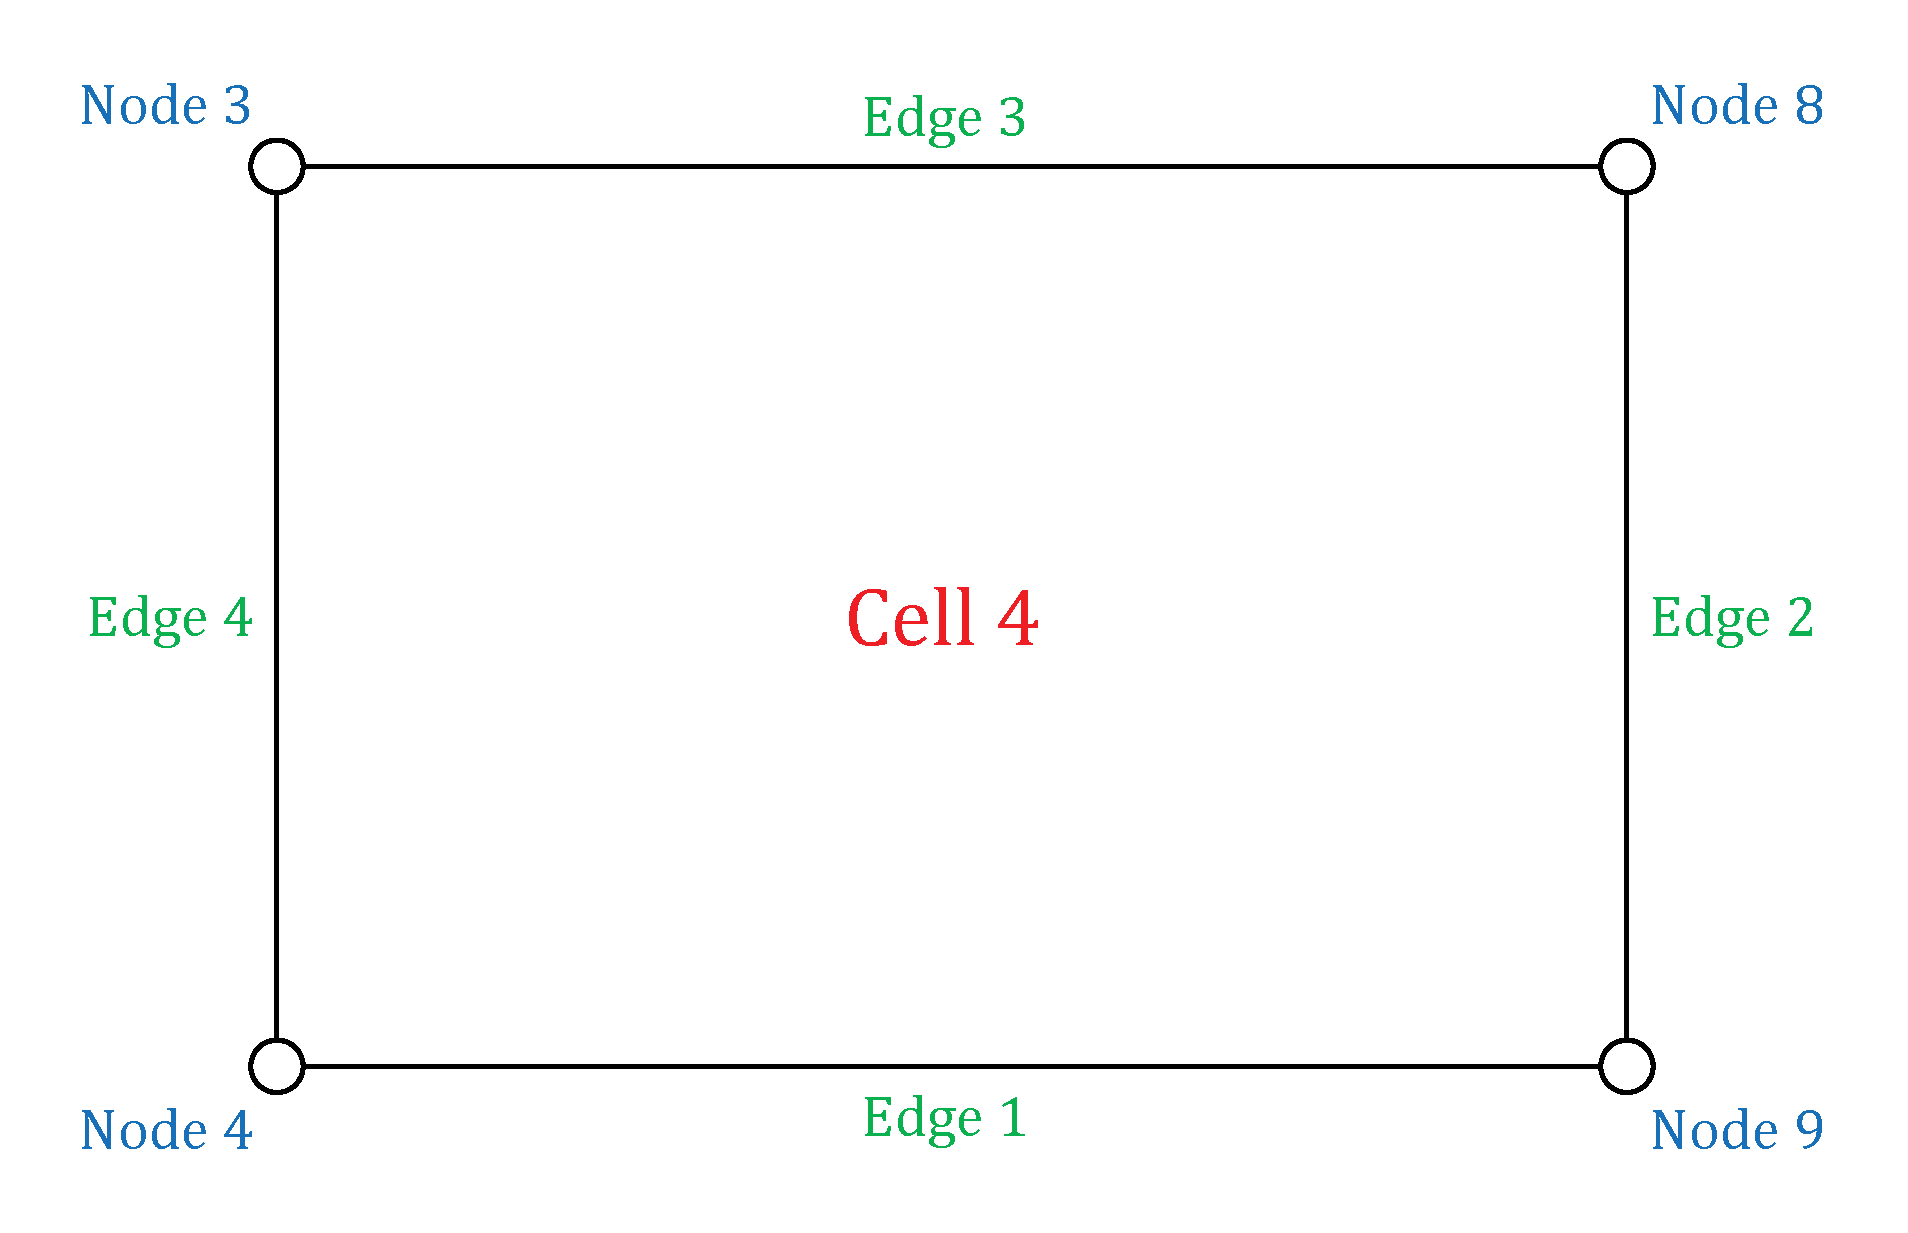
\includegraphics[width=0.7\linewidth]{edge_discretization.eps}
	\caption[Edge discretization of XFEM model example]{Edge representation in a QUAD4 element. Green edges represent the local edge index at the element.}
	\label{fig:edge-discretization}
\end{figure}

% -----------------------------------------------------------------------------

\subsubsection{Nodal clusters}

To determine the enrichment level used to interpolate fields within the XFEM elements we need to determine the first-order nodal neighbors of a node. This is the set of nodes that belong to the elements connected to a node. In addition, we need to identify the nodes that belong to two or more elements; we refer to these nodes as consistency nodes. Consistency nodes are simply the nodes in a nodal cluster (nodes of the connected elements of a main node) that are shared by more than one element in the nodal cluster. This information can be obtained by looping over the connected elements of a node, and obtaining the node list for each element. 

% -----------------------------------------------------------------------------

\subsubsection{Determine intersection points}

The intersection points are defined by the zero level-set values. We loop over all edges defined in the edge table created in Step 2 and compute the intersection points along the edge using the nodal level-set information of the edge endpoints.  The coordinates of the intersection points are then sent to all elements connected to the edge and stored in the corresponding XFEM element. (see Figure \ref{fig:intersection_point}). NOTE: Since edges only know of the cells connected to it, we use a cell-to-element map in order to be able to send this information to the XFEM elements. This is owned by the model.

\begin{figure}[htbp]
	\centering
	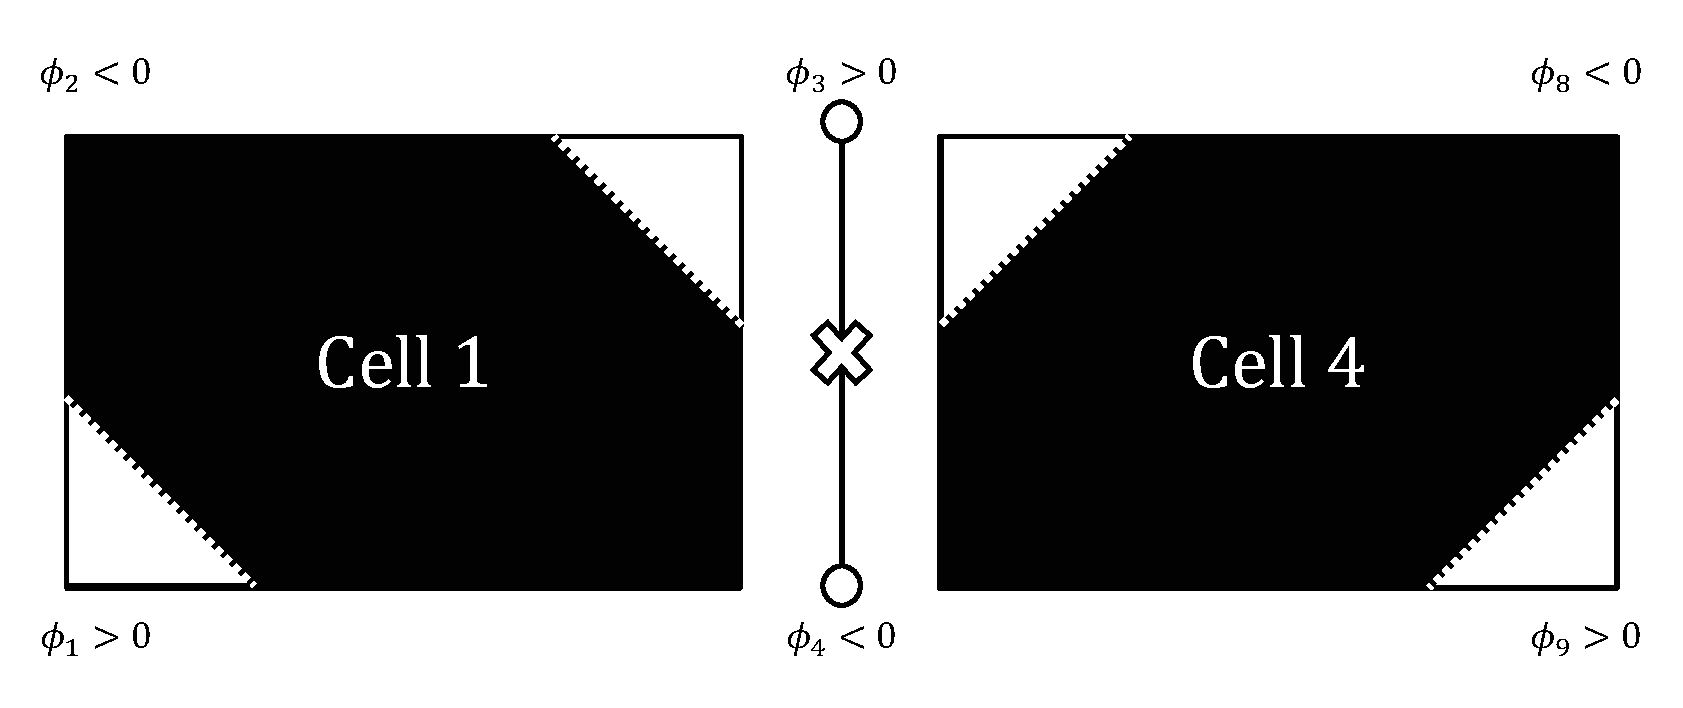
\includegraphics[width=\linewidth]{intersection_point.eps}
	\caption[Intersection point computation]{Mapping of the intersection points to the elements. An edge contains two nodes that have level set values of opposite sign. The location of the intersection point is labeled with an ``X'' in the figure. The information of the intersection point is sent to all the neighboring elements of the edge.}
	\label{fig:intersection_point}
\end{figure}

% -----------------------------------------------------------------------------

\subsubsection{Delaunay triangulation and assignment of main and sub-phases to pseudo-elements}

We loop over all elements in the model and, if intersected, we perform a Delaunay triangulation, using the corner nodes and the edge intersection points stored with the elements in Step 3. The Delaunay triangulation requires only the coordinates of the element corner and edge intersection points. The Delaunay triangulation will return a list of triangles for 2D or tetrahedrons for 3D problems. 

% -----------------------------------------------------------------------------

\subsubsection{Main phase and sub-phase}
\label{sec:main-phase-sub-phase}

We assign a main and sub-phase to each triangle/tetrahedron. The main phase is determined based on the average main-phase value of the pseudo-element.  In case the average is zero, we apply an exception rule (TBD). The sub-phase information is based on the connectivity of pseudo-elements which belong to the same main phase and is computed via a \href{http://en.wikipedia.org/wiki/Flood_fill}{flood-fill algorithm}. To this end we collect the pseudo-elements into a pseudo-mesh; each triangulated XFEM element has its own pseudo-mesh which consists of the points and the connectivity of the pseudo-elements.
The main steps (Figure \ref{fig:subphase_algorithm}) of the flood-fill algorithm used are:

\begin{itemize}
\item Build edge table for pseudo-elements of current XFEM element, analogue to Step \ref{sec:edge-computation}.
\item Loop over all elements that have not been assigned a sub-phase:
	\begin{itemize}
	\item Find unprocessed element; recursively find neighbors with same main-phase; assign lowest unassigned sub-phase to elements found in search process.
	\end{itemize}
\end{itemize}

\begin{figure}[H]
	\centering
	\begin{tabularx}{\linewidth}{XXX}
		\subfloat[Start with the first subphase value of the first main phase. Do so by selecting the first cell in the triangulation list without a value assigned.]{
			\label{fig:subphase_algorithm_1}
			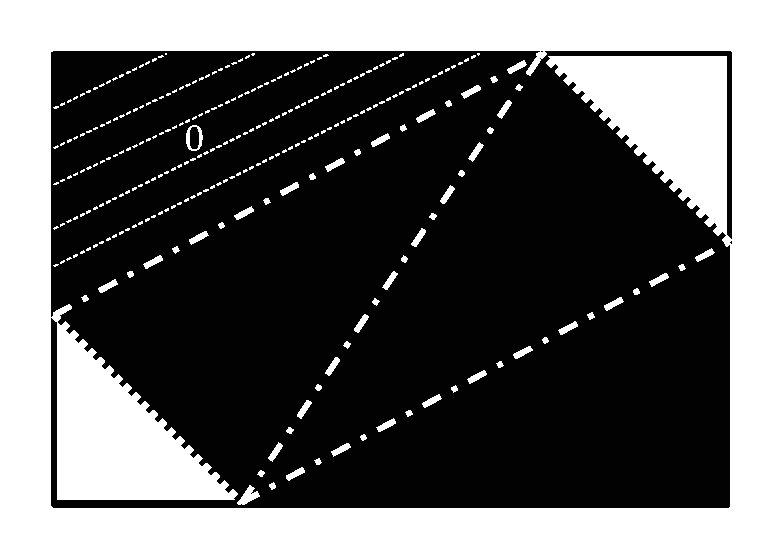
\includegraphics[width=\linewidth]{subphase_algorithm_1.eps}
		} &
		\subfloat[Look for connected cells through edges. If two cells share the same main phase and are connected, then they have the same subphase.]{
			\label{fig:subphase_algorithm_2}
			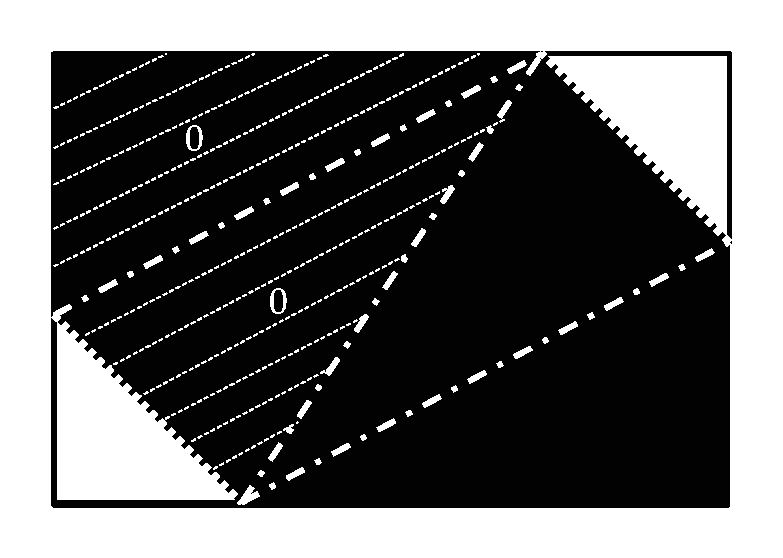
\includegraphics[width=\linewidth]{subphase_algorithm_2.eps}
		} &
		\subfloat[Move on to the next cell in the list that shares the same main phase value, and continue checking the connectivity.]{
			\label{fig:subphase_algorithm_3}
			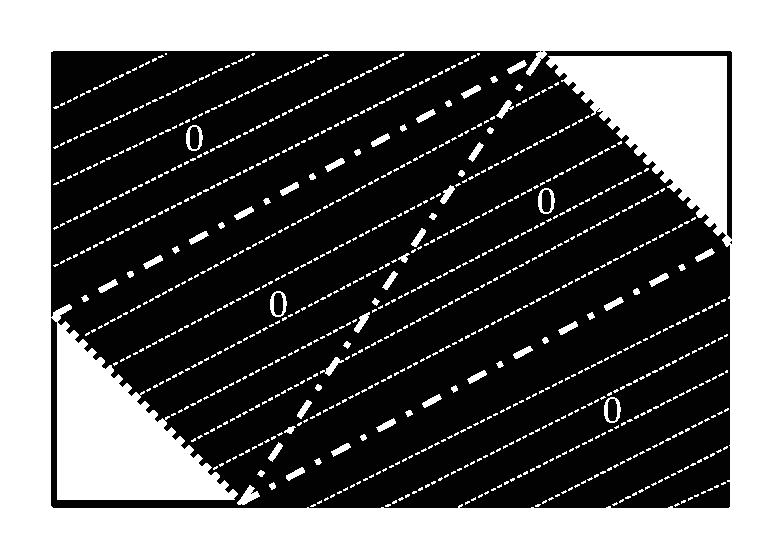
\includegraphics[width=\linewidth]{subphase_algorithm_3.eps}
		} \\
		\subfloat[Once the connectivity for the specific subphase of the main phase is achieved, check if additional cells have the same main phase but different subphase. If there are not any cells with the same main phase, move on the next main phase.]{
			\label{fig:subphase_algorithm_4}
			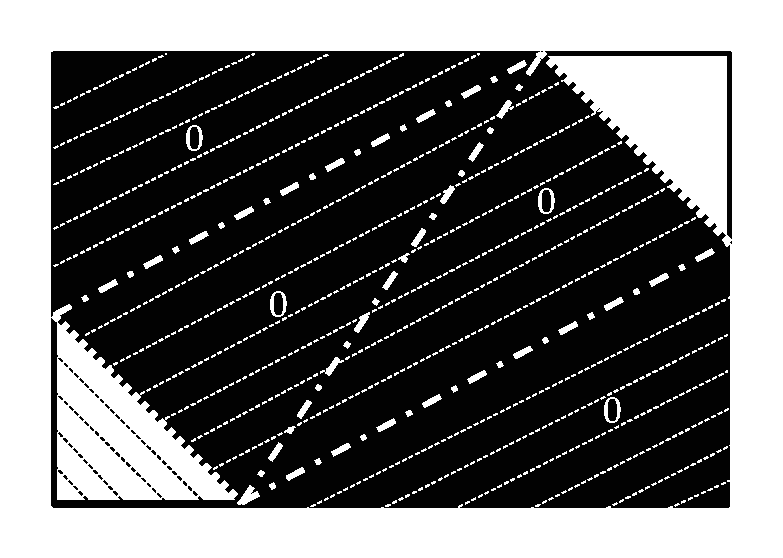
\includegraphics[width=\linewidth]{subphase_algorithm_4.eps}
		} &
		\subfloat[Select the first subphase of the second main phase. Repeat steps 1 through 3.]{
			\label{fig:subphase_algorithm_5}
			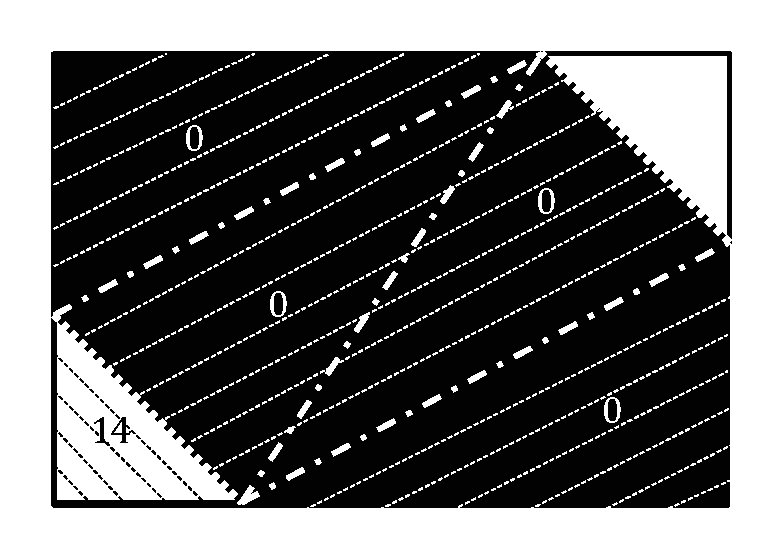
\includegraphics[width=\linewidth]{subphase_algorithm_5.eps}
		} &
		\subfloat[Once the connectivity for a subphase is computed, increase the subphase value within the main phase. Look for cells in the triangulation list that have not been processed yet, and check their connectivity.]{
			\label{fig:subphase_algorithm_6}
			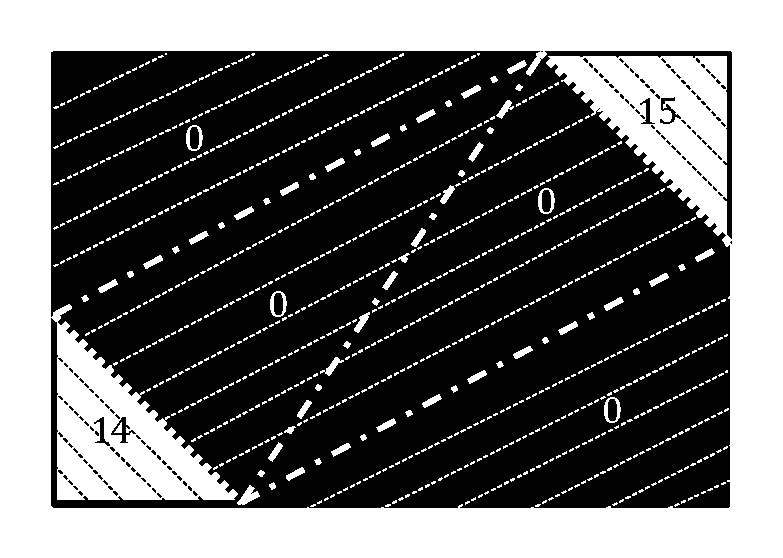
\includegraphics[width=\linewidth]{subphase_algorithm_6.eps}
		}
	\end{tabularx}
	\caption[Subphase computation algorithm.]{Subphase computation algorithm. Refer to section \ref{sec:main-phase-sub-phase} for a more detailed description.}
	\label{fig:subphase_algorithm}
\end{figure}

For Figure \ref{fig:subphase_algorithm}, we would get the list in table \ref{tab:main-phase-sub-phase-table}:

\begin{table}[htbp]
	\centering
		\begin{tabular}{| l | l | l |}
		\hline
		Triangle number & Main Phase & Sub-Phase \\ \hline
		1 & 1 & 0 \\ \hline
		2 & 1 & 0 \\ \hline
		3 & 1 & 0 \\ \hline
		4 & 1 & 0 \\ \hline
		5 & 2 & 1 \\ \hline
		6 & 2 & 2 \\ \hline
		\end{tabular}
	\caption[Main-phase and sub-phase table for pseudo-elements]{Main-phase and sub-phase table for pseudo-elements.}
	\label{tab:main-phase-sub-phase-table}
\end{table}

We have 6 different triangles generated by Delaunay triangulation. By convention, the order of the triangles is determined after the triangulation so that all phase 1 ones are located at the top, followed by the phase 2 triangles. Each triangle is assigned a main phase and sub-phase (see Table \ref{tab:main-phase-sub-phase-table}); the assignment is stored, using a one-to-one map by the XFEM element.

% -----------------------------------------------------------------------------

\subsubsection{Nodal enrichments for pseudo-elements}

To interpolate fields in the XFEM elements we need to determine which nodal enrichments are used within each pseudo element.  The enrichments need to be chosen such that the interpolations are continuous across adjacent elements within the same main phase and unique within pseudo elements of the main sub-phase but topologically disconnected.

The main concept of the procedure is to clearly separate element-level and node-level operations. This separation enables the parallelization of the procedure. The first step is to determine the enrichment levels a particular node will use to interpolate fields in the triangulated elements with a particular sub-phase. This step is done by looping over all nodes. The result of this loop is a map that links the sub-phase information of an element to an enrichment level for each node of the element. In a second step we loop over all elements to update the enrichment levels of pseudo-element based on the map built previously.

Looping over all nodal clusters, we build the following node-element table. The entries in the table are the sub-phases at the nodes within each element. The consistency node numbers are marked by a ``C''. Consistency nodes can be identified by nodes which have entries in more than one column; so they can be identified easily on the fly.

Two conditions, consistency and uniqueness, must be satisfied to ensure the assigned sub-phases are consistent across the nodal cluster. The consistency condition is satisfied if all sub-phases in a row are the same. The uniqueness condition is satisfied if the sub-phase of each set of connected nodes is unique in the cluster.

\begin{table}[htbp]
	\centering
		\begin{tabular}{| l | p{2cm} | p{2cm} | p{2cm} | p{2cm} |}
		\hline
		Nodes/Elements & 1 & 2 & 3 & 4 \\ \hline
		1 		& 14	&		&		&		 \\ \hline
		2 ``C''	&  0	&  0	&		&		 \\ \hline
		3 ``C''	& 15	& 14	& 14	& 15	 \\ \hline
		4 ``C''	&  0	&		&		&  0 	 \\ \hline
		5		& 		& 15	&		& 		 \\ \hline
		6 ``C''	&  		&  0	&  0	&		 \\ \hline
		7		&		& 		& 15	&		 \\ \hline
		8 ``C''	&		&  		&  0	&  0	 \\ \hline
		9		&		&		&		& 14	 \\ \hline
		\end{tabular}
	\caption[Initial node-element table]{Initial node-element table.}
	\label{tab:initial-node-element-table}
\end{table}

The initial node-element table (see Table \ref{tab:initial-node-element-table}) shows that the consistency condition is not satisfied since node 3 is inconsistent. Also, nodes 5 and 7, for example, should be assigned a unique sub-phase. Therefore the uniqueness condition is also not satisfied. To ensure both conditions we build a second table and where we iteratively correct the sub-phase until all conditions are satisfied. Note that the consistency and uniqueness checks are not needed for a 1 element cluster. The correction procedure is as follows:

\begin{enumerate}
\item Initialize a list of all sub-phase possible; mark them as unused; initialize a list of checked nodes. Mark all nodes as unchecked; build list of consistency nodes.
\item Ensure consistency: Repeat the following steps until all consistency nodes are checked.
	\begin{itemize}
	\item Select node: Start with the center node, which must be a consistency node (remember that this consistency and uniqueness check will not be applied for a one-element cluster). Otherwise select the first unchecked consistency node.
	\item Select sub-phase: Select the lowest unused sub-phase. Mark the selected sub-phase as used (keep consistency of sub-phase to the respective main phase).
	\item Identify connected consistency nodes and connected unique nodes:
		\begin{itemize}
		\item For each element to which the selected node belongs, connected nodes have the same sub-phase as the selected node has for this particular element. Select the connected nodes which may be either consistency or unique nodes. 
		\item In order to identify all connected consistency and unique nodes, search the connected elements for additional connected consistency and unique nodes.
		\item The above process requires recursively (a) searching for nodes within an element with the same sub-phase and (b) identifying elements that share consistency nodes. Note: the sub-phase id might change between elements if the sub-phases are not consistent yet for a consistency node.
		\end{itemize}
	\item Assign sub-phase: Assign the selected sub-phase to all connected nodes identified in the search process described above. For any value that needs to be changed, flip sub-phases for that element. Mark connected nodes as checked.
	\end{itemize}

\begin{table}[htbp]
	\centering
		\begin{tabular}{| l | p{2cm} | p{2cm} | p{2cm} | p{2cm} |}
		\hline
		Nodes/Elements & 1 & 2 & 3 & 4 \\ \hline
		1 		& 14 $\to$ 15	&		&		&		 		\\ \hline
		2 ``C''	&  0			&  0	&		&		 		\\ \hline
		3 ``C''	& 15 $\to$ 14	& 14	& 14	& 15$\to$ 14 	\\ \hline
		4 ``C''	&  0			&		&		&  0 	 		\\ \hline
		5		& 				& 15	&		& 		 		\\ \hline
		6 ``C''	&  				&  0	&  0	&		 		\\ \hline
		7		&				& 		& 15	&		 		\\ \hline
		8 ``C''	&				&  		&  0	&  0	 		\\ \hline
		9		&				&		&		& 14$\to$ 15	\\ \hline
		\end{tabular}
	\caption[Flipping the enrichment levels]{Flipping the enrichment levels to keep consistency.}
	\label{tab:flipping-enrichment-levels-table}
\end{table}

\item Ensure uniqueness: Loop through the remaining unchecked nodes. For each element, collect the unique nodes with an unused sub-phase, assign the next unused sub-phase to these nodes and check the sub-phase as being used. Here nodes 1, 5, 7, and 9 are assigned the sub-phase 16, 17, and 18, respectively (node 1 was flipped initially, but it was not marked as checked). The outcome of the above correction procedure is Table \ref{tab:final-node-element-table}:

\begin{table}[htbp]
	\centering
		\begin{tabular}{| l | p{2cm} | p{2cm} | p{2cm} | p{2cm} |}
		\hline
		Nodes/Elements & 1 & 2 & 3 & 4 \\ \hline
		1 		& 15		&		&		&		 \\ \hline
		2 ``C''	&  0		&  0	&		&		 \\ \hline
		3 ``C''	& 14		& 14	& 14	& 14	 \\ \hline
		4 ``C''	&  0		&		&		&  0 	 \\ \hline
		5		& 			& 16	&		& 		 \\ \hline
		6 ``C''	&  			&  0	&  0	&		 \\ \hline
		7		&			& 		& 17	&		 \\ \hline
		8 ``C''	&			&  		&  0	&  0	 \\ \hline
		9		&			&		&		& 18	 \\ \hline
		\end{tabular}
	\caption[Final node-element table]{The result of the enrichment algorithm. Nodes that are shared across elements receive the same enrichment level.}
	\label{tab:final-node-element-table}
\end{table}

\item Using the original and the corrected node-element tables we can build the map for the central point (here node ID 3). See Table \ref{tab:element-to-enrichment-table}. The rows correspond to the elements, the columns list the original sub-phases, and the entries are the enrichment levels used by the central node. When building this table we check that the map is consistent within itself (the same sub-phases within each are assigned to the same enrichments).

\begin{table}[htbp]
	\centering
		\begin{tabular}{| l | p{2cm} | p{2cm} | p{2cm} | p{2cm} |}
		\hline
		For Node 3:		& 0	& 14	& 15\\
		Element / Enrichment level & & &\\ \hline
		1 & 0 & 15 & 14 \\ \hline
		2 & 0 & 14 & 16 \\ \hline
		3 & 0 & 14 & 17 \\ \hline
		4 & 0 & 18 & 14 \\ \hline
		\end{tabular}
	\caption[Element to enrichment table]{Element to enrichment table for node ID 3. This table shows the initial enrichments node 3 received during the sub-phase algorithm and the enrichment levels after the enrichment algorithm.}
	\label{tab:element-to-enrichment-table}
\end{table}

\item With this map we can loop over all elements and assign enrichment levels for each node to each pseudo-element, based on their sub-phase information.
\end{enumerate}

% -----------------------------------------------------------------------------

\subsubsection{Determine degrees-of-freedom used}

The last step in the algorithm is to flag which enrichment levels each node will use for interpolation. For example, in our test case, node 3 will have enrichment levels 0, 14, 15, 16, 17, 18 active.

% -----------------------------------------------------------------------------

\subsubsection{Implementation example 2}

\begin{figure}[H]
	\centering
	\begin{tabularx}{0.75\linewidth}{X}
		\subfloat[Discrete model.]{
			\label{fig:physical_model_2}
			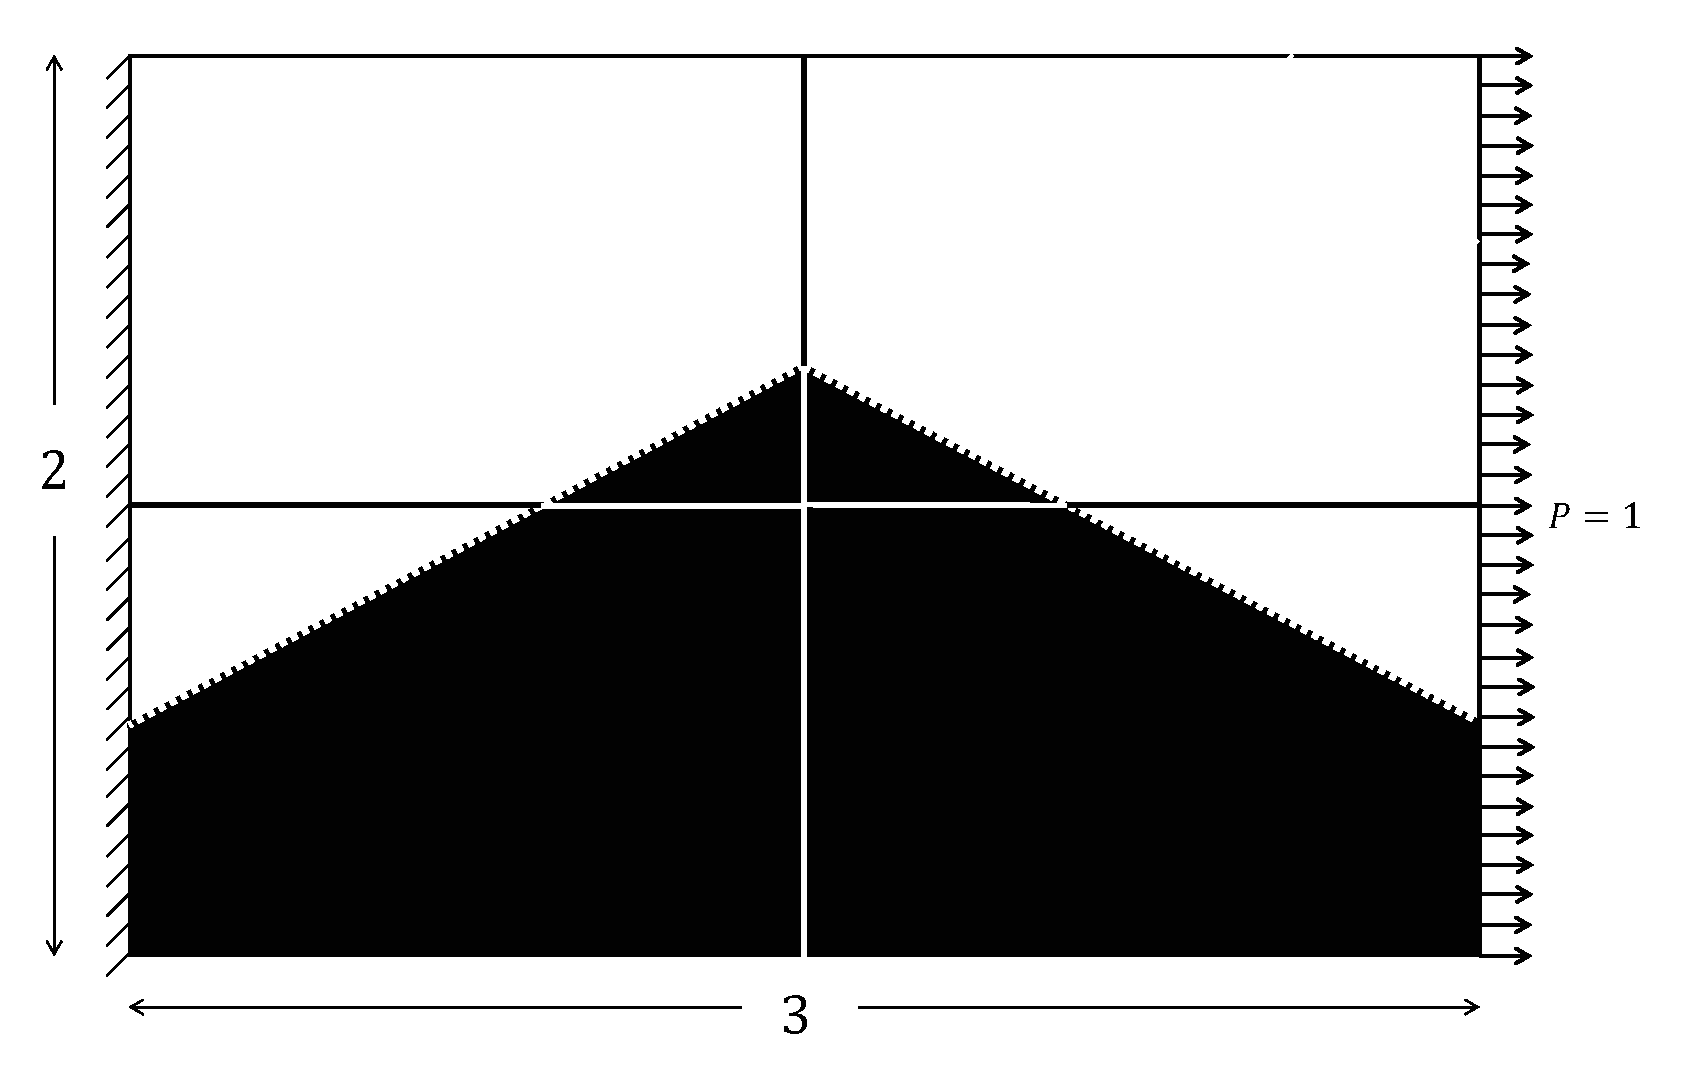
\includegraphics[width=\linewidth]{physical_model_2.eps}
		} \\
		\subfloat[Mesh information.]{
			\label{fig:discrete_model_2}
			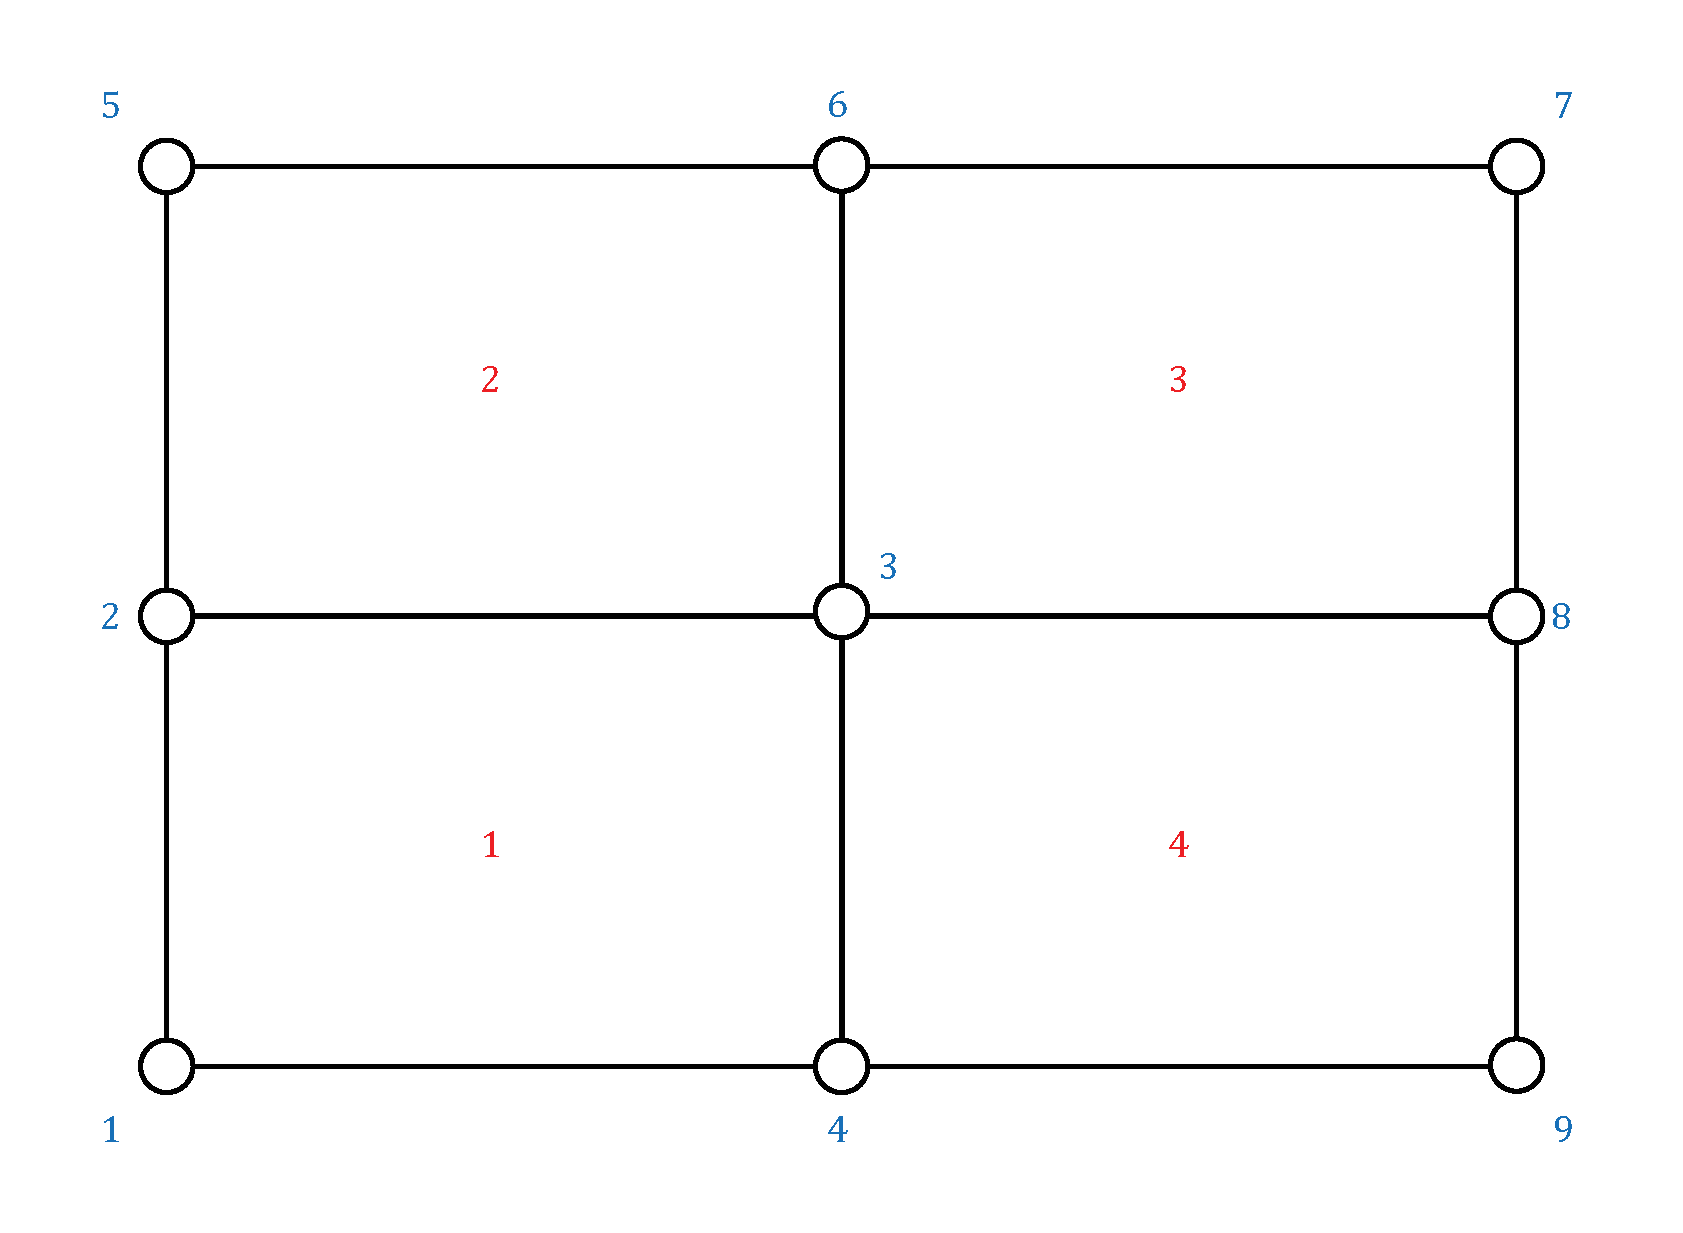
\includegraphics[width=\linewidth]{discrete_model.eps}
		}
	\end{tabularx}
	\caption[XFEM implementation example 2.]{XFEM implementation configuration 2.}
	\label{fig:implementation_example_2}
\end{figure}

\begin{table}[H]
	\centering
		\begin{tabular}{| l | p{2cm} | p{2cm} | p{2cm} | p{2cm} |}
		\hline
		Nodes/Elements & 1 & 2 & 3 & 4 \\ \hline
		1 		&  0		&		&		&		 \\ \hline
		2 ``C''	& 14		& 14	&		&		 \\ \hline
		3 ``C''	&  0		&  0	&  0	&  0	 \\ \hline
		4 ``C''	&  0		&		&		&  0 	 \\ \hline
		5		& 			& 14	&		& 		 \\ \hline
		6 ``C''	&  			& 14	& 14	&		 \\ \hline
		7		&			& 		& 14	&		 \\ \hline
		8 ``C''	&			&  		& 14	& 14	 \\ \hline
		9		&			&		&		&  0	 \\ \hline
		\end{tabular}
	\caption[Initial node-element table configuration 2]{Initial node-element table for configuration 2.}
	\label{tab:initial-node-element-table-configuration-2}
\end{table}

\begin{table}[H]
	\centering
		\begin{tabular}{| l | p{2cm} | p{2cm} | p{2cm} | p{2cm} |}
		\hline
		Nodes/Elements & 1 & 2 & 3 & 4 \\ \hline
		1 		&  0		&		&		&		 \\ \hline
		2 ``C''	& 14		& 14	&		&		 \\ \hline
		3 ``C''	&  0		&  0	&  0	&  0	 \\ \hline
		4 ``C''	&  0		&		&		&  0 	 \\ \hline
		5		& 			& 14	&		& 		 \\ \hline
		6 ``C''	&  			& 14	& 14	&		 \\ \hline
		7		&			& 		& 14	&		 \\ \hline
		8 ``C''	&			&  		& 14	& 14	 \\ \hline
		9		&			&		&		&  0	 \\ \hline
		\end{tabular}
	\caption[Final node-element table configuration 2]{Final node-element table for configuration 2.}
	\label{tab:final-node-element-table-configuration-2}
\end{table}

\begin{table}[H]
	\centering
		\begin{tabular}{| l | p{2cm} | p{2cm} | p{2cm} |}
		\hline
		For Node 3:		& 0	& 14 \\
		Element / Enrichment level & & \\ \hline
		1 & 0 & 14 \\ \hline
		2 & 0 & 14 \\ \hline
		3 & 0 & 14 \\ \hline
		4 & 0 & 14 \\ \hline
		\end{tabular}
	\caption[Element to enrichment table configuration 2]{Enrichment level map for configuration 2.}
	\label{tab:element-to-enrichment-table-2}
\end{table}

% -----------------------------------------------------------------------------

\subsubsection{Implementation example 3}

\begin{figure}[H]
	\centering
	\begin{tabularx}{0.75\linewidth}{X}
		\subfloat[Discrete model.]{
			\label{fig:physical_model_3}
			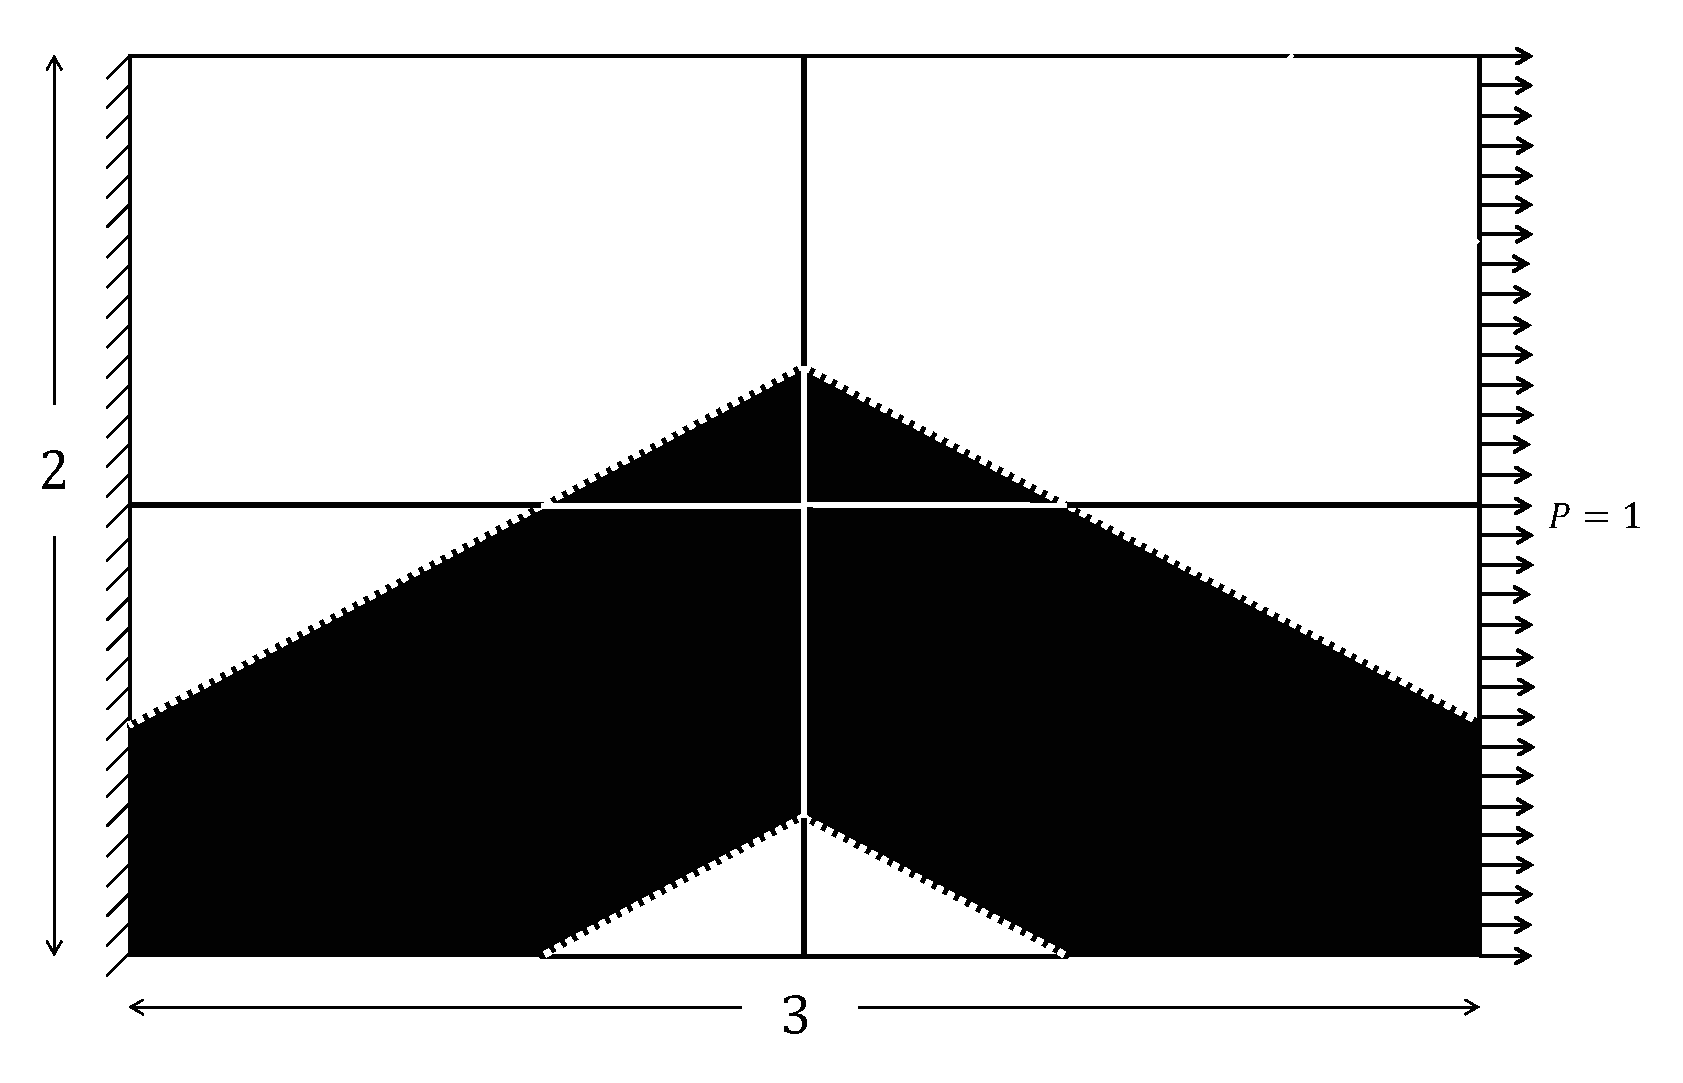
\includegraphics[width=\linewidth]{physical_model_3.eps}
		} \\
		\subfloat[Mesh information.]{
			\label{fig:discrete_model_3}
			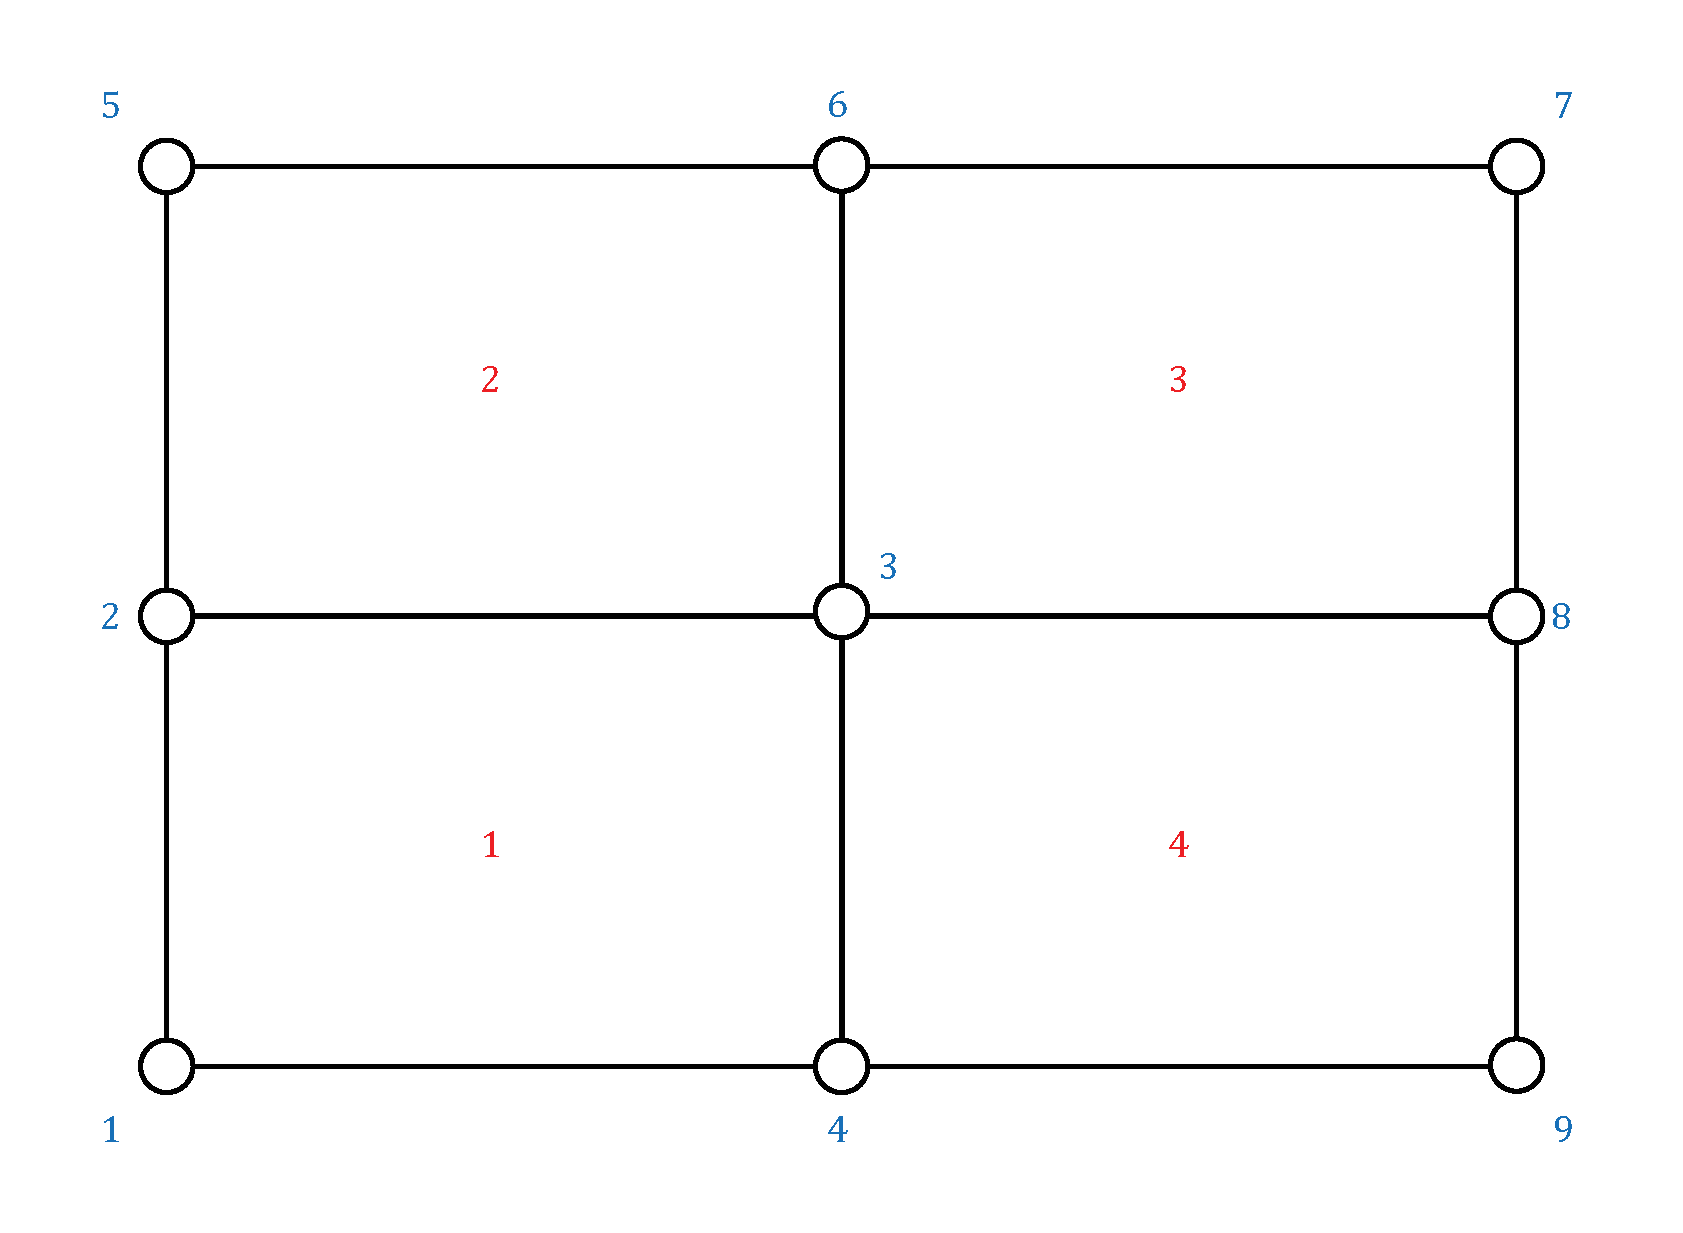
\includegraphics[width=\linewidth]{discrete_model.eps}
		}
	\end{tabularx}
	\caption[XFEM implementation example 3.]{XFEM implementation configuration 3.}
	\label{fig:implementation_example_3}
\end{figure}

\begin{table}[H]
	\centering
		\begin{tabular}{| l | p{2cm} | p{2cm} | p{2cm} | p{2cm} |}
		\hline
		Nodes/Elements & 1 & 2 & 3 & 4 \\ \hline
		1 		&  0		&		&		&		 \\ \hline
		2 ``C''	& 15		& 14	&		&		 \\ \hline
		3 ``C''	&  0		&  0	&  0	&  0	 \\ \hline
		4 ``C''	& 14		&		&		&  0 	 \\ \hline
		5		& 			& 14	&		& 		 \\ \hline
		6 ``C''	&  			& 14	& 14	&		 \\ \hline
		7		&			& 		& 14	&		 \\ \hline
		8 ``C''	&			&  		& 14	& 15	 \\ \hline
		9		&			&		&		&  0	 \\ \hline
		\end{tabular}
	\caption[Initial node-element table configuration 3]{Initial node-element table for configuration 3.}
	\label{tab:initial-node-element-table-configuration-3}
\end{table}

\begin{table}[H]
	\centering
		\begin{tabular}{| l | p{2cm} | p{2cm} | p{2cm} | p{2cm} |}
		\hline
		Nodes/Elements & 1 & 2 & 3 & 4 \\ \hline
		1 		&  0		&		&		&		 \\ \hline
		2 ``C''	& 14		& 14	&		&		 \\ \hline
		3 ``C''	&  0		&  0	&  0	&  0	 \\ \hline
		4 ``C''	& 15		&		&		& 15	 \\ \hline
		5		& 			& 14	&		& 		 \\ \hline
		6 ``C''	&  			& 14	& 14	&		 \\ \hline
		7		&			& 		& 14	&		 \\ \hline
		8 ``C''	&			&  		& 14	& 14	 \\ \hline
		9		&			&		&		&  0	 \\ \hline
		\end{tabular}
	\caption[Final node-element table for configuration 3]{Final node-element table for configuration 3.}
	\label{tab:final-node-element-table-configuration-3}
\end{table}

\begin{table}[H]
	\centering
		\begin{tabular}{| l | p{2cm} | p{2cm} | p{2cm} |}
		\hline
		For Node 3:		& 0	& 14 & 15\\
		Element / Enrichment level & & & \\ \hline
		1 & 0 & 15 & 14	\\ \hline
		2 & 0 & 14 &   	\\ \hline
		3 & 0 & 14 &   	\\ \hline
		4 & 0 & 15 & 14	\\ \hline
		\end{tabular}
	\caption[Element to enrichment table configuration 3]{Enrichment level map for configuration 3.}
	\label{tab:element-to-enrichment-table-3}
\end{table}

% -----------------------------------------------------------------------------

\subsection{Solving the problem}

In the previous section, our algorithms determined which additional enriched degrees-of-freedom each node requires to account for the discontinuities in the elements. We will study our enrichment strategy with a heat conduction problem. To capture the discontinuities along the phase boundaries, we enrich the standard finite element approximation with additional shape functions. We adopt the generalized enrichment strategy of \citet{MM:13} which resolves consistently the temperature fields in the presence of small features and does not suffer from artificially coupling disconnected phases.
%
\begin{equation}
	u(\mathbf{x}) = \sum \limits^{M}_{m=1} \left( H(-\phi) \sum\limits^{n}_{i=1} \mathbf{N}_i \ u_{i,m}^A
														 + H( \phi) \sum\limits^{n}_{i=1} \mathbf{N}_i \ u_{i,m}^B \right)
\end{equation}

where $m$ is the enrichment level, $M$ is the maximum number of enrichment levels used for each phase, $\mathbf{N}$ are the shape functions, $u^l_{i,m}$ is the vector of nodal temperature values at node $i$ for phase $l=[A,B]$, $\phi$ is the level set value evaluated at the integration point, and $H$ denotes the Heaviside function.

The Heaviside function $H$ depends on the level set function and is defined as follows:
%
\begin{equation}
	H(z) =
		\begin{cases}
			1 & z > 0 \\
			0 & z \le 0
		\end{cases}
\end{equation}

The Heaviside functions ``turns on/off'' the standard finite element interpolations in the particular phases. The approximation allows for discontinuities of the temperatures along the phase boundaries. Therefore the continuity is enforced weakly via the stabilized Lagrange multiplier method.

% -----------------------------------------------------------------------------

\subsection{Preconditioner}

When a sub-domain of a material phase is too small (around $O(\epsilon^{1/2})$), the Jacobian matrix will be ill-conditioned. To solve this shortcoming, it is necessary to scale the matrix with another preconditioning matrix. This scaling matrix will be a function of the level-set field.

The preconditioner $\pmb{T}$ will have a scaling value for each degree of freedom in the problem. To obtain these values, we check which enriched degrees of freedom each node uses. Then, we proceed to compute the integral of the shape function for the node with respect to the material sub-domain that requires said enriched degree-of-freedom. Because a node will have different scaling values across multiple elements, there are four preconditioner implementations available to compute the scaling value in a nodal cluster:

\begin{itemize}
\item Maximum value of integrals of shape functions
\item Sum of values of integrals of shape functions
\item Maximum value of integrals of the derivatives of the shape functions
\item Sum of values of integrals of the derivatives of the shape functions
\end{itemize}

The third preconditioner approach will be used in this study. The matrix $\pmb{T}$ is a diagonal matrix built by integrating the spatial derivatives of the shape functions over the nodal support of nodes connected to an intersected element. The diagonal components of the matrix are defined as:
%
\begin{equation}
	\pmb{T}_{i,m}^{l} = \left( \max_{e \in E_{i}} \frac { \int_{\mathcal{D}_l^e} \nabla \mathbf{N}_i(\mathbf{x}) \cdot
	\nabla
	\mathbf{N}_i(\mathbf{x}) \,d\mathbf{x}}{\int_{\mathcal{D}^e} \nabla \mathbf{N}_i(\mathbf{x}) \cdot \nabla
	\mathbf{N}_i(\mathbf{x}) \,d\mathbf{x}} \right)^{-1/2}
\end{equation}
%
where $\pmb{T}_{i,m}^{l}$ corresponds to the degree-of-freedom $\mathbf{u}_{i,m}^{l}$, $i$ is the node index, $l=[A,B]$ is the material phase, $m$ is the enrichment level, $E_{i}$ is the set of elements connected to node $i$, and $\mathcal{D}_l^e$ is the element domain of phase $l$. The components of the matrix increase as the region of influence of a degree-of-freedom decreases. The entries $\pmb{T}_{i,m}^{l}$ of nodes $i$ that are not connected to at least one intersected element are set to one.

To avoid numerical issues due to large values for the components of $\pmb{T}$, the degrees of freedom associated with the diagonal entry $\pmb{T}_{i,m}^{l}$ are constrained to zero if the following condition is satisfied:
%
\begin{equation}
	\pmb{T}_{i,m}^{l} \ge T_{tol}
\end{equation}
%
where $T_{tol}$ is $10^9$ for this study.

At this point, there is one scaling value for each degree-of-freedom in the system. These scaling values are applied to the solution vector before the computation of the residual. After the residual is computed, they are both unscaled and then the new solution vector is computed. 
\section{Corroboration and results}
\label{corroboration_results}

% -----------------------------------------------------------------------------
% Methodology

\subsection{Methodology}

Two formulations were used to corroborate the results of the XFEM implementation.

Equation \ref{eq:interface-error} computes the difference in solutions at the discontinuity. Since the model we have implemented is based on inclusions and not crack propagation, this interface error should approach zero as the mesh gets finer.
%
\begin{equation}
	\sqrt{\frac{\sum_{\mathrm{element}} \sum_{\mathrm{interface}} \int u^+-u^- \mathrm{d}\Gamma_i}{\sum_{\mathrm{element}} \sum_{\mathrm{interface}} \int \mathrm{d}\Gamma_i}}
	\label{eq:interface-error}
\end{equation}

This equation computes the interface ``jump'' across all interfaces and elements in the model, then scales it with respect to the perimeter or area of the interface, and finally takes the square root.

Equation \ref{eq:L2-error} compares the relative difference between the XFEM solution and the FEM solution.
%
\begin{equation}
	\sqrt{\frac{\int u_{\mathrm{XFEM}}-u_{\mathrm{FEM}} \mathrm{d}\Omega}{\int u_{\mathrm{FEM}} \mathrm{d}\Omega}}
	\label{eq:L2-error}
\end{equation}

$u_{\mathrm{XFEM}}$ represents the XFEM solution, while $u_{\mathrm{FEM}}$ represents the FEM solution.

XFEM was used to solve a thermal problem with the configuration of Figure \ref{fig:thermal-setup}. The same problem was ran using the classical FEM. The FEM problem used two different types of elements and its mesh was refined until the solution reached convergence.
%
\begin{figure}[htbp]
	\centering
	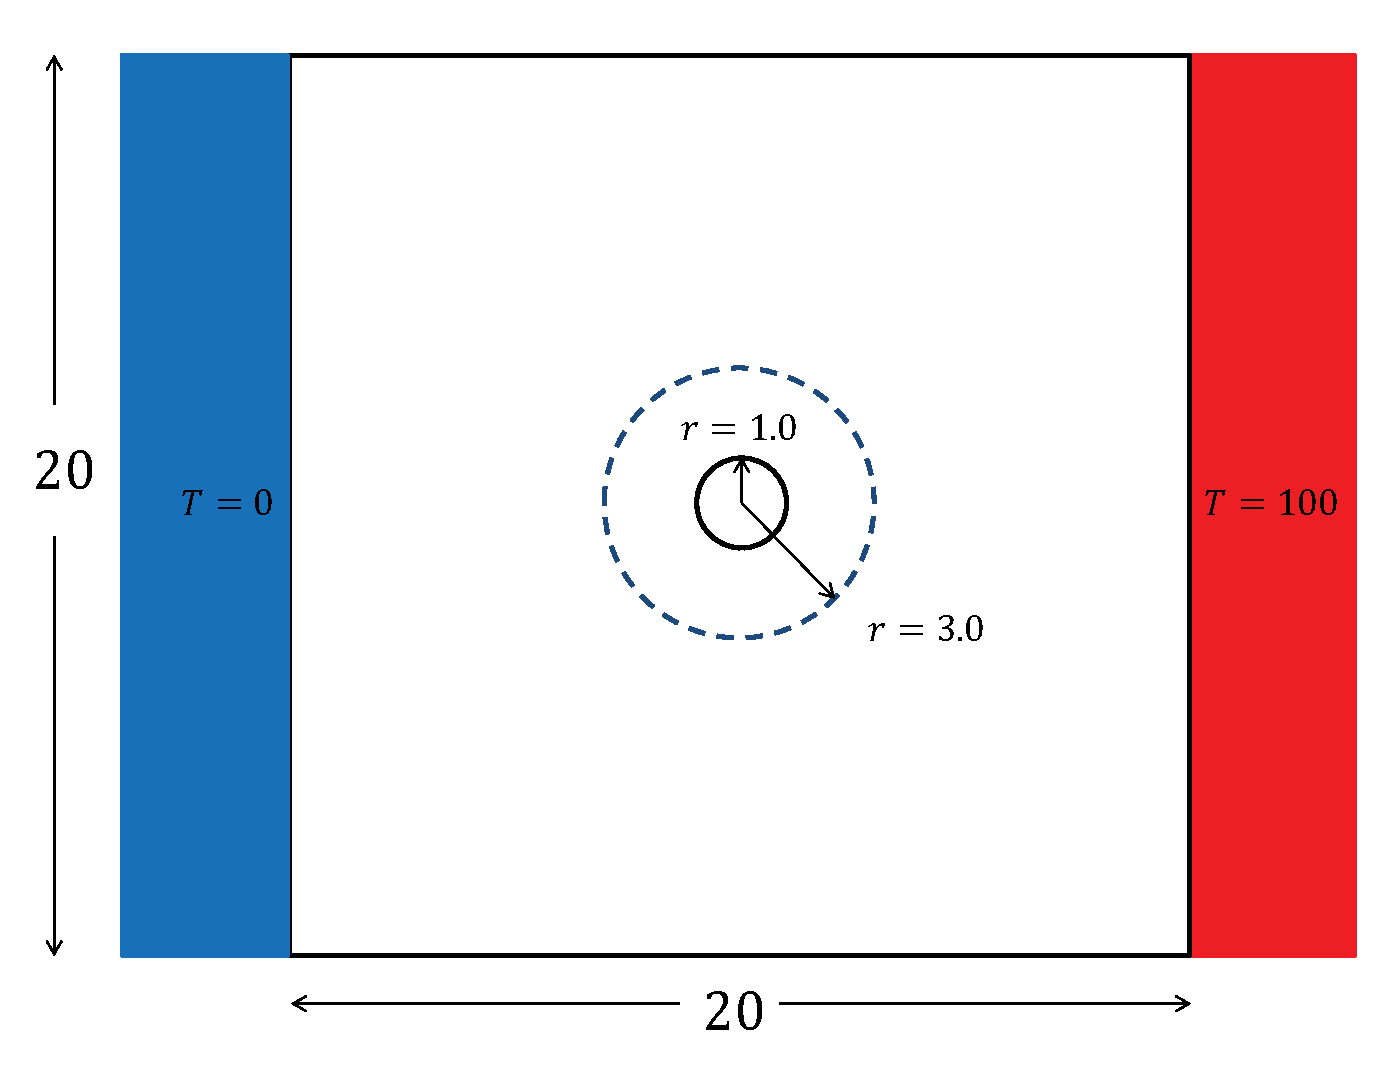
\includegraphics[width=0.75\linewidth]{diffusion_setup.eps}
	\caption[Diffusion problem setup]{Diffusion problem setup.}
	\label{fig:thermal-setup}
\end{figure}

The mesh has a width of $20$ units and a height of $20$ units. The problem has Dirichlet boundary conditions on the sides. The temperature is prescribed to $0$ on the left side and $100$ on the right side. There is an inclusion at the center of the model. This inclusion is a different material with a different thermal conductivity than the material phase $1$ domain.

The test consisted in modifying the diameter of the circle from $2$ units to $6$ units in $500$ steps using different mesh refinements, different conductivity ratios and different preconditioners formulations.

% -----------------------------------------------------------------------------
% Tests

\subsection{Tests}

% -----------------------------------------------------------------------------
% Mesh refinement

\subsubsection{Mesh refinement sweep}

The mesh size was the variable in this test, while the conductivity ratio between both materials remained fixed at 10. No preconditioner scaling was applied. The different mesh sizes used were $20 \times 20$, $30 \times 30$, $40 \times 40$, and $50 \times 50$.

Figure \ref{fig:mesh-sweep-interface} shows that as the mesh is refined, the interface error converges to zero.

\begin{figure}[H]
	\centering
	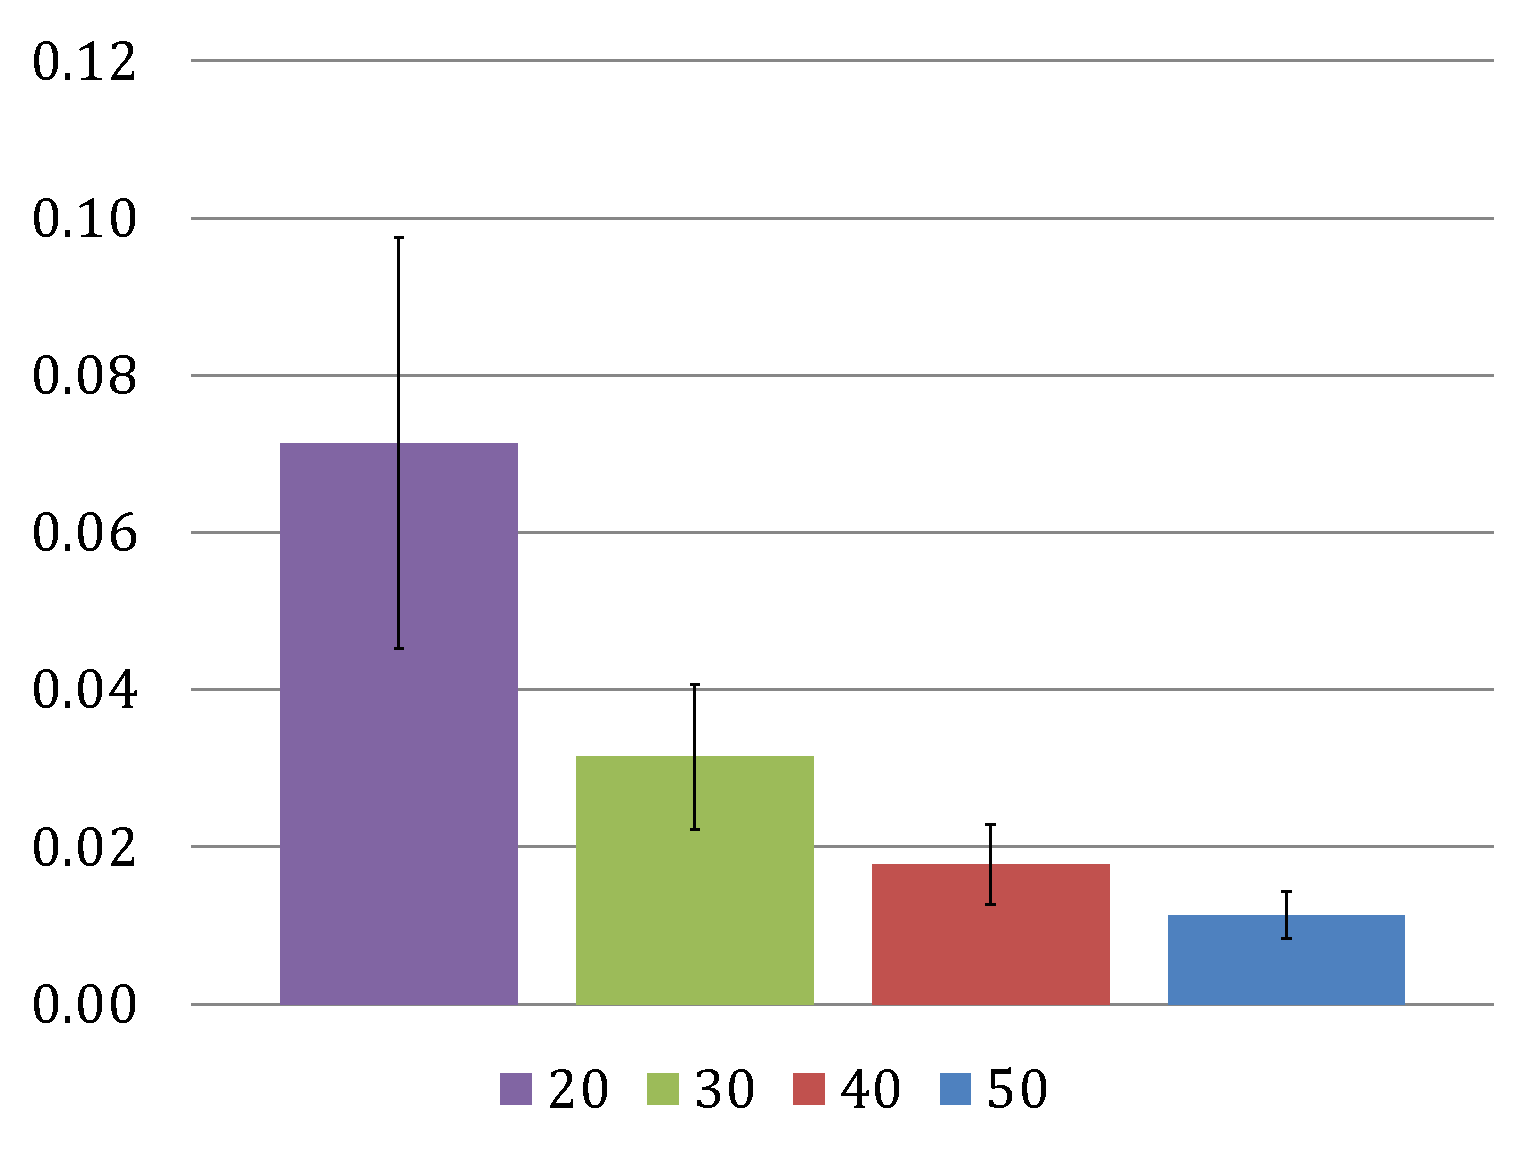
\includegraphics[width=0.5\linewidth]{mesh_sweep_interface.eps}
	\caption[Mesh refinement sweep interface error]{Mesh refinement sweep interface error.}
	\label{fig:mesh-sweep-interface}
\end{figure}

Figure \ref{fig:mesh-sweep-L2} shows that as the mesh is refined, the difference of the XFEM solution with respect to the FEM solution decreases. The larger difference for the $50 \times 50$ mesh is due to the sampling and different mesh sizes used for the XFEM and FEM problems. A different mesh resampling size fixed the issue in other tests.
%
\begin{figure}[H]
	\centering
	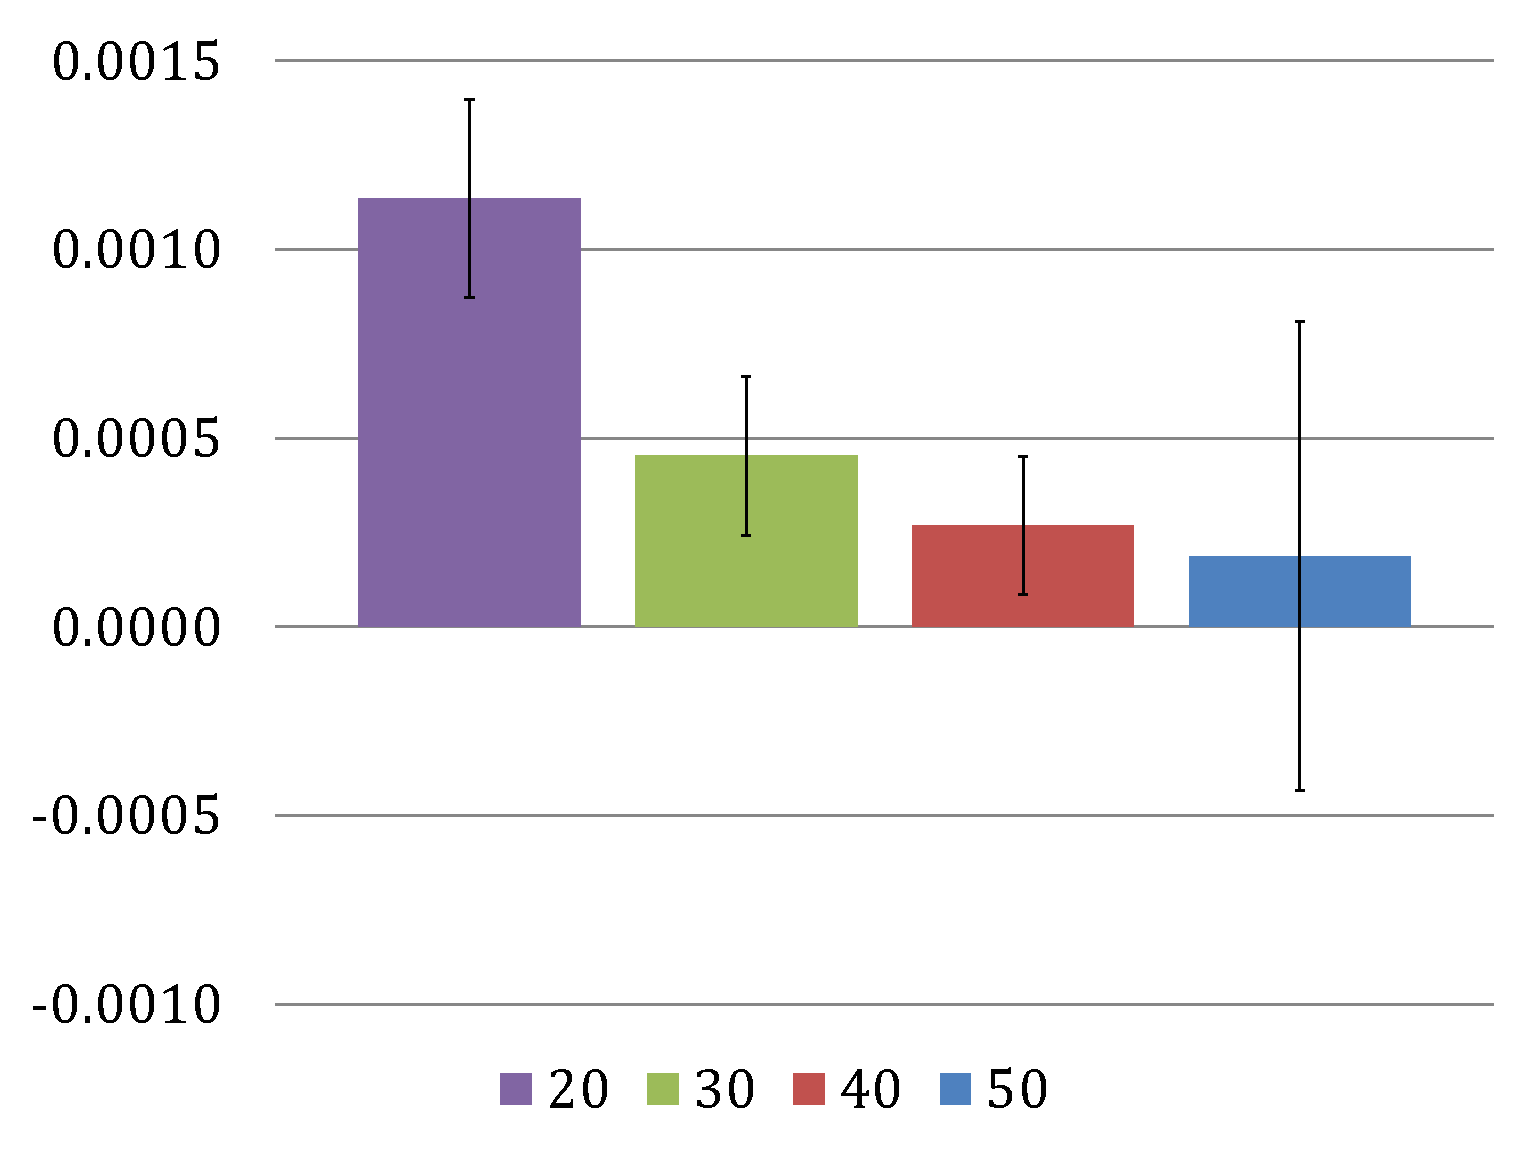
\includegraphics[width=0.5\linewidth]{mesh_sweep_L2.eps}
	\caption[Mesh refinement sweep L2 error]{Mesh refinement sweep L2 error.}
	\label{fig:mesh-sweep-L2}
\end{figure}
%
% -----------------------------------------------------------------------------

\subsubsection{Conductivity ratio sweep}

The conductivity ratio between the different materials was the variable in this test. The mesh size was $30 \times 30$ and the preconditioner formulation used the maximum spatial derivative of the shape functions. The different conductivity ratios used were 0.1, 10, 100, and 1000.

Figure \ref{fig:conductivity-sweep-interface} shows that when the material conductivity is the same for both materials (a ``quasi-FEM'' problem), the interface error is in the order of $O(\epsilon)$. However, the greater the difference in material properties at an interface, the larger the interface jump is.
%
\begin{figure}[H]
	\centering
	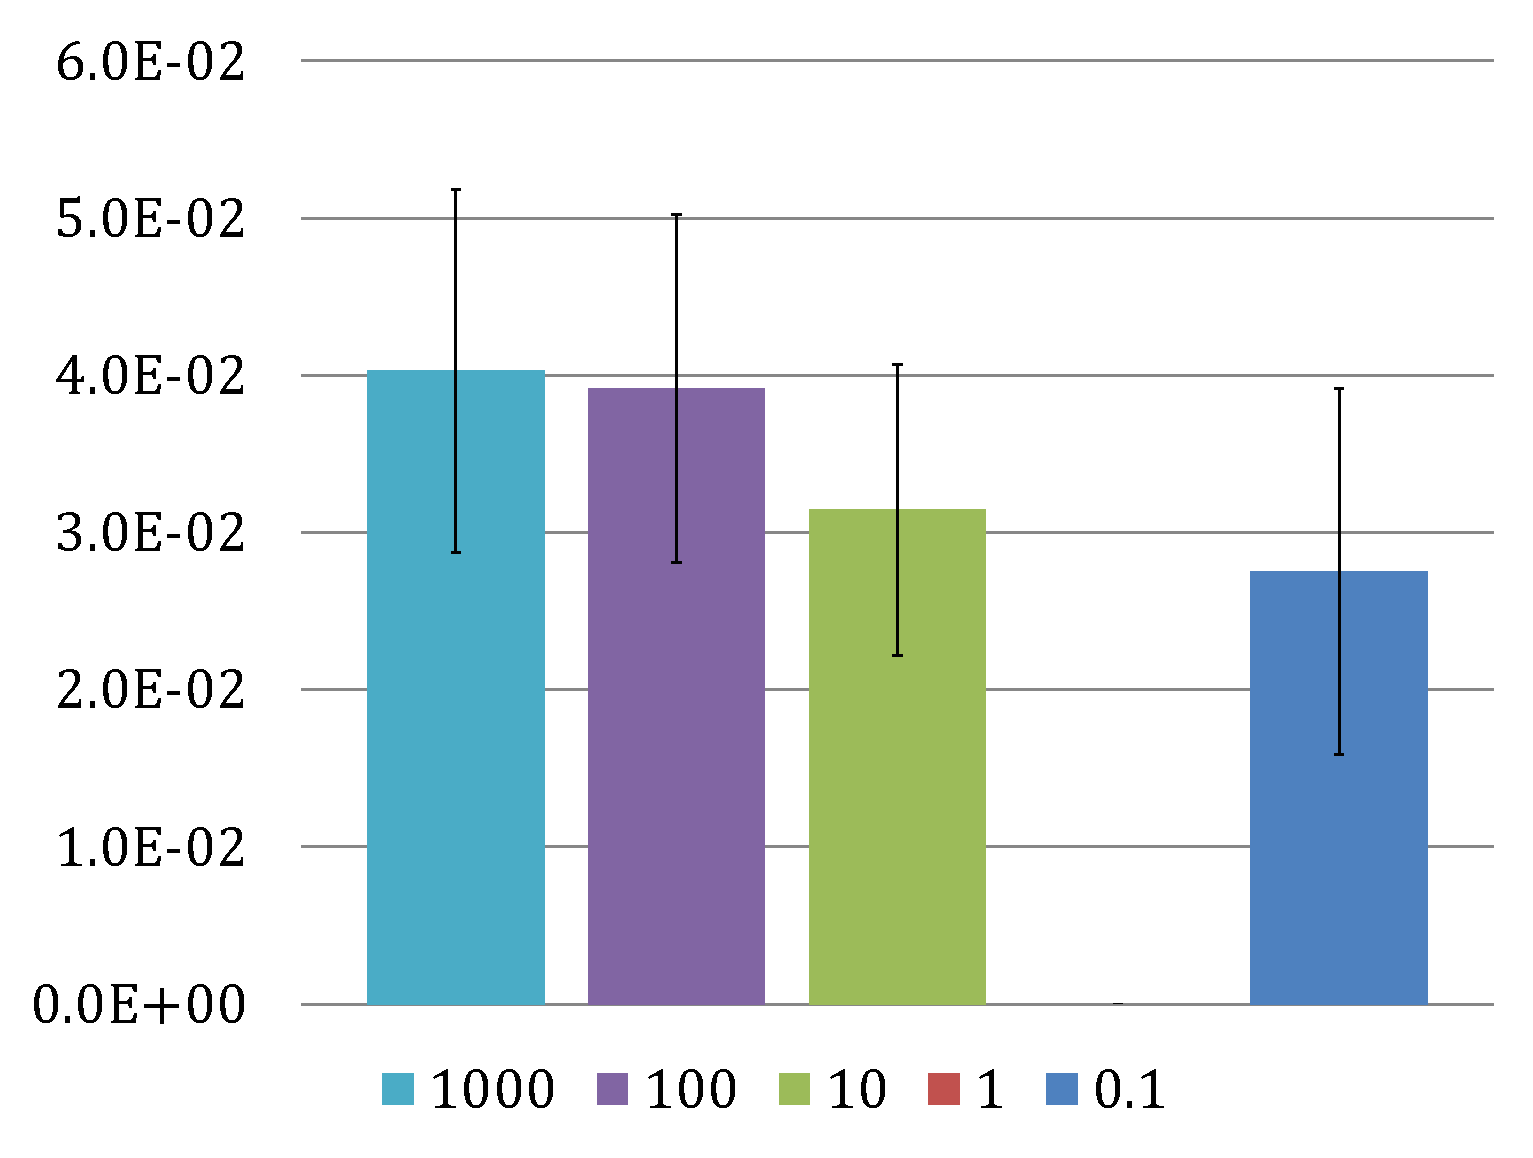
\includegraphics[width=0.5\linewidth]{conductivity_sweep_interface.eps}
	\caption[Conductivity refinement sweep interface error]{Conductivity refinement sweep interface error.}
	\label{fig:conductivity-sweep-interface}
\end{figure}

For the L2 computation, only FEM solutions with conductivity ratios of 10, 100, and 1000 were computed. Figure \ref{fig:conductivity-sweep-L2} shows that the difference in solutions is very small ~$O(10^{-4})$.
%
\begin{figure}[H]
	\centering
	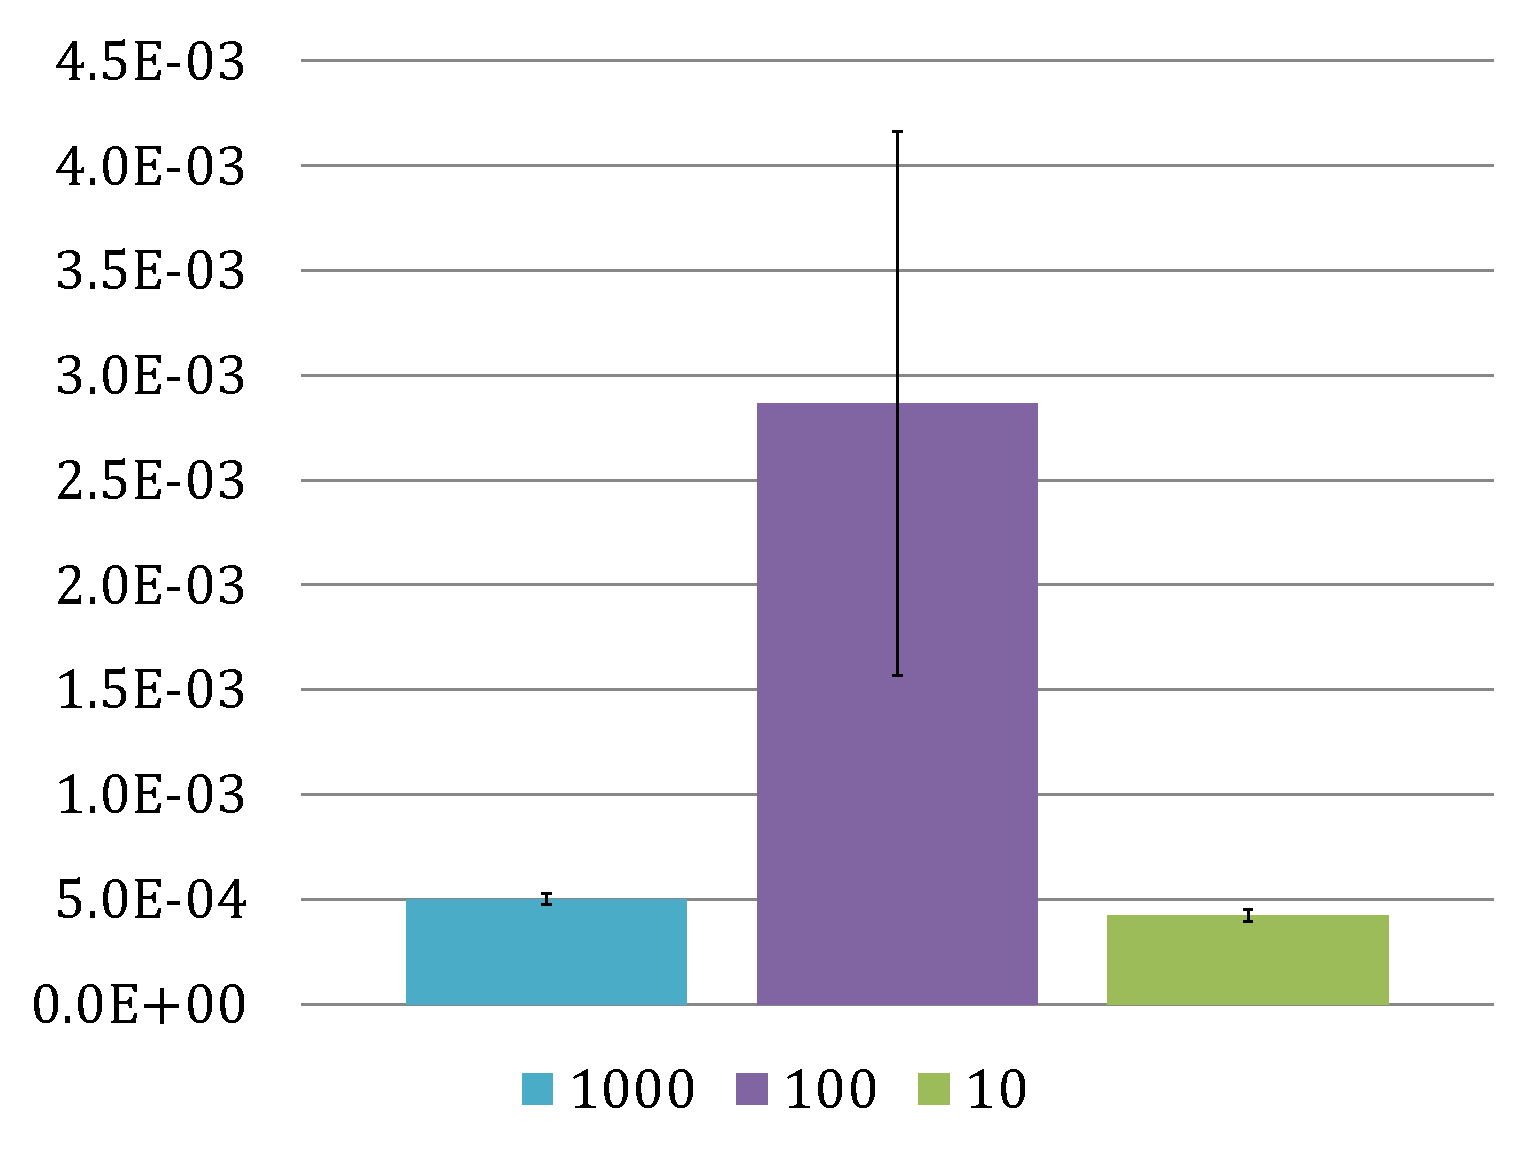
\includegraphics[width=0.5\linewidth]{conductivity_sweep_L2.eps}
	\caption[Conductivity refinement sweep L2 error]{Conductivity refinement sweep L2 error.}
	\label{fig:conductivity-sweep-L2}
\end{figure}
%
% -----------------------------------------------------------------------------

\subsubsection{Condition number comparison}

These tests were performed to compare the condition number of the global Jacobian matrix when the scaling was applied. The mesh size was $30 \times 30$, the conductivity ratio was 10 and the preconditioner formulation used the maximum spatial derivative of the shape functions. A direct solver and a GMRES iterative solver were used and compared.

Figure \ref{fig:condition_number_no_scaling} shows that the Jacobian matrix has a condition number in the order of $10^{15}$ when no scaling is applied \footnote{We use the GMRES solver provided by the Trilinos linear algebra package to solve for the linear system. The solver uses an ILU preconditioner on top of the XFEM preconditioner of this study. However, the condition number of the matrix, after the ILU preconditioner is applied, is not provided by the Trilinos package. Because of that, the direct and iterative solver yield the same condition number. In reality, the GMRES option may have a lower condition number due to the ILU preconditioner.}, while Figure \ref{fig:condition_number_scaling} shows that the condition number decreases to the order of $10^4$ when scaling is applied.
%
\begin{figure}[htbp]
	\centering
	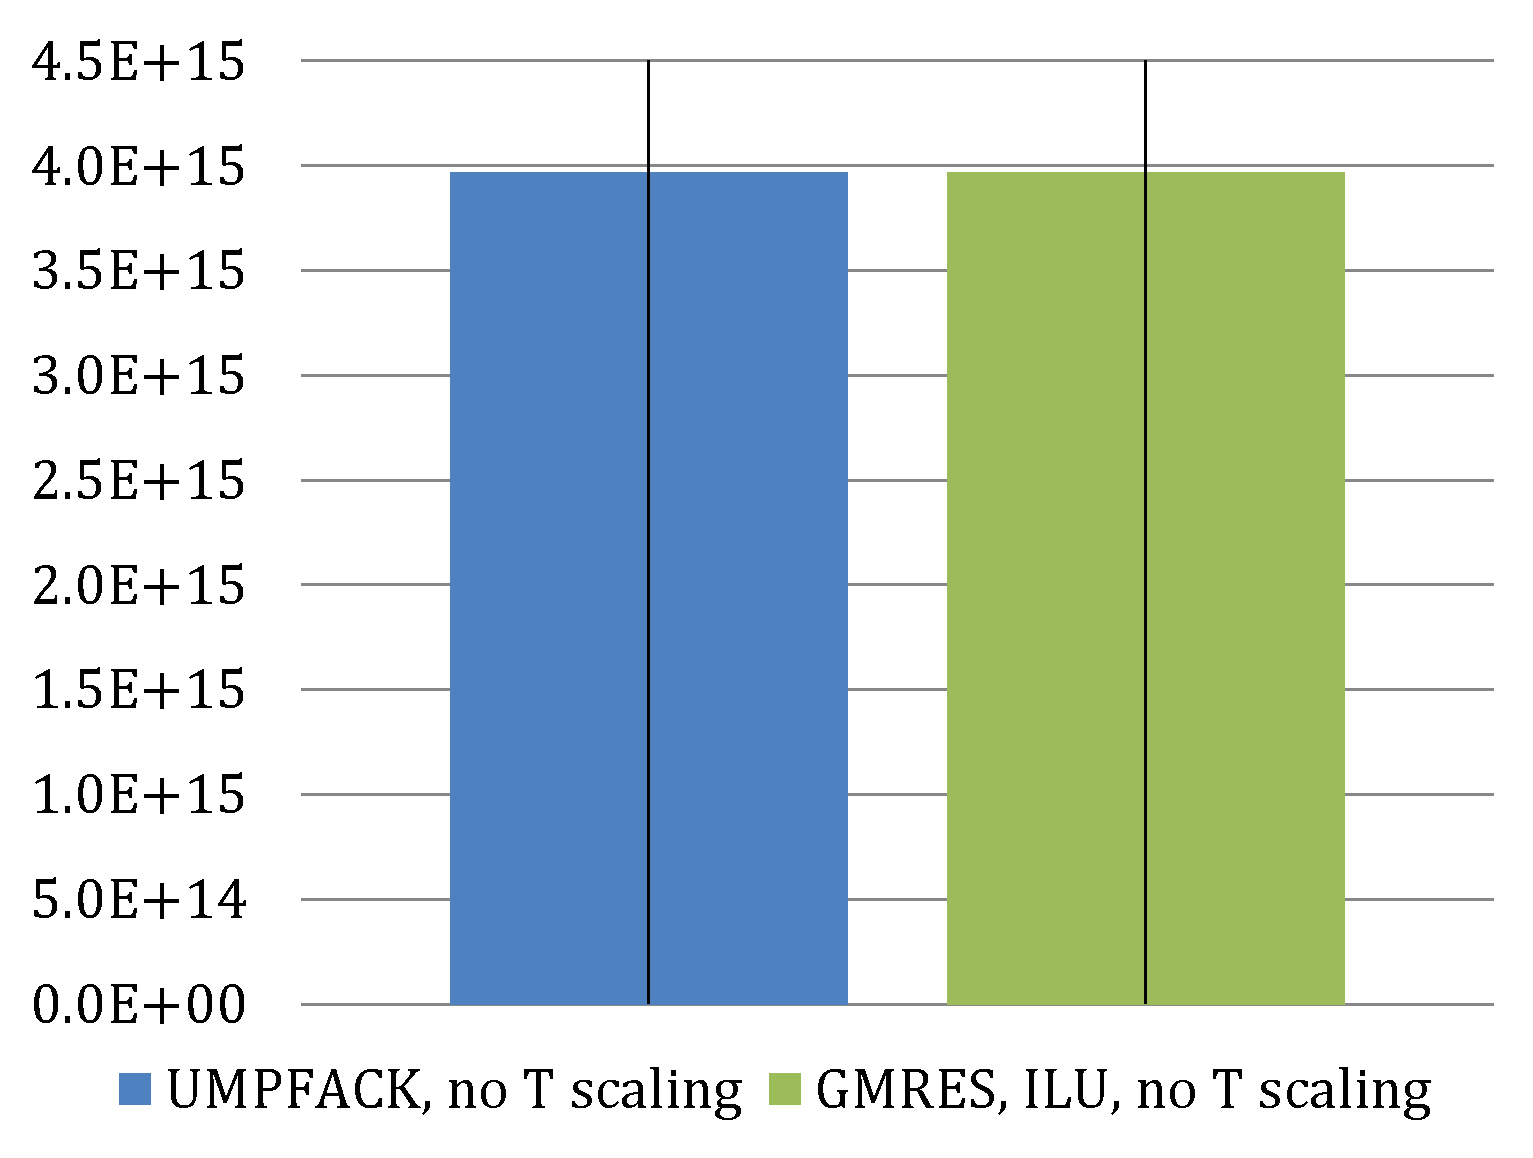
\includegraphics[width=0.5\linewidth]{condition_number_no_scaling.eps}
	\caption[Condition number comparison - no preconditioner]{Condition number comparison - no pre-conditioner.}
	\label{fig:condition_number_no_scaling}
\end{figure}
%
\begin{figure}[htbp]
	\centering
	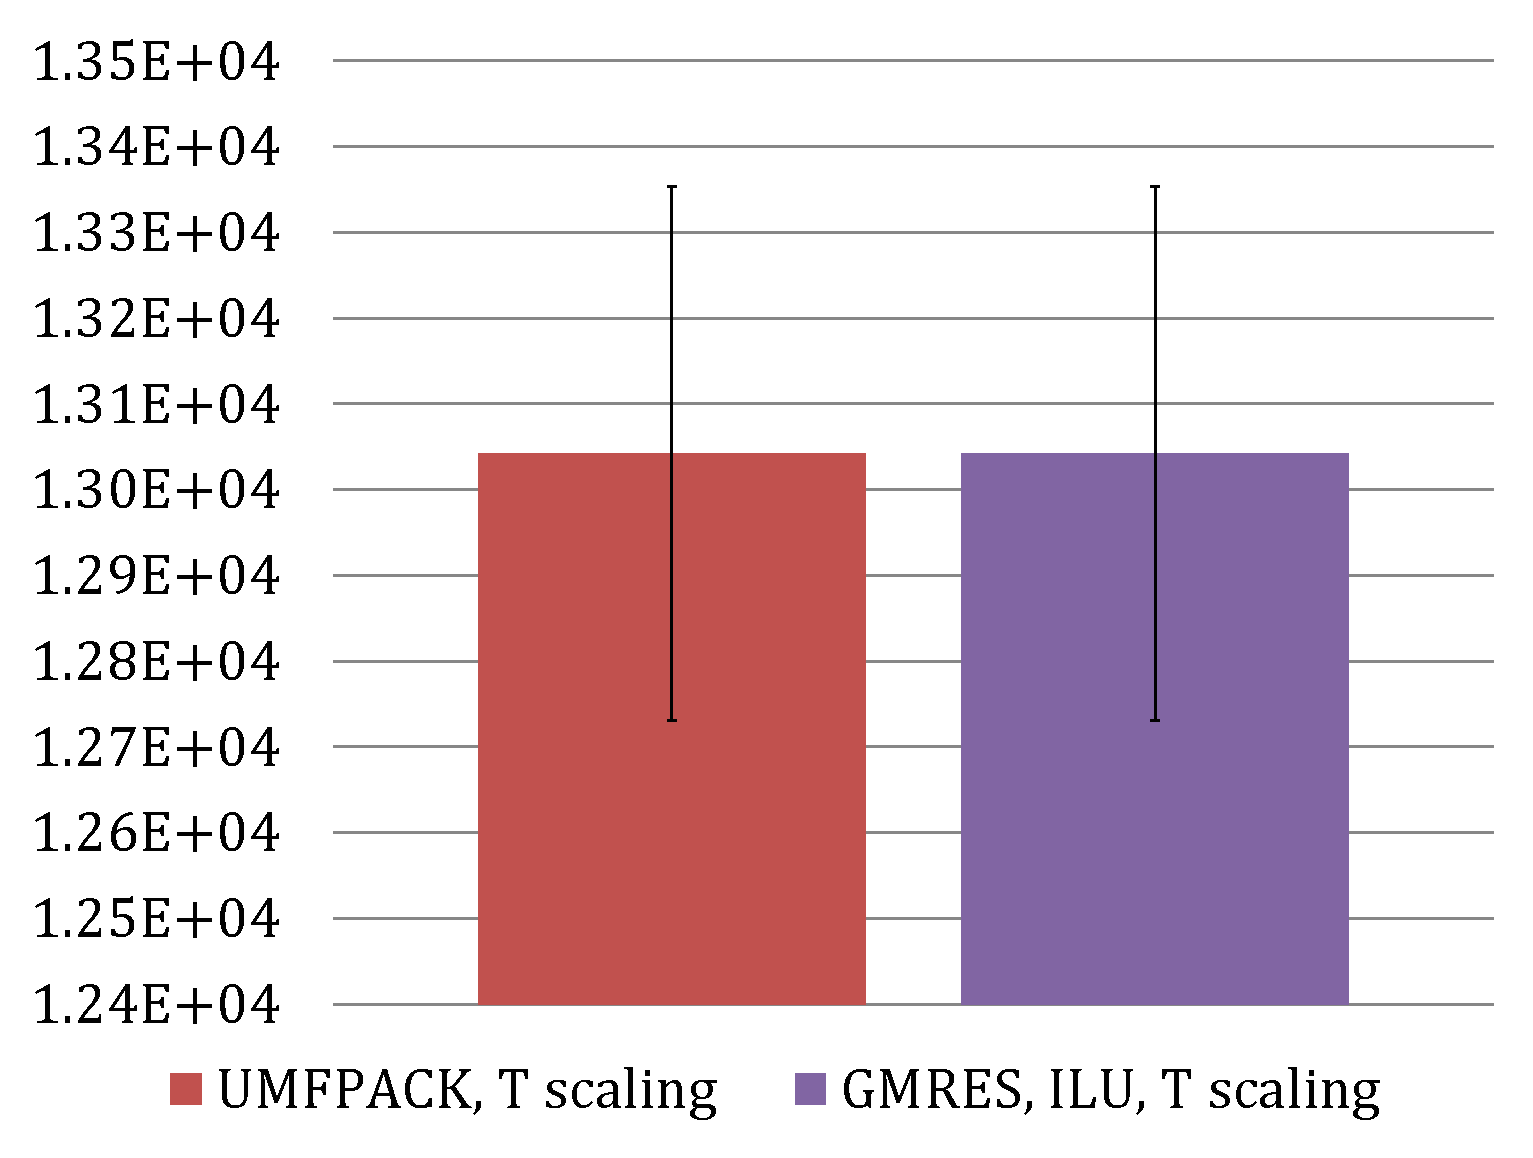
\includegraphics[width=0.5\linewidth]{condition_number_scaling.eps}
	\caption[Condition number comparison - with preconditioner]{Condition number comparison - with pre-conditioner.}
	\label{fig:condition_number_scaling}
\end{figure} 
%\section{Conclusions and Future Work}
\section{Conclusions}
\label{sec:implementation_conclusions}

% -----------------------------------------------------------------------------

%\subsection{Conclusions}

The framework developed in this project will help eliminate the need to re-mesh a model when discontinuities present in the domain. The program is capable of dividing an element into integrable sub-domains, calculating its topology, its enrichment information and computing the normal vector and Gauss points required for integration. The program is also capable of solving XFEM problems with different topologies in 3D.

Results showed that the differences in solutions with a classical FEM problem for a two dimensional heat conduction model are small.

XFEM produced Jacobian matrices with high condition numbers, but the application of a preconditioner as a function of the level set field solved this shortcoming.

%\subsection{Future work}
%
%Future work in this project involves the implementation of the algorithms in a parallel environment. The framework for a parallel algorithm would include two intermediate steps: one between the sub-phase computation and the enrichment level computation and another after the enrichment level algorithm and before the solution of the problem. The first exchange would communicate sub-phase information from elements connected to a node across separate processors. The second exchange of information would send and receive the different enriched degrees of freedom across elements on multiple processors. This last exchange would follow the rules of classical parallel FEM code for coupled problems where two elements have different degrees of freedom. 

% -----------------------------------------------------------------------------
% Appendices

\section{Appendix A: Delaunay Triangulation code}
\label{sec:delaunay_triangulation_code}

This code written in Matlab is the first attempt of the author to perform a Delaunay triangulation in an element based on the level set function values at the corner nodes. To triangulate different discontinuities change the $levs$ variable: each entry corresponds to the value of the level set function at a node. The $e_x$, $e_y$, and $e_z$ vector variables contain the coordinates of the corner nodes and can be modified to change the shape of the element.

\lstset{language=Matlab,%
%	basicstyle=\color{red},
    breaklines=true,%
    morekeywords={matlab2tikz},
    keywordstyle=\color{blue},%
    morekeywords=[2]{1}, keywordstyle=[2]{\color{black}},
    identifierstyle=\color{black},%
    stringstyle=\color[RGB]{170,55,241},
    commentstyle=\color[RGB]{28,172,0},%
    showstringspaces=false,%without this there will be a symbol in the places where there is a space
    numbers=left,%
    numberstyle={\tiny \color{black}},% size of the numbers
    numbersep=9pt, % this defines how far the numbers are from the text
    emph=[1]{for,end,break},emphstyle=[1]\color{red}, %some words to emphasise
    basicstyle=\tiny,
%	emph=[2]{word1,word2}, emphstyle=[2]{style},    
}

% -----------------------------------------------------------------------------

\subsection{main.m}

\lstinputlisting{./src/a_complete_methodology_for_the_implementation_of_XFEM_inclusive_models/etc/matlab/main.m}

% -----------------------------------------------------------------------------

\subsection{xfem8isct.m}

\lstinputlisting{./src/a_complete_methodology_for_the_implementation_of_XFEM_inclusive_models/etc/matlab/xfem8isct.m}

% -----------------------------------------------------------------------------

\subsection{xfem8tet.m}

\lstinputlisting{./src/a_complete_methodology_for_the_implementation_of_XFEM_inclusive_models/etc/matlab/xfem8tet.m}

% -----------------------------------------------------------------------------

\subsection{number\_configurations.m}

\lstinputlisting{./src/a_complete_methodology_for_the_implementation_of_XFEM_inclusive_models/etc/matlab/number_configurations.m}